\documentclass[11pt,a4paper]{report}
\usepackage{polyglossia}
\usepackage{csquotes}
\setmainlanguage[variant=mono]{greek}
\setotherlanguage{english}
%\setmainfont[Mapping=tex-text]{CMU Serif} %Set Fonts	
\setmainfont[Mapping=tex-text]{Cambria} %Set Fonts
\usepackage{float} %Package needed in order to use \begin{figure}[H]
\usepackage{amsmath}
\usepackage{amsfonts}
\usepackage{amssymb}
\usepackage{makeidx} %Package needed in order to make indices
\usepackage{graphicx}
\usepackage{diagbox}
\graphicspath{{Εικόνες//}} % The path for pictures to be used
\usepackage[left=3.18cm,right=3.18cm,top=2.54cm,bottom=2.54cm,includefoot]{geometry}%we define texts geometry
\usepackage{siunitx} % Package for SI units like degrees
\usepackage{enumitem} % Package used to format the enumerated text 
\usepackage{subcaption}
\usepackage{color}
\usepackage{titlesec}
\usepackage{changepage}
\usepackage{lipsum} %Package needed to generate random text lorem ipsum.....
\usepackage[table,xcdraw]{xcolor}
\usepackage[nottoc]{tocbibind}
\setcounter{secnumdepth}{3}% numbering of subsubsections
\setcounter{tocdepth}{3}% include subsubsections
\usepackage{fancyhdr}
\fancyhf{}																					%**
\fancyhead[LE]{\textbf{\thepage}}  															%**
\fancyhead[RE]{ \nouppercase{\leftmark}}													%**
\fancyhead[RO]{\textbf{\thepage}}															%**
\fancyhead[LO]{ \nouppercase{\rightmark}}													%**
\fancyfoot[CE,CO]{}																			%**
\fancyfoot[LE,RO]{}	
\renewcommand{\footrulewidth}{0.4pt} %1pt = 0.0352777778 cm
%-------------------------------
\titleformat{\chapter}{}{}{0em}{\bf\LARGE} % to remove word Chapter N from the first page of each chapter
\pagenumbering{roman}
\usepackage{hyperref}% Package used to create hyperlinks. The last package of the preample
\hypersetup{pdfborder = 0 0 0}% This is used in order to eliminate the borders dimensions
\titleformat{\chapter}{}{}{0em}{\bf\LARGE} % to remove word Chapter N from the first page of each chapter
\setlength{\parindent}{0cm}% We set the indent of the paragraph
\setlength{\parskip}{1.0em}% We set the spacing of one paragraph to the other
\fontdimen2\font=4pt %define spacing between words
\graphicspath{{Figures//}{Pictures//}}
\begin{document}
\pagestyle{fancy}% This command makes footers and headers  
\thispagestyle{empty} % We remove page numbering

\begin{minipage}[c]{0.32\textwidth}
	\begin{minipage}[c]{0.48\textwidth}
		
\includegraphics[width=\textwidth]{ΠΑΠΕΙ.jpg}
	\end{minipage}
	\begin{minipage}[c]{0.48\textwidth}
			
\includegraphics[width=\textwidth]{ΔΗΜΟΚΡΙΤΟΣ.jpg}
	\end{minipage}
\end{minipage}
\begin{minipage}[c]{0.68\textwidth}
	\begin{Large}
		\textbf{Πανεπιστήμιο Πειραιώς} \\
		\textbf{ΕΚΕΦΕ “ΔΗΜΟΚΡΙΤΟΣ”} \\
	\end{Large}
	\begin{large}
		\textbf{Δ.Π.Μ.Σ. στην Τεχνητή Νοημοσύνη} \\
	\end{large}
	\begin{large}
		\textbf{Τμήμα Ψηφιακών Συστημάτων Πανεπιστημίου Πειραιώς} \\
	\end{large}
	\begin{large}
		\textbf{Ινστιτούτο Πληροφορικής και Τηλεπικοινωνιών ΕΚΕΦΕ «Δημόκριτος»} \\
	\end{large}
\end{minipage}
\begin{center}
	\begin{Large}
		\vspace{0.1\textheight}
		\textbf{Μεταφορά μάθησης σε Βαθιά Νευρωνικά Δίκτυα}\\
	\end{Large}	
	\vspace{0.15\textheight} 
	Εργασία στο μάθημα “Βαθιά Μηχανική Μάθηση”\\	
	\begin{Large}
		\vspace{0.05\textheight}
		\textbf{Νικόλαος Μακρής - mtn2208}\\
	\end{Large}
	\vspace{0.25\textheight} 
	Διδάσκων: Γιαννακόπουλος Θεόδωρος, Μεταδιδακτορικός Ερευνητής ΕΚΕΦΕ Δημόκριτος\\
	\vspace{\fill}
	Αθήνα, 20-7-2023
\end{center}
 
%---------------End of First Page--------------



\clearpage
\pagenumbering{roman}
%--------The table of contents--------------------------
\begingroup
\makeatletter \let\ps@plain\ps@empty \makeatother
\tableofcontents
\endgroup
%\mainmatter
%--------The chapters of this paper---------------------
\clearpage
\pagenumbering{arabic}
\chapter{Αρχικά Βήματα}
\thispagestyle{empty} % We remove page numbering
\vspace{-2em}
\section{Περιγραφή προβλήματος}
\label{Problem Description}
Σκοπός της συγκεκριμένης εργασίας ήταν η χρήση δύο διαφορετικών συνόλων δεδομένων (dataset) και η εκπαίδευση νευρωνικών δικτύων για κάθε ένα από αυτά. Επιπλέον το πρώτο μοντέλο θα έπρεπε να χρησιμοποιηθεί ως βάση για την εφαρμογή της μεθόδου της μεταφοράς μάθησης (transfer learning) κατά την εκπαίδευση του δεύτερου δικτύου. Η επιλογή των συνόλων δεδομένων και του τύπου του προβλήματος (π.χ. παλινδρόμηση, ταξινόμηση κλπ.) που χρησιμοποιήθηκαν ήταν ελεύθερη. 

Για τη συγκεκριμένη εργασία, επιλέχθηκε ένα πρόβλημα ταξινόμησης πολλών κλάσεων (multiclass classification), όπου με τη χρήση εικόνων γίνεται διάκριση μεταξύ διαφορετικών ειδών τροφής. Τα δύο datasets που χρησιμοποιήθηκαν είναι το UECFOOD256 \cite{kaggle_dataset_UECFOOD256} και το FOOD101 \cite{kaggle_dataset_FOOD101}.

Πιο συγκεκριμένα, το πρώτο dataset περιλαμβάνει περίπου 31000 φωτογραφίες 256 διαφορετικών τροφών με διαφορετικό αριθμό φωτογραφιών για κάθε μια από τις 256 κατηγορίες, με τις περισσότερες εξ αυτών να είναι κατηγορίες τροφών που συναντώνται στην Ιαπωνία. Στο δεύτερο σύνολο δεδομένων εντοπίζονται 101 κλάσεις με 1000 ακριβώς φωτογραφίες ανά κλάση. 

Τα δύο σύνολα έχουν κάποια κοινά στοιχεία, πχ υπάρχει η κλάση "πίτσα" και στα δύο, αλλά η μεγάλη πλειοψηφία των κλάσεων ανήκει αποκλειστικά σε ένα από τα δύο σύνολα. Η λογική που ακολουθήθηκε ήταν να επιλεγεί το πρώτο dataset και να εκπαιδευτεί πάνω σε αυτό ένας ταξινομητής (classifier) με όσο το δυνατόν μεγαλύτερη ακρίβεια πρόβλεψης του είδους της τροφής και εν συνεχεία να χρησιμοποιηθεί για μεταφορά μάθησης στο δεύτερο dataset. Στον πίνακα \ref{Food_datasets_table} παρατίθενται τα στοιχεία για το μέγεθος και τον αριθμό των κλάσεων των συνόλων δεδομένων που χρησιμοποιήθηκαν.

\begin{table}[H]
\centering
\begin{tabular}{|c|c|c|}
\hline
                & UECFOOD256 & FOOD101 \\ \hline
Κλάσεις         & 256        & 101     \\ \hline
Αριθμός εικόνων & 31651      & 101000  \\ \hline
\end{tabular}
\caption{Σύνολα δεδομένων (datasets)}
\label{Food_datasets_table}
\end{table}


\section{Περιγραφή παραδοτέου προγράμματος}
\label{Package Structure}

Πριν την αναλυτική περιγραφή των βημάτων που ακολουθήθηκαν για την εκπαίδευση των νευρωνικών δικτύων παρατίθεται μια σύντομη περιγραφή της δομής του παραδοτέου πακέτου κώδικα ώστε να υπάρχει μια εικόνα της σύνδεσης όλων όσων περιγράφονται στο υπόλοιπο κείμενο. Στο σχήμα \ref{Package_Structure_image} φαίνεται η δομή του παραδοτέου προγράμματος. Τα βασικά στοιχεία συνοψίζονται στα εξής.

\begin{enumerate}
\item dummy\_data: Φάκελος που περιέχει δεδομένα ΧΧΧΧΧΧΧ
\item logs :  Φάκελος ο οποίος δημιουργείται κατά τη διάρκεια της πρώτης εκτέλεσης του προγράμματος και περιέχει log αρχεία με χρήσιμες πληροφορίες για την πορεία εκτέλεσης του προγράμματος
\item myenv : Φάκελος που περιέχει το εικονικό περιβάλλον το οποίο χρησιμοποιήθηκε για την ανάπτυξη του κώδικα. Η ενεργοποίηση του γίνεται με βάση τις οδηγίες που υπάρχουν στο README αρχείο 
\item py\_imports :  Φάκελος που περιέχει τα διάφορα python scripts (κλάσεις, συναρτήσεις) που χρησιμοποιούνται στο κυρίως πρόγραμμα
\item py\_plots :  Φάκελος που περιέχει τις συναρτήσεις (κώδικας python) που χρησιμοποιούνται για τη δημιουργία διαφόρων σχημάτων και γραφικών παραστάσεων που χρησιμοποιούνται στην παρούσα αναφορά
\item results : Φάκελος αποτελεσμάτων που δημιουργείται κατά την πρώτη εκτέλεση του προγράμματος
\item main.py : Κυρίως πρόγραμμα python
\item .gitignore, README, environment : Αρχεία του git και του εικονικού περιβάλλοντος
\end{enumerate}


\begin{figure}[H]
\centering
\begin{subfigure}[t]{0.3\textwidth}%
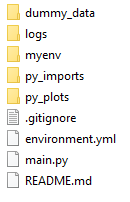
\includegraphics[width=\textwidth]{Program_Structure.png}
\end{subfigure}
\caption{Δομή προγράμματος}
\label{Package_Structure_image}
\end{figure}


\section{Προεπεξεργασία δεδομένων}
\label{Data pre-processing}

Οι εικόνες και των δύο dataset είναι διαφόρων διαστάσεων και αναλογιών πλάτους-ύψους, οπότε πριν την εκκίνηση της εκπαίδευσης παρεμβάλλεται υποχρεωτικά ένα βήμα προ-επεξεργασίας κατά το οποίο όλες οι εικόνες αποκτούν τις ίδιες διαστάσεις. Για τον σκοπό αυτό αναπτύχθηκε κώδικας ο οποίος αναλαμβάνει την μετατροπή των εικόνων στο επιθυμητό τελικό μέγεθος.

Επιπλέον, στο σύνολο δεδομένων UECFOOD256 δίνονται τα περιγράμματα (bounding boxes) που περικλείουν το είδος της τροφής προς ταξινόμηση και αποκλείουν όλο το περιβάλλον. Γίνεται λοιπόν χρήση μιας μεθόδου αποκοπής (cropping), ώστε να μείνει μόνο το συγκεκριμένο αντικείμενο εντός εικόνας και να διευκολυνθεί η διαδικασία της εκπαίδευσης επιτυγχάνοντας τελικά μεγαλύτερη ακρίβεια πρόβλεψης. Στην εικόνα \ref{Crop_image} φαίνεται το αποτέλεσμα της αποκοπής σε μια εικόνα του UECFOOD256. Σε όλες τις περιπτώσεις επιλέχθηκε η διατήρηση και των τριών καναλιών χρωμάτων σε κάθε εικόνα και η μη μετατροπή τους σε μονοχρωματικές για λόγους επίτευξης μεγαλύτερης ακρίβειας κατά τη διάρκεια της εκπαίδευσης, παρά το αυξημένο υπολογιστικό κόστος που αυτή η απόφαση συνεπάγεται.

\begin{figure}[H]
\centering
\begin{subfigure}[t]{0.5\textwidth}%
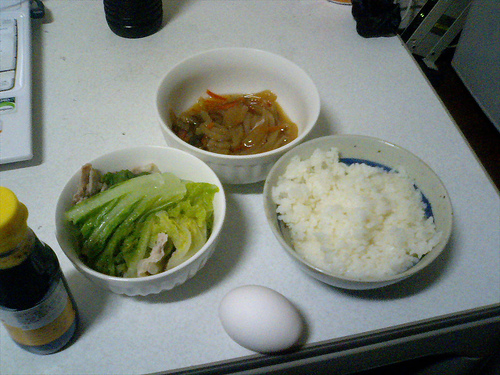
\includegraphics[width=\textwidth]{εικόνα_πριν.jpg}
\caption{Πριν}
\end{subfigure}%
\begin{subfigure}[t]{0.5\textwidth}%
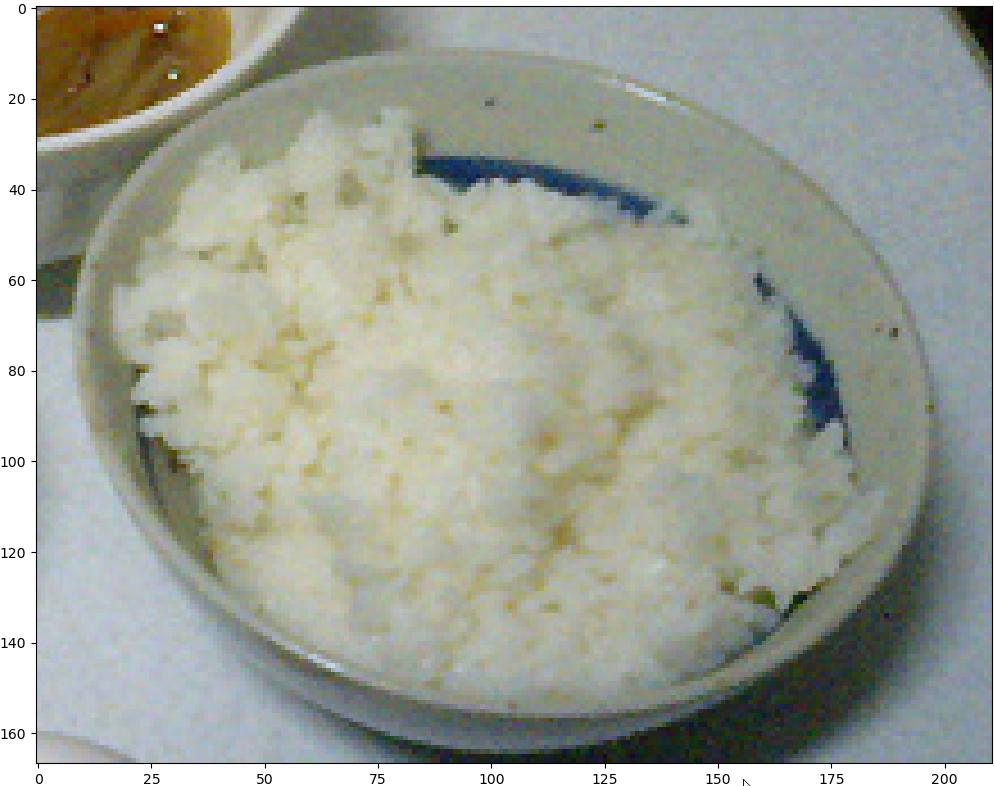
\includegraphics[width=\textwidth]{εικόνα_μετά.png}
\caption{Μετά}
\end{subfigure} 
\caption{UECFOOD256 αποκοπή εικόνας}
\label{Crop_image}
\end{figure}

Επιπλέον η ύπαρξη των bounding boxes ήταν και ο βασικός λόγος που επιλέχθηκε το συγκεκριμένο σύνολο δεδομένων ως αρχικό και όχι το FOOD101, όπως ήταν η αρχική πρόθεση, καθώς προτιμήθηκε η λογική της εκπαίδευσης του μοντέλου σε ένα "καθαρό" σύνολο δεδομένων το οποίο περιέχει περισσότερες κλάσεις αλλά παράλληλα λιγότερες εικόνες ανά κλάση, ώστε να εκτεθεί το μοντέλο σε πολλά διαφορετικά είδη τροφών και να αναπτύξει με αυτό τον τρόπο τη δυνατότητα να εντοπίζει συγκεκριμένα χαρακτηριστικά στοιχεία (features), τα οποία και θα μπορούσαν να χρησιμοποιηθούν σε ένα άλλο σύνολο δεδομένων για την ταξινόμηση τροφών. 

Αντίθετα στο δεύτερο σύνολο δεδομένων δεν είναι διαθέσιμα αυτά τα πλαίσια εντοπισμού και για αυτό τον λόγο δεν είναι δυνατή η απομόνωση και αποκοπή της εικόνας του φαγητού, ενώ αναφέρεται ότι έχει γίνει και λανθασμένη απόδοση κλάσης σε μερικές από τις εικόνες, πράγμα που επηρεάζει αρνητικά το τελικό αποτέλεσμα.

Ένα ακόμη στοιχείο που αξίζει σχολιασμού είναι ότι η προ-επεξεργασία των εικόνων είναι μια αρκετά χρονοβόρα διαδικασία η οποία ξεπερνάει τη μια ώρα για κάθε σύνολο δεδομένων, οπότε επελέγη οι εικόνες να επεξεργαστούν μια φορά για κάθε επιλεγόμενη διάσταση πχ (128, 128) και να αποθηκευτούν σε αρχεία τύπου .h5. Στη συνέχεια κάθε φορά που το πρόγραμμα εκτελείτο οι εικόνες διαβάζονταν απευθείας από τα αρχεία και εισάγονταν στο πρόγραμμα ως πίνακες (numpy.arrays) τύπου int8.

Τέλος μετά την προ-επεξεργασία και αποθήκευση των εικόνων γίνεται ο διαχωρισμός των δεδομένων σε training-validation-test set με αναλογίες 70\%-15\%-15\% και είναι πλέον δυνατή η εκτέλεση του επόμενου βήματος που αφορά την εκπαίδευση του νευρωνικού δικτύου. 
\chapter{Εκπαίδευση μοντέλων}
\thispagestyle{empty} % We remove page numbering
\vspace{-2em}
\section{Αρχιτεκτονικές}
\label{ArchitecturesUsed}

Με την ολοκλήρωση της προ-επεξεργασίας των εικόνων είναι εφικτό να προχωρήσει  η εκπαίδευση των διαφόρων μοντέλων ταξινομητών για το πρώτο σύνολο δεδομένων. Λόγω της φύσης του προβλήματος και τη χρήση νευρωνικών δικτύων, κάθε εποχή εκπαίδευσης είναι αρκετά χρονοβόρα και οι δοκιμές των διαφόρων αρχιτεκτονικών είναι εκ των πραγμάτων περιορισμένες. 

Στην παρούσα εργασία έγινε δοκιμή τεσσάρων διαφορετικών αρχιτεκτονικών, από τις οποίες η πρώτη δημιουργήθηκε από την αρχή, ενώ οι υπόλοιπες δημιουργήθηκαν ως ένα μείγμα προ-εκπαιδευμένων μοντέλων, που βασίζονταν στις γνωστές αρχιτεκτονικές VGG16, VGG19 και ResNet50, καθώς και ένα επιπλέον τμήμα συνελικτικών (CNN) και διασυνδεδεμένων (fully connected) επιπέδων (layers) τα οποία προστέθηκαν εκ των υστέρων ώστε μέσω αυτού να γίνει ο εντοπισμός των πιο λεπτομερών χαρακτηριστικών του προβλήματος. Οι δομές των αρχιτεκτονικών φαίνονται στα σχήματα \ref{C15D3net_Architecture_fig} και \ref{Pretrained_Architectures_fig} αντίστοιχα. 


\begin{figure}[H]
\centering
\begin{subfigure}[t]{0.9\textwidth}%
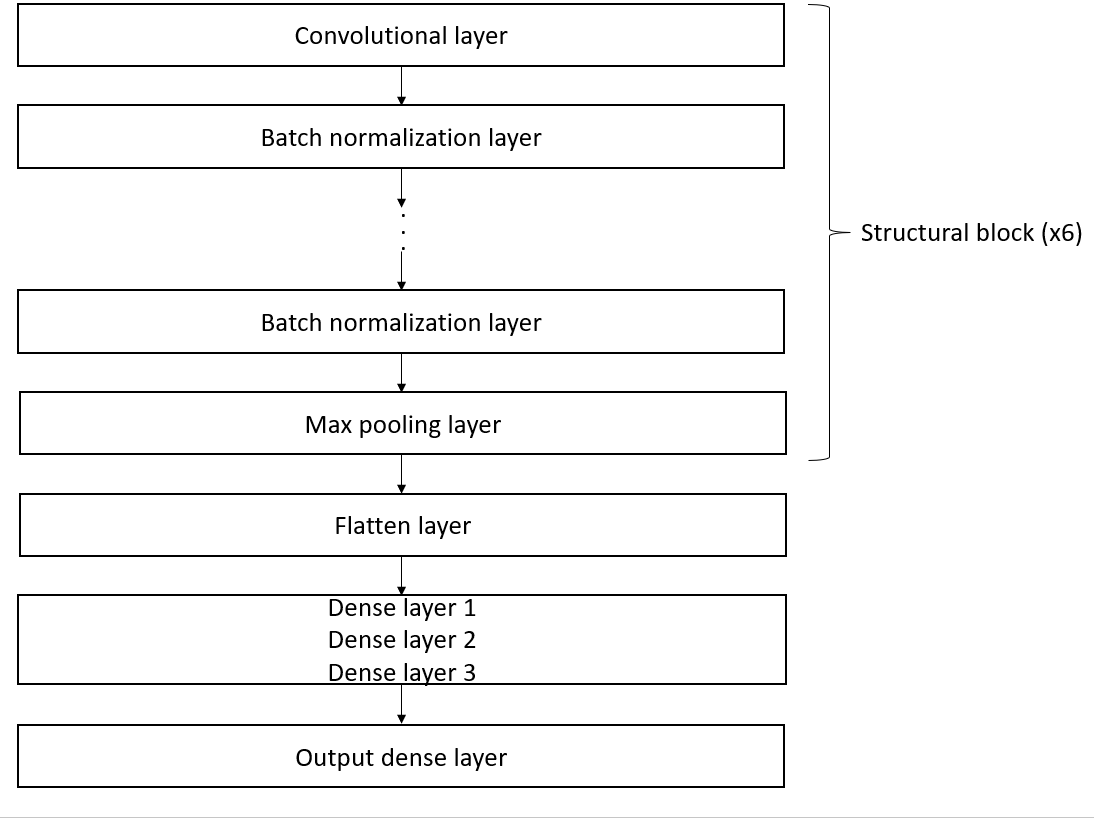
\includegraphics[width=\textwidth]{C15D3net_Architecture.png}
\end{subfigure}
\caption{Αρχικτετονική C15D3net}
\label{C15D3net_Architecture_fig}
\end{figure}

\begin{figure}[H]
\centering
\begin{subfigure}[t]{0.9\textwidth}%
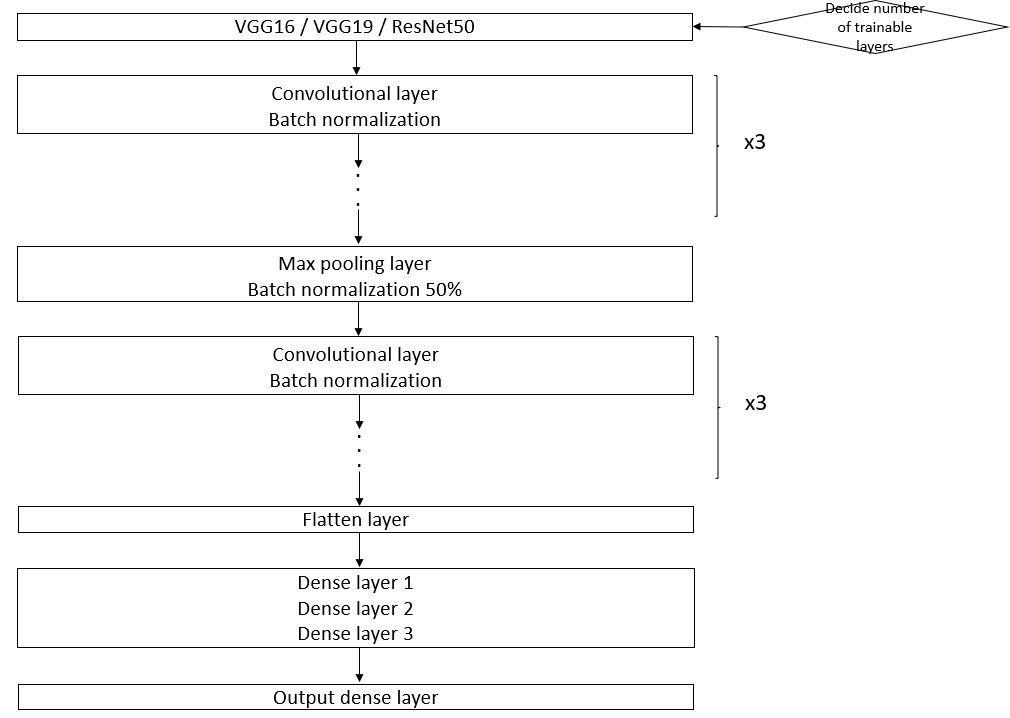
\includegraphics[width=\textwidth]{Pretrained_Architectures.png}
\end{subfigure}
\caption{Αρχικτετονικές VGG16mod, VGG19mod, ResNet50mod}
\label{Pretrained_Architectures_fig}
\end{figure}


\section{Ρύθμιση παραμέτρων}
\label{Parameters tuning}

Μετά την ανάπτυξη των διαφόρων αρχιτεκτονικών μπορεί να ακολουθήσει η διεξαγωγή δοκιμών ώστε να καταλήξουμε στο ιδανικότερο μοντέλο για την επίλυση του προβλήματος ταξινόμησης. 

Αντικειμενικός στόχος αυτών των δοκιμών ήταν η επίτευξη όσο το δυνατόν μεγαλύτερης ακρίβειας πρόβλεψης (accuracy) κατά τη διάρκεια της εκπαίδευσης, αλλά κρισιμότερα κατά την διαδικασία επαλήθευσης (validation), η οποία αποτελεί ένα καλό δείκτη της δυνατότητας γενίκευσης του αναπτυσσόμενου μοντέλου.

Έχοντας αποφασίσει, σε γενικές γραμμές, τη δομή των διαφόρων αρχιτεκτονικών, όπως παρουσιάστηκε στα σχήματα \ref{C15D3net_Architecture_fig} και \ref{Pretrained_Architectures_fig}, ακολουθεί η παρουσίαση των δοκιμών για την επιλογή της τελικής μορφής του νευρωνικού δικτύου. Οι δοκιμές αυτές μπορούν να αποδοθούν στις παρακάτω κατηγορίες.

\begin{enumerate}
\item Μέγεθος των εικόνων
\item Χρήση γεννήτριας εικόνων (image generator)
\item Χρήση regularizer L1,L2 για τη μείωση του βαθμού υπερπροσαρμογής (overfitting) στα δεδομένα
\item Επιμέρους παράμετροι εκπαίδευσης (αριθμός εποχών, είδος βελτιστοποιητή, κτλ.) για γρηγορότερη και καλύτερη σύγκλιση του μοντέλου
\item Αριθμός επιπέδων προς εκπαίδευση (trainable layers) στις αρχιτεκτονικές που χρησιμοποιούν προ-εκπαιδευμένα μοντέλα
\end{enumerate}

\begin{table}[H]
\centering
\begin{tabular}{|c|c|c|c|c|}
\hline
\diagbox{Αρχιτεκτονική}{Μέγεθος εικόνων} & (64, 64, 3) & (128, 128, 3) & (160, 160, 3) & (256, 256, 3) \\ \hline
ResNet50mod (1) & $\surd$ & $\surd$ & $\surd$ & $\surd$ \\ \hline
ResNet50mod (2) &         &         & $\surd$ &         \\ \hline
ResNet50mod (3) &         &         & $\surd$ &         \\ \hline
ResNet50mod (4) &         &         & $\surd$ &         \\ \hline
VGG16mod        &         &         & $\surd$ &         \\ \hline
VGG19mod        &         &         & $\surd$ &         \\ \hline
C15D3net        &         &         & $\surd$ &         \\ \hline
\end{tabular}
\caption{Περιπτώσεις αρχιτεκτονικών που ελέγχθηκαν}
\label{Tuning_Architectures_table}
\end{table}


Στον πίνακα \ref{Tuning_Architectures_table} παρουσιάζονται οι περιπτώσεις για τις οποίες πραγματοποιήθηκε εκτέλεση του κώδικα. Για τις αρχιτεκτονικές που παρουσιάζονται στην πρώτη στήλη του πίνακα και οι οποίες θα αναφερθούν λεπτομερέστερα παρακάτω ισχύουν τα εξής.

\begin{itemize}
\item ResNet50mod (1) : 20 προ-εκπαιδευμένα layers της ResNet50 προς εκπαίδευση, χωρίς εφαρμογή L1/L2 regularization, με χρήση γεννήτριας εικόνων
\item ResNet50mod (2) : 20 προ-εκπαιδευμένα layers της ResNet50 προς εκπαίδευση, χωρίς εφαρμογή L1/L2 regularization, χωρίς χρήση γεννήτριας εικόνων
\item ResNet50mod (3) : 20 προ-εκπαιδευμένα layers της ResNet50 προς εκπαίδευση, με χρήση L1/L2 regularization, με χρήση γεννήτριας εικόνων
\item ResNet50mod (4) : 0 προ-εκπαιδευμένα layers της ResNet50 προς εκπαίδευση, χωρίς εφαρμογή L1/L2 regularization, με χρήση γεννήτριας εικόνων
\item VGG16mod : 0 προ-εκπαιδευμένα layers της VGG16 προς εκπαίδευση, χωρίς εφαρμογή L1/L2 regularization, με χρήση γεννήτριας εικόνων
\item VGG19mod : 0 προ-εκπαιδευμένα layers της VGG19 προς εκπαίδευση, χωρίς εφαρμογή L1/L2 regularization, με χρήση γεννήτριας εικόνων
\item C15D3net : Αρχιτεκτονική που αναπτύχθηκε εξ'αρχής. Αποτελείται από 15 συνελικτικά και 3 πλήρως διασυνδεδεμένα επίπεδα 
\end{itemize}

\subsubsection{Μέγεθος εικόνων}

Αρχικά, η πρώτη παράμετρος που πρέπει να καθοριστεί είναι το μέγεθος των εικόνων που θα χρησιμοποιηθούν κατά την εκπαίδευση. Πρόκειται για μια πολύ σημαντική παράμετρο της οποίας η τιμή επιλέγεται πριν αρχίσει η διαδικασία εκπαίδευσης, κατά το στάδιο της προ-επεξεργασίας εικόνων, αλλά έχει σημαντικές συνέπειες για την πολυπλοκότητα, την τελική ακρίβεια του μοντέλου αλλά και τη δυνατότητα εκπαίδευσης του μοντέλου λόγω επάρκειας μνήμης όπως και τον χρόνο εκπαίδευσης. 

Στο σχήμα \ref{image_compare_sizes_training} φαίνεται η ακρίβεια που επιτυγχάνεται κατά τη διάρκεια εκπαίδευσης για την ίδια ακριβώς αρχιτεκτονική, η οποία είναι η τροποποιημένη ResNet50 με 20 trainable layers και χωρίς τη χρήση regularizer, δηλαδή η περίπτωση ResNet50mod (1) που αναφέραμε πιο πάνω, για τέσσερις διαφορετικές διαστάσεις εικόνων (64, 64, 3) (128, 128, 3), (160, 160, 3) και (256, 256, 3).


Στο σχήμα \ref{image_compare_sizes_validation}, φαίνονται οι τιμές κατά την διαδικασία της επαλήθευσης. Επιπλέον στον πίνακα \ref{Different_sizes_same_architecture_table} παρουσιάζεται συγκεντρωτικά ο αριθμός των παραμέτρων προς εκπαίδευση για κάθε μια από αυτές τις περιπτώσεις, αλλά και για όλες τις υπόλοιπες περιπτώσεις τις οποίες μελετήσαμε.

\begin{figure}[H]
\centering
\begin{subfigure}[t]{0.49\textwidth}
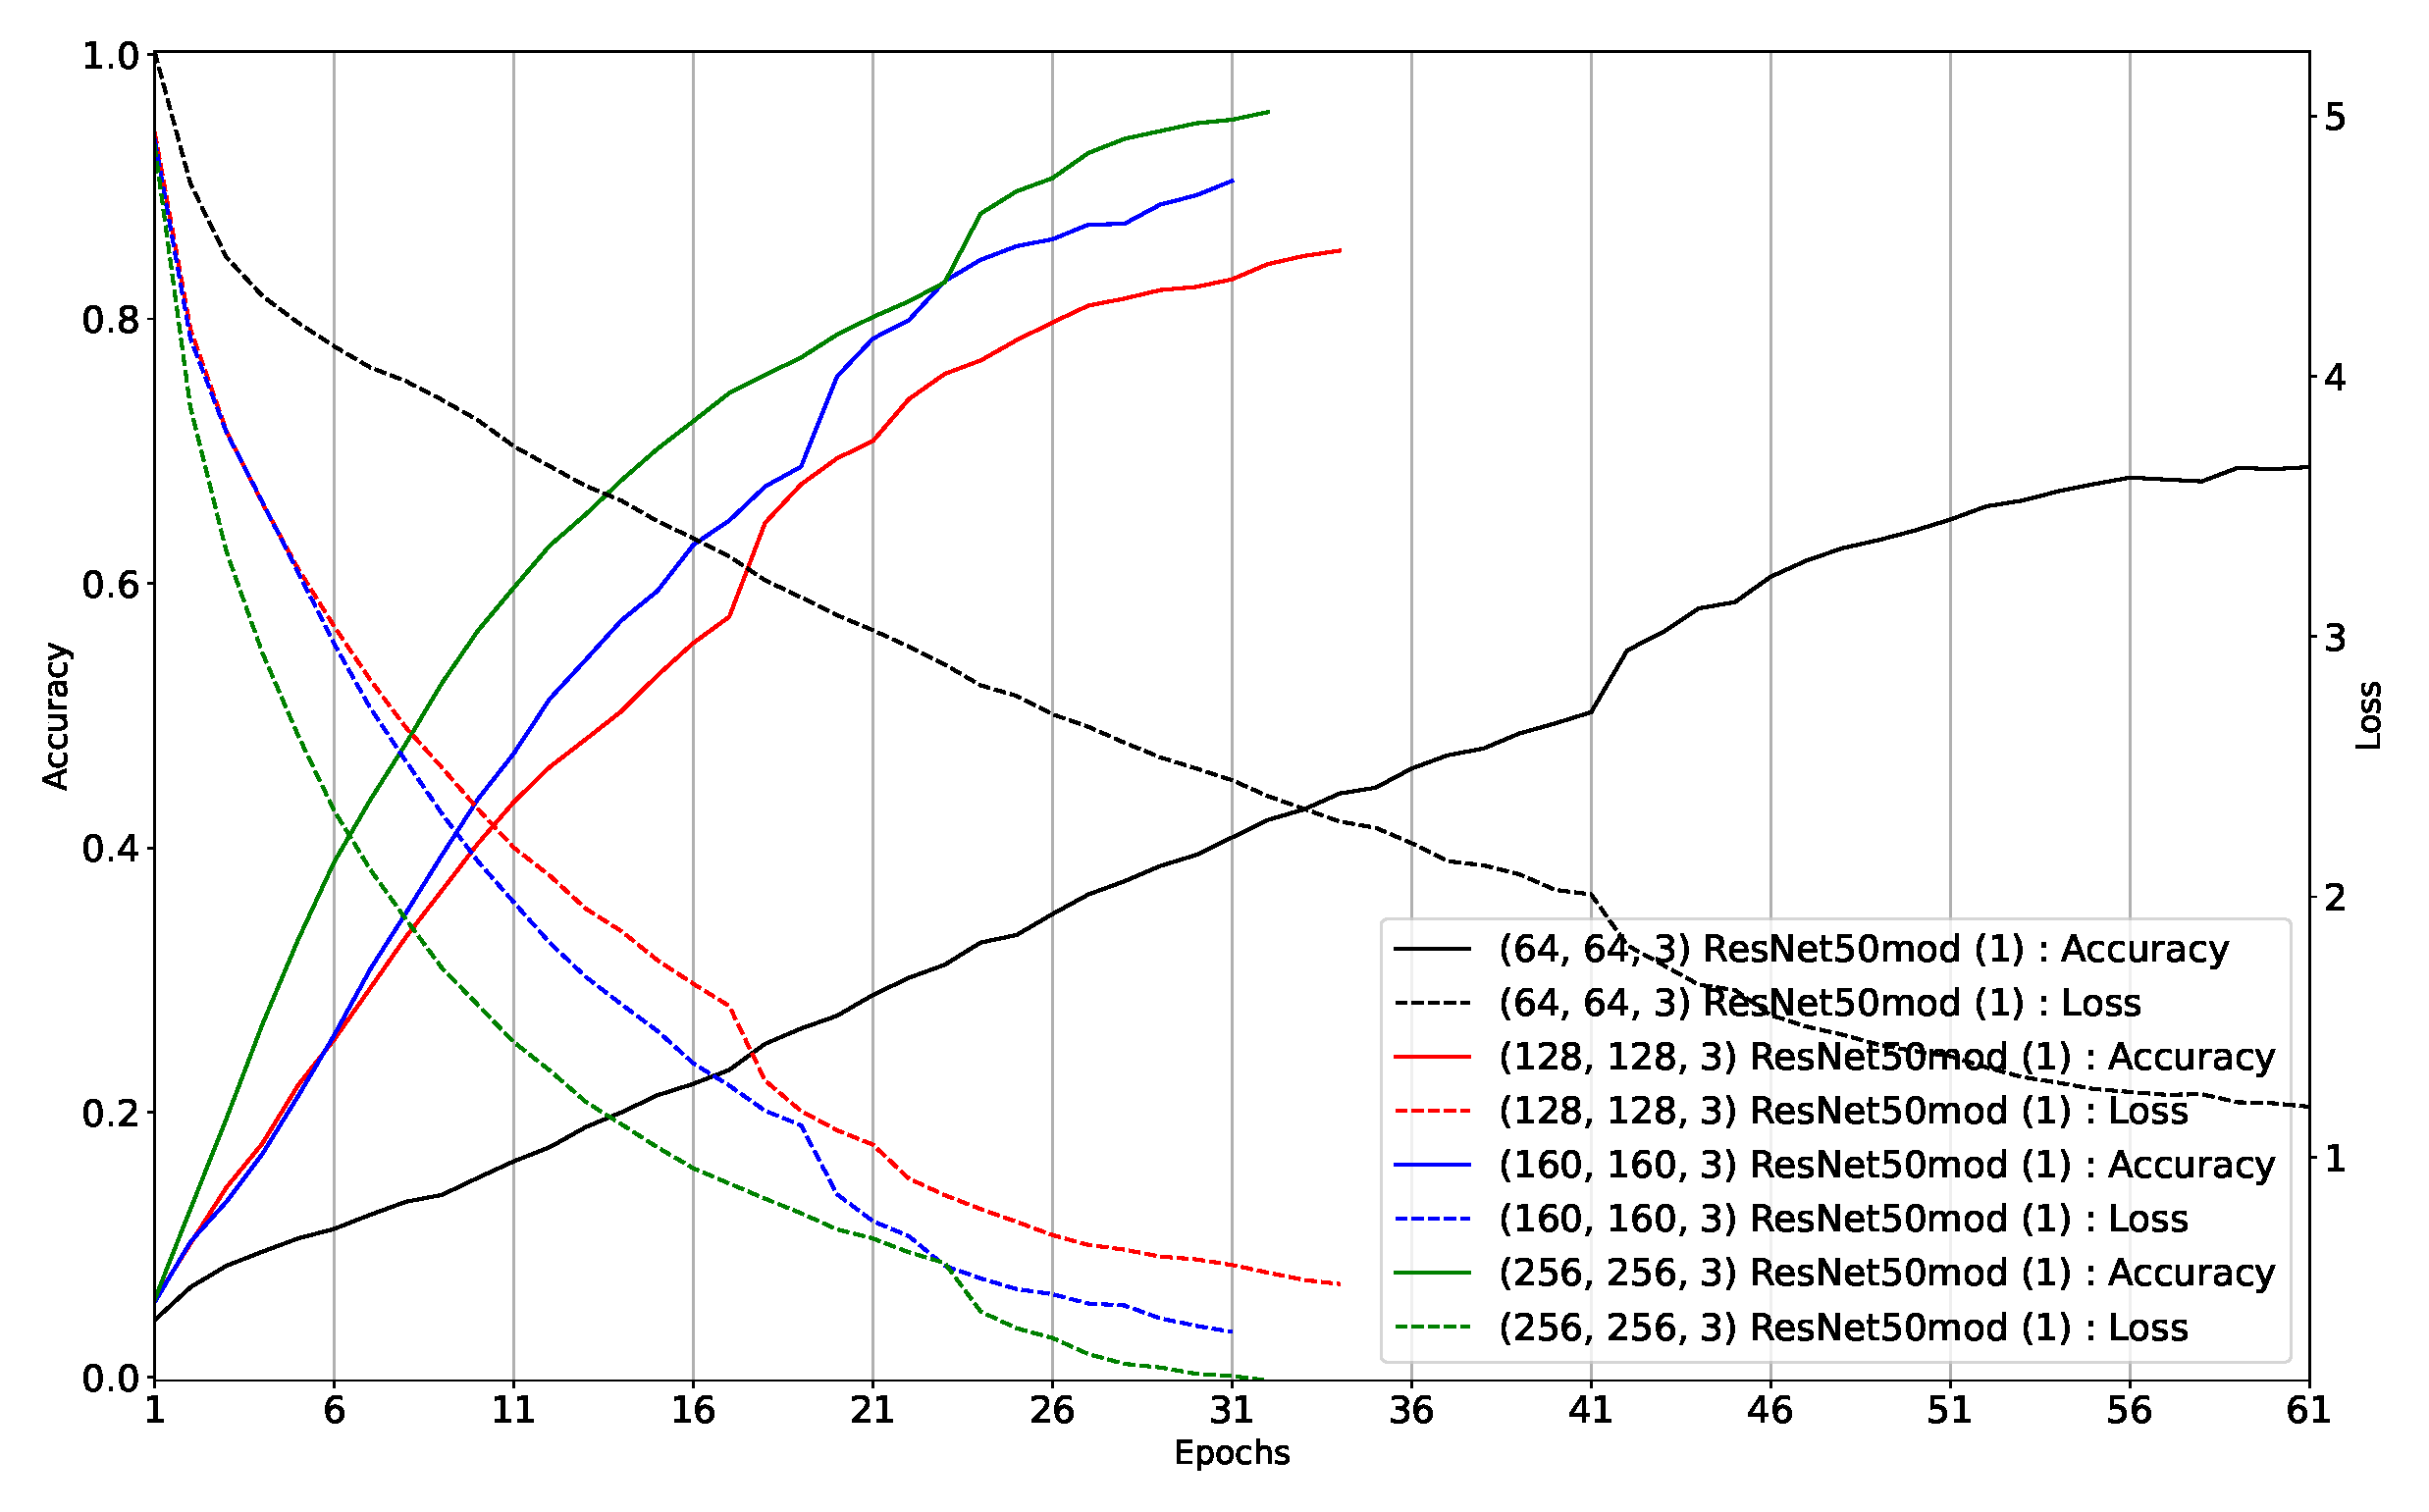
\includegraphics[width=\textwidth]{History_Compare_Sizes_Training.pdf}
\caption{Training}
\label{image_compare_sizes_training}
\end{subfigure}
\begin{subfigure}[t]{0.49\textwidth}
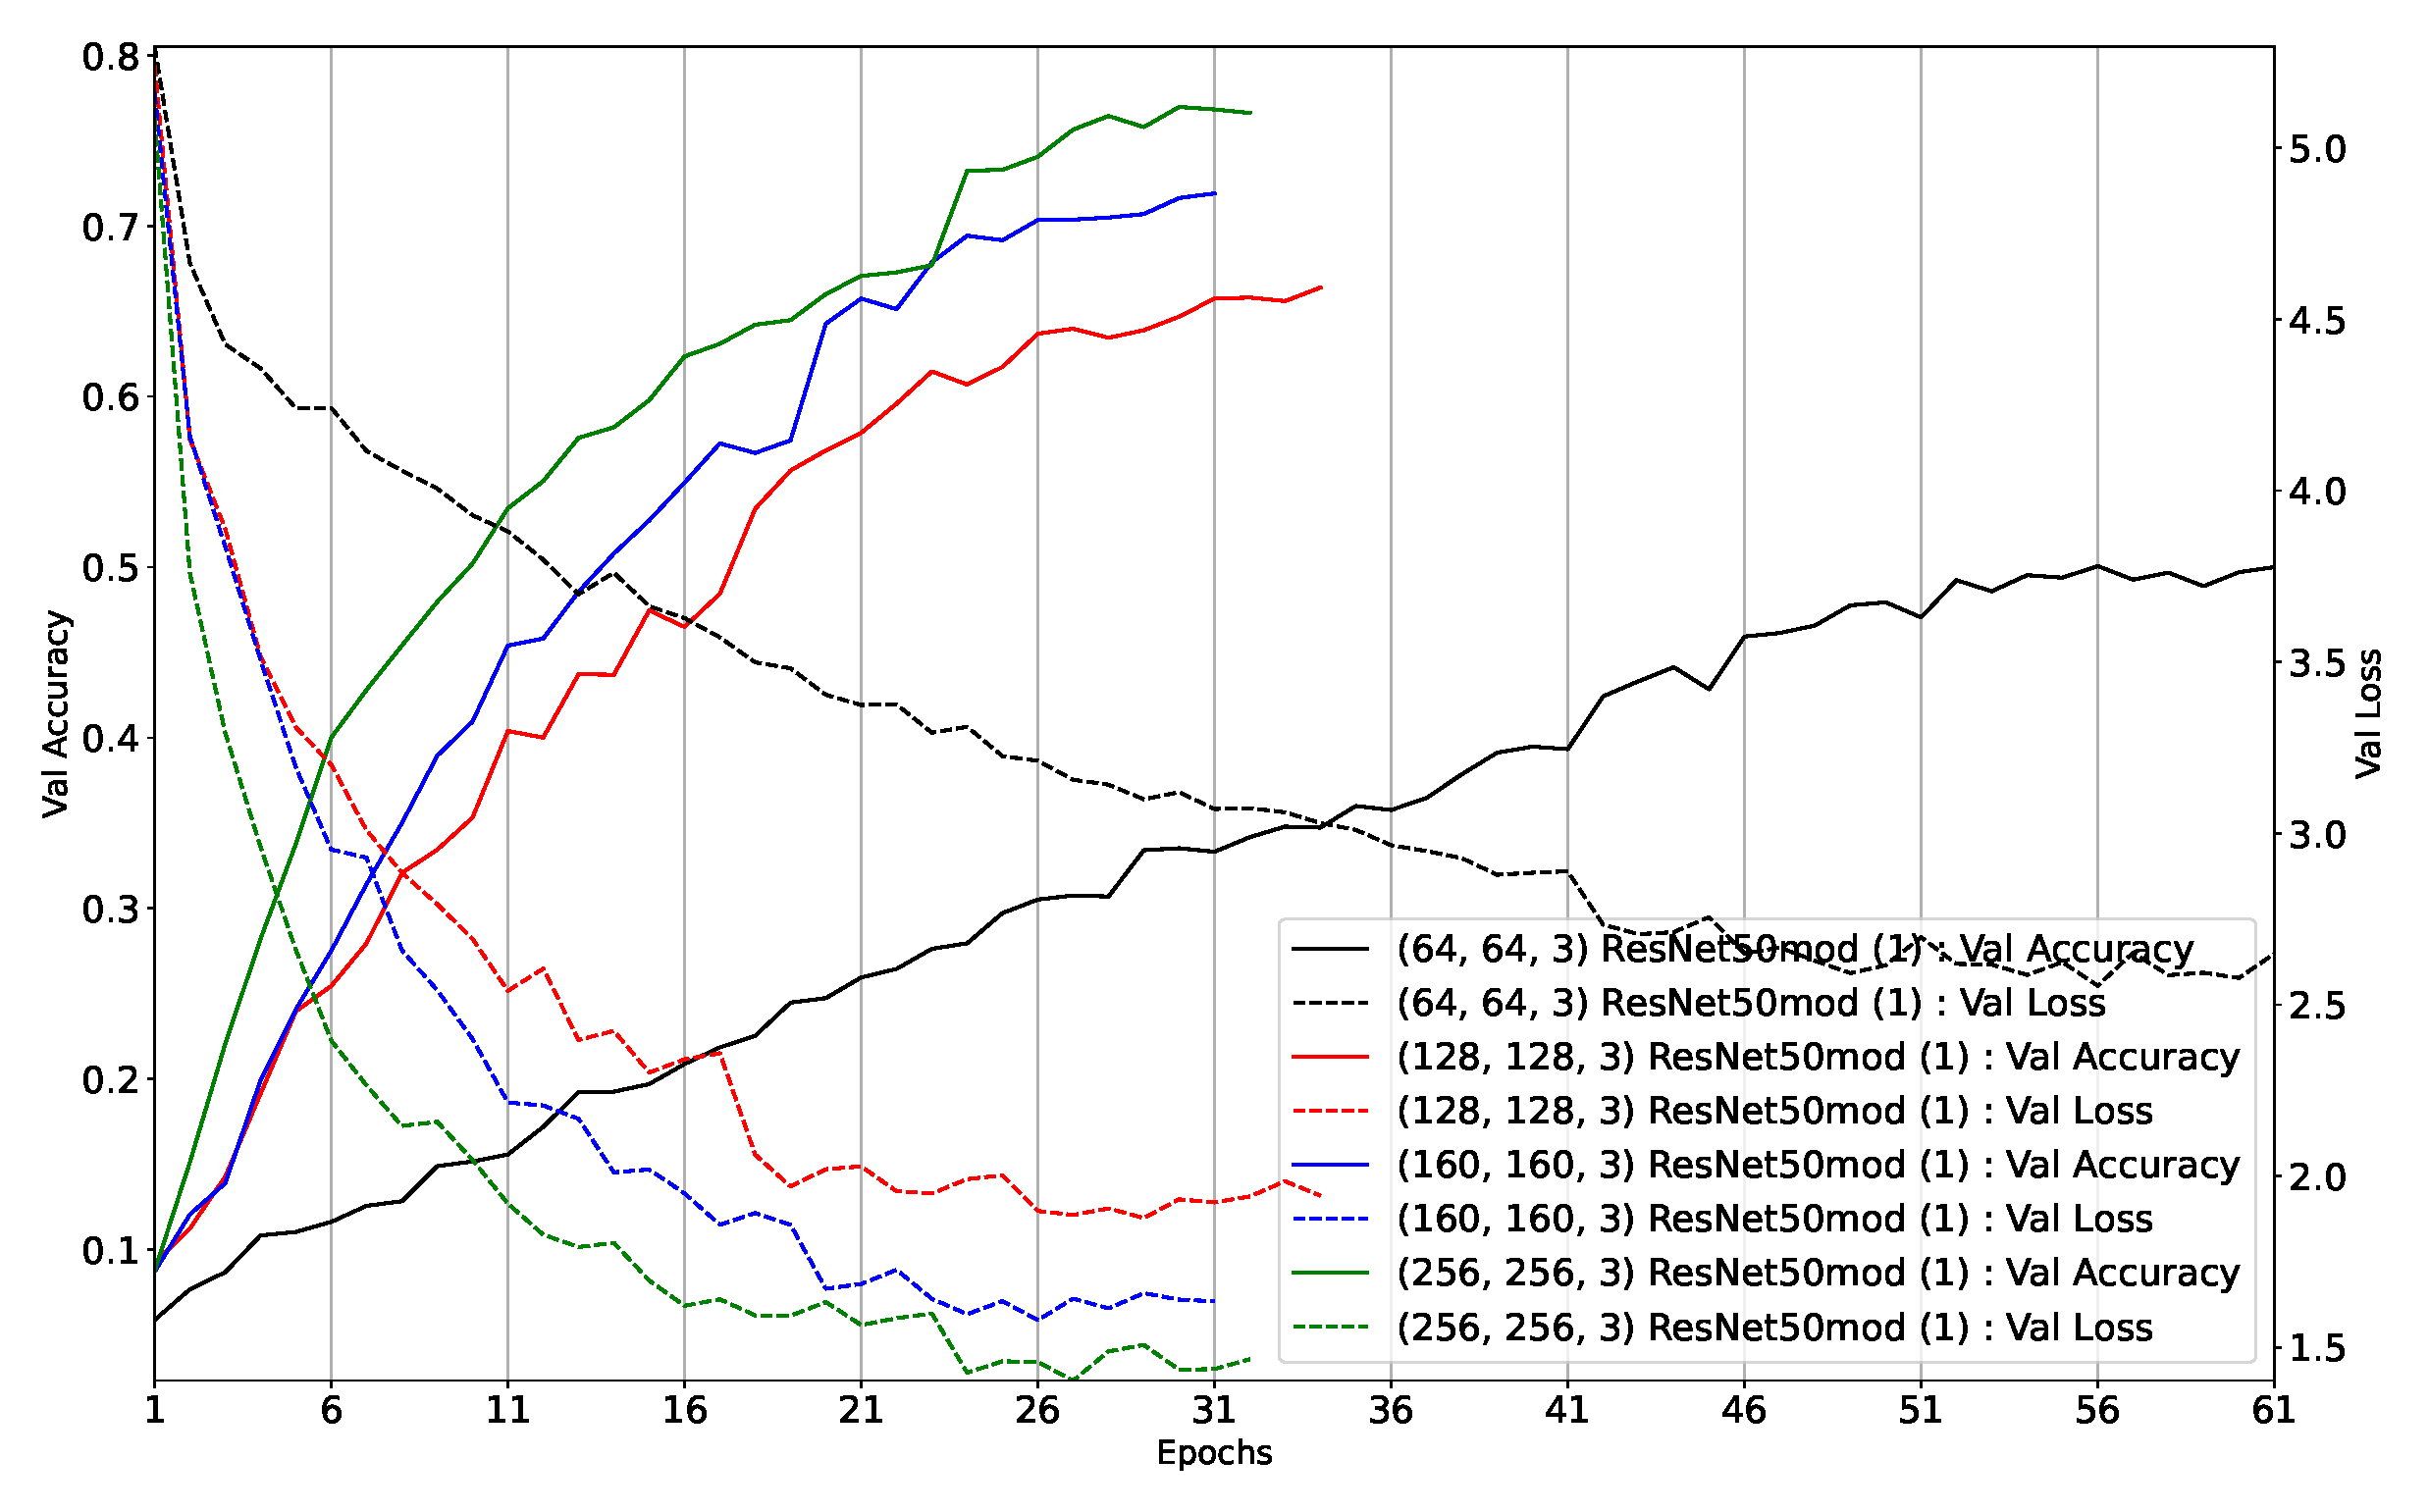
\includegraphics[width=\textwidth]{History_Compare_Sizes_Validation.pdf}
\caption{Validation}
\label{image_compare_sizes_validation}
\end{subfigure}
\caption{Επίδραση μεγέθους εικόνας}
\label{Different_sizes_same_architecture_fig}
\end{figure}

\begin{table}[H]
\centering
\begin{tabular}{|c|c|c|c|c|}
\hline
\diagbox{Αρχιτεκτονική}{Μέγεθος εικόνων}  & (64, 64, 3) & (128, 128, 3) & (160, 160, 3) & (256, 256, 3) \\ \hline
ResNet50mod (1) & 30,221,728 & 30,477,888 & 30,561,424 & 32,403,328  \\ \hline
ResNet50mod (2) &            &            & 30,561,424 &             \\ \hline
ResNet50mod (3) &            &            & 30,561,424 &             \\ \hline
ResNet50mod (4) &            &            & 21,630,096 &             \\ \hline
VGG16mod        &            &            & 7,423,621  &             \\ \hline
VGG19mod        &            &            & 7,423,621  &             \\ \hline
C15D3net        &            &            & 6,114,716  &             \\ \hline
\end{tabular}
\caption{Αριθμός παραμέτρων προς εκπαίδευση}
\label{Different_sizes_same_architecture_table}
\end{table}

Όπως είναι φανερό από τον πίνακα \ref{Different_sizes_same_architecture_table} η χρήση μεγαλύτερων σε μέγεθος εικόνων δεν αυξάνει ιδιαίτερα τον αριθμό των προς εκπαίδευση παραμέτρων, αλλά το σχήμα \ref{Different_sizes_same_architecture_fig} καταδεικνύει ότι η ακρίβεια που επιτυγχάνει το μοντέλο τόσο κατά την εκπαίδευση όσο και κατά την επαλήθευση βελτιώνεται με την αύξηση του μεγέθους, ενώ αντίθετα η συνάρτηση κόστους βαίνει διαρκώς μειούμενη. Αυτό μπορεί να εξηγηθεί από το γεγονός ότι οι μεγαλύτερες σε μέγεθος εικόνες περιέχουν περισσότερες λεπτομέρειες οι οποίες μπορούν να εντοπιστούν κατά την εκπαίδευση του νευρωνικού δικτύου.

Από την παραπάνω ανάλυση θα περίμενε κανείς να επιλεγούν για την συνέχεια των δοκιμών η χρήση εικόνων (256, 256, 3). Όμως για την σύγκριση μεταξύ μοντέλων αρκεί να έχουν εκπαιδευτεί όλα με τον ίδιο μέγεθος εικόνων οπότε και προτιμήθηκε οι υπόλοιπες δοκιμές να γίνουν με εικόνες διαστάσεων (160, 160, 3).

\subsubsection{Γεννήτρια εικόνων}

Ένα άλλο πολύ σημαντικό στοιχείο για την αποτελεσματική εκπαίδευση του νευρωνικού δικτύου είναι η χρήση γεννήτριας εικόνων (image generator). Πρόκειται επί της ουσίας για μια συνάρτηση βιβλιοθήκης της python η οποία πραγματοποιεί αλλαγές στις εικόνες που χρησιμοποιούνται κατά την εκπαίδευση αλλά και την επαλήθευση. Λόγω της διαφοροποίησης των εικόνων εισόδου, αναμένεται μείωση του βαθμού υπερπροσαρμογής αλλά και αυξημένη ακρίβεια πρόβλεψης, το οποίο επιβεβαιώνεται στο σχήμα \ref{image_generator_fig}. 

Πιο αναλυτικά στο σχήμα \ref{image_generator_training} το οποίο αναπαριστά την εξέλιξη των τιμών της ακρίβειας και της συνάρτησης κόστους κατά την εκπαίδευση, βλέπουμε ότι και στις δύο περιπτώσεις, με και χωρίς τη χρήση γεννήτριας αριθμών τα αποτελέσματα, είναι παραπλήσια. Το ενδιαφέρον στοιχείο όμως εμφανίζεται από την παρατήρηση του σχήματος \ref{image_generator_validation}, όπου όπως και προηγουμένως παρουσιάζεται η ιστορία εξέλιξης της ακρίβειας και της συνάρτησης κόστους για το σύνολο δεδομένων επαλήθευσης. Γίνεται εμφανές παρατηρώντας τις μαύρες καμπύλες, ότι σχετικά γρήγορα κατά τη διάρκεια της εκπαίδευσης χωρίς τη χρήση γεννήτριας εικόνων, το μοντέλο οδηγείται σε υπερπροσαρμογή, καθώς η συνάρτηση κόστους αυξάνει την τιμή και αντίστοιχα η επιτυγχανόμενη ακρίβεια είναι πολύ μικρότερη της ακρίβειας του μοντέλου με χρήση image generator. 

Τέλος, στον πίνακα \ref{image_generator_table} φαίνονται τα όρια των επιτρεπόμενων αλλαγών στις εικόνες. Αυτά επιλέχθηκαν με χρήση πολύ λίγων επαναλήψεων και πιθανώς μια συστηματικότερη εξέταση των δυνατών τιμών τους να οδηγούσε σε μικρή βελτίωση των αποτελεσμάτων.


\begin{figure}[H]
\centering
\begin{subfigure}[t]{0.49\textwidth}
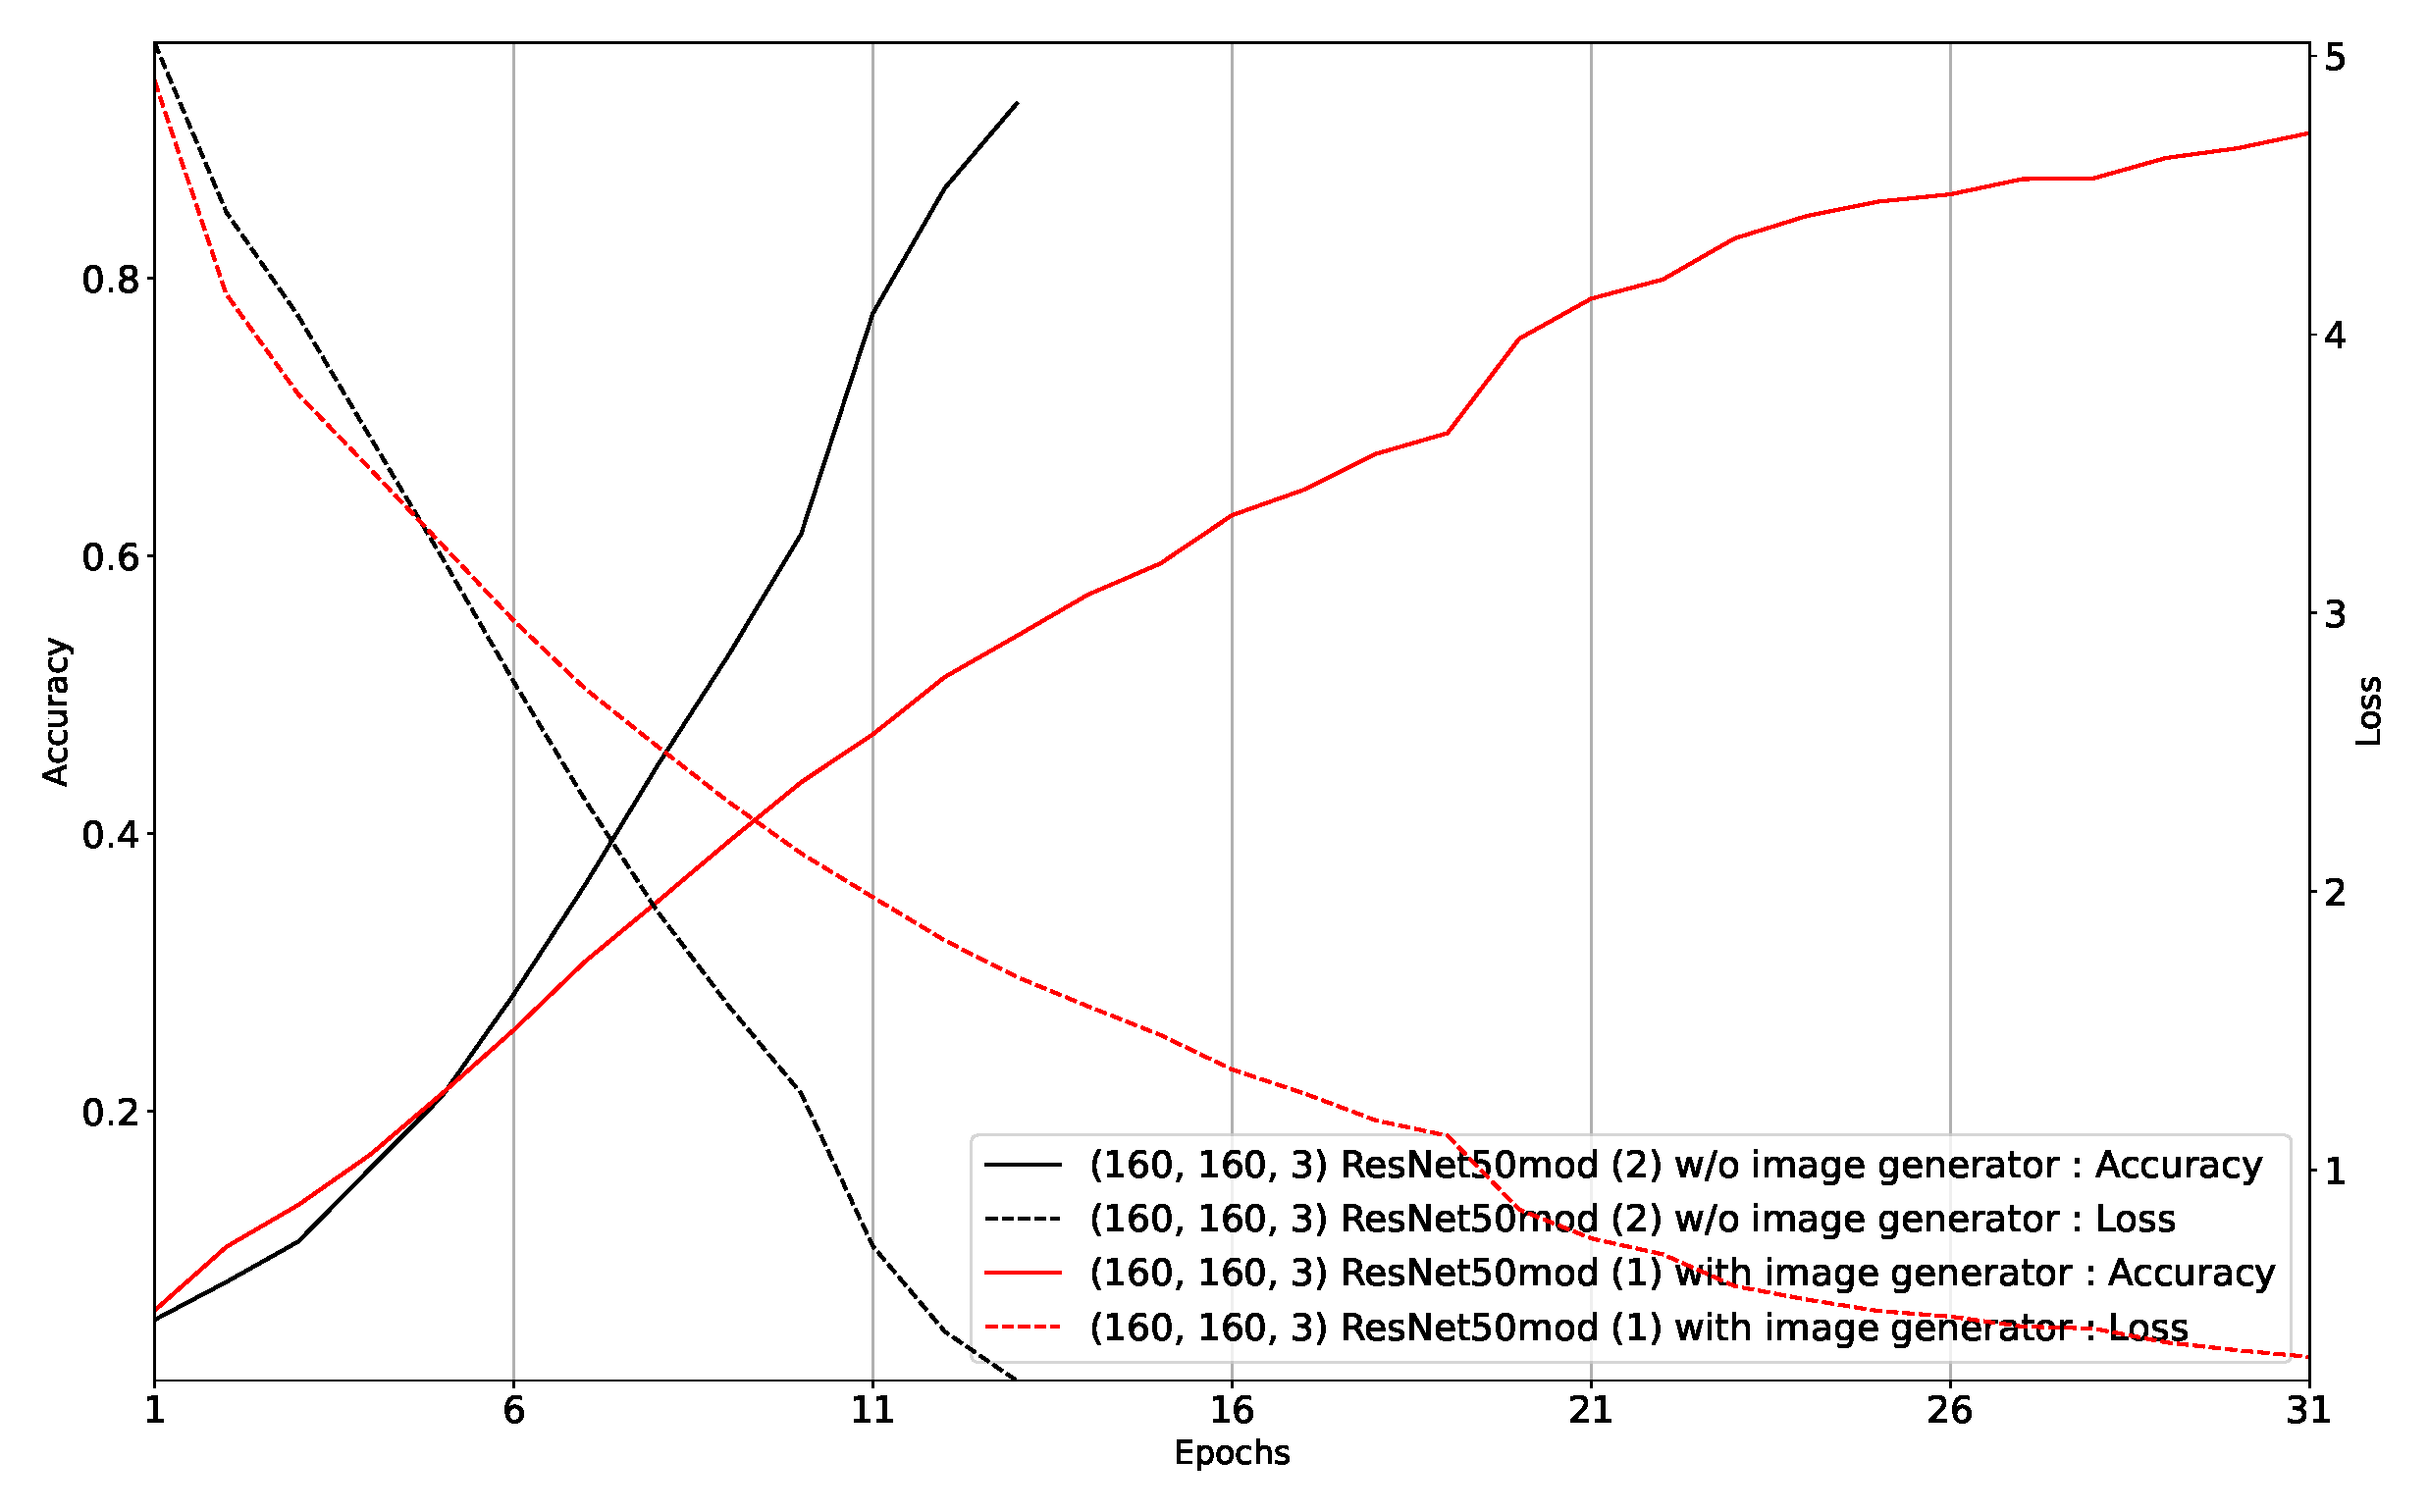
\includegraphics[width=\textwidth]{History_Compare_Generators_Training.pdf}
\caption{Training}
\label{image_generator_training}
\end{subfigure}
\begin{subfigure}[t]{0.49\textwidth}
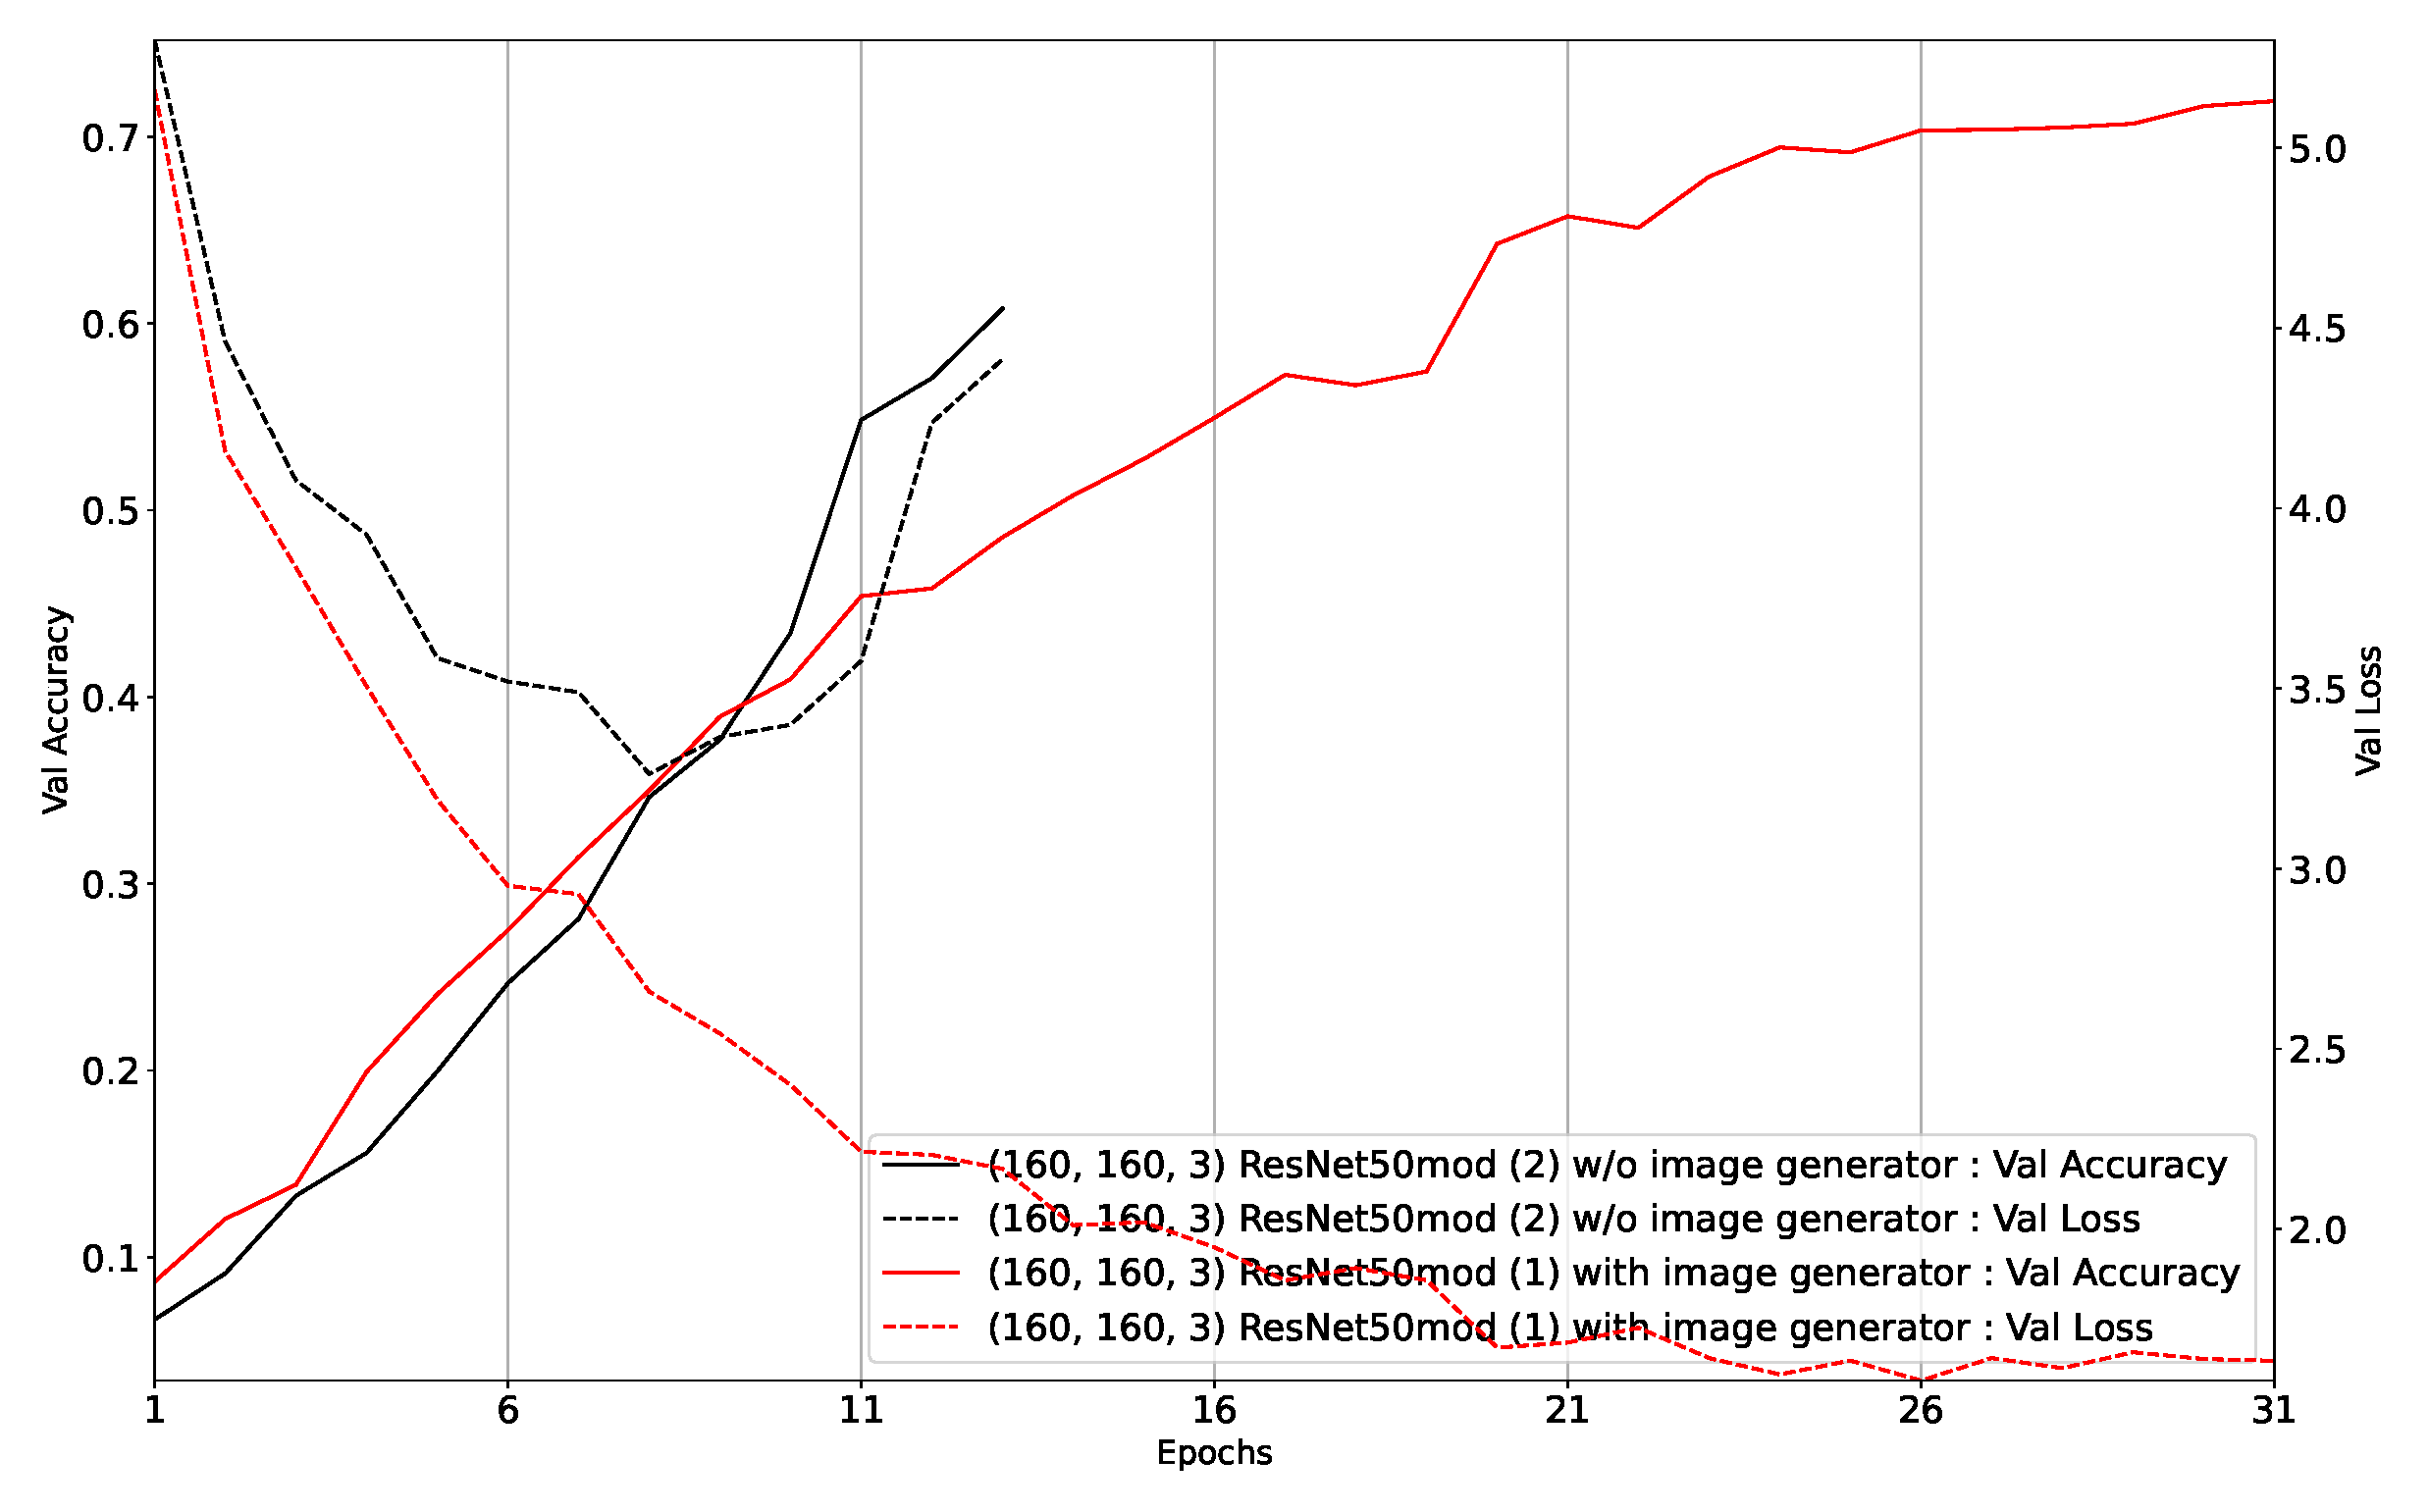
\includegraphics[width=\textwidth]{History_Compare_Generators_Validation.pdf}
\caption{Validation}
\label{image_generator_validation}
\end{subfigure}
\caption{Επίδραση χρήσης γεννήτριας εικόνων}
\label{image_generator_fig}
\end{figure}


\begin{table}[H]
\centering
\begin{tabular}{|c|c|}
\hline
Παράμετρος           & Τιμή           \\ \hline
rotation\_range      & 30             \\ \hline
width\_shift\_range  & 0.1            \\ \hline
height\_shift\_range & 0.1            \\ \hline
brightness\_range    & {[}0.5, 1.0{]} \\ \hline
shear\_range         & 0.2            \\ \hline
zoom\_range          & 0.2            \\ \hline
horizontal\_flip     & True           \\ \hline
\end{tabular}
\caption{Παράμετροι image generator}
\label{image_generator_table}
\end{table}

\subsubsection{Κανονικοποίηση (Regularization)}

Μια άλλη σημαντική δοκιμή αφορά την χρήση της κανονικοποίησης των δεδομένων, μέσω της οποίας δύναται να μειωθεί η επίδραση της υπερπροσαρμογής στα νευρωνικά δίκτυα. Λόγω του μεγάλου αριθμού των παραμέτρων προς εκπαίδευση τα νευρωνικά δίκτυα έχουν την τάση να οδηγούνται σε υπερπροσαρμογή.  Ο τρόπος με τον οποίο επιτυγχάνεται αυτό στην παρούσα εργασία είναι μέσω της χρήσης επιπέδων απόρριψης (dropout layer) και την κανονικοποίηση L1 και L2. 

Σχετικά με τα dropout layers αυτά λειτουργούν με τον ακόλουθο τρόπο. Κατά τη διάρκεια της εκπαίδευσης και πιο συγκεκριμένα κατά το βήμα της προώθησης προς τα εμπρός (forward propagation) ορισμένοι από τους νευρώνες του δικτύου απενεργοποιούνται. Έτσι το δίκτυο πρέπει να εξαρτηθεί από άλλους ενεργούς νευρώνες για την αποτελεσματικότερη μάθηση. Πρόκειται δηλαδή για μια μεθοδολογία η οποία χρησιμοποιείται για να μειώσει την ευαισθησία του μοντέλου σε συγκεκριμένα χαρακτηριστικά και να βελτιώσει τη γενίκευση του μοντέλου. 

Στην παρούσα αναφορά δεν φαίνονται οι δοκιμές που έγιναν για τον αριθμό των dropout layers αλλά και το ποσοστό των νευρώνων που απορρίπτονται. Παρόλα αυτά σε όλες τις αρχιτεκτονικές του σχήματος \ref{Pretrained_Architectures_fig} χρησιμοποιήθηκε ένα dropout layer με 50\% ποσοστό απόρριψης.

Οι μέθοδοι κανονικοποίησης L1 και L2 εισάγουν έναν όρο κανονικοποίησης στη συνάρτηση κόστους του μοντέλου, το οποίο οδηγεί σε μηδενισμό ή μείωση της τιμής κάποιων εκ των παραμέτρων του μοντέλου με αποτέλεσμα να μειώνεται η υπερπροσαρμογή του μοντέλου. 

Στο σχήμα \ref{Different_regularizer_same_architecture_fig} παρουσιάζεται η επίδραση που έχει στην ακρίβεια του μοντέλου η χρήση της κανονικοποίησης. Όπως φαίνεται η εφαρμογή που επιχειρήθηκε δεν είχε κάποιο θετικό αποτέλεσμα, καθώς φαίνεται να οδηγεί σε μικρή σχετικά υποπροσαρμογή το μοντέλο και επιπλέον να οδηγεί το μοντέλο σε περισσότερες επαναλήψεις έως ότου συγκλίνει. 

Για αυτό τον λόγο δεν επιλέχθηκε η χρήση L1, L2 regularizer στις υπόλοιπες δοκιμές και στο τελικό μοντέλο. 

\begin{figure}[H]
\centering
\begin{subfigure}[t]{0.49\textwidth}
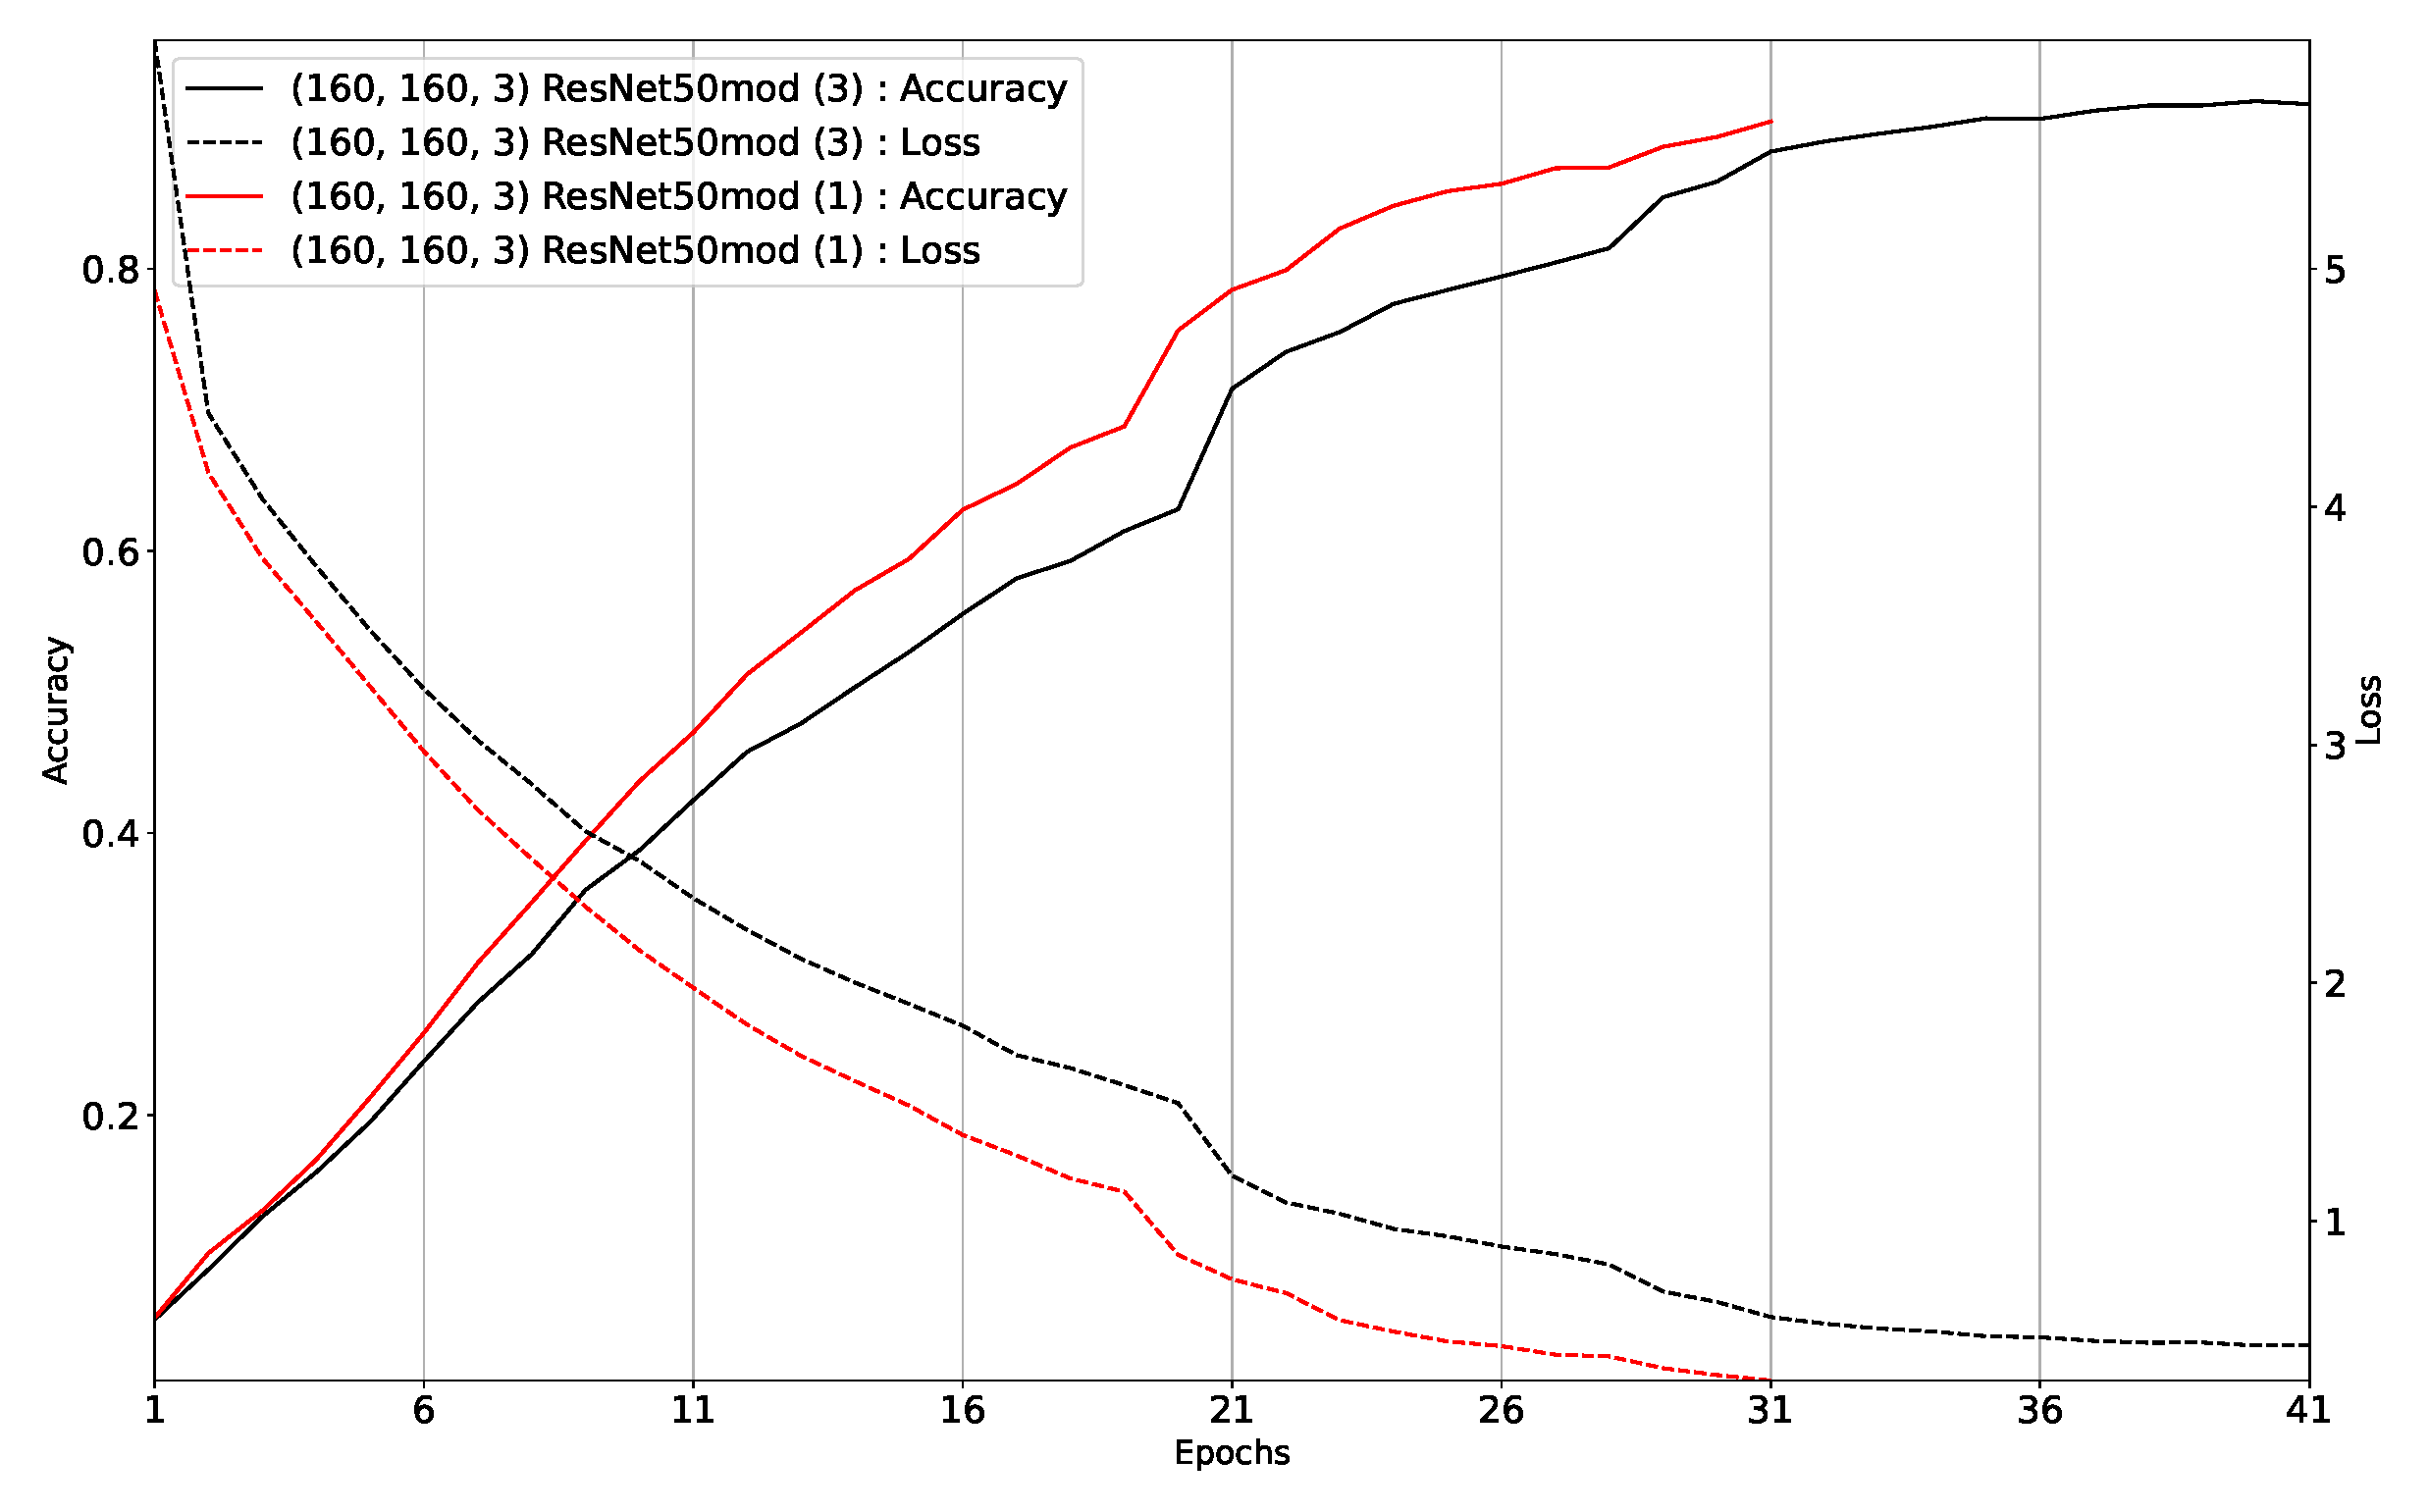
\includegraphics[width=\textwidth]{History_Compare_Regularizers_Training.pdf}
\caption{Training}
\label{image_regularizers_training}
\end{subfigure}
\begin{subfigure}[t]{0.49\textwidth}
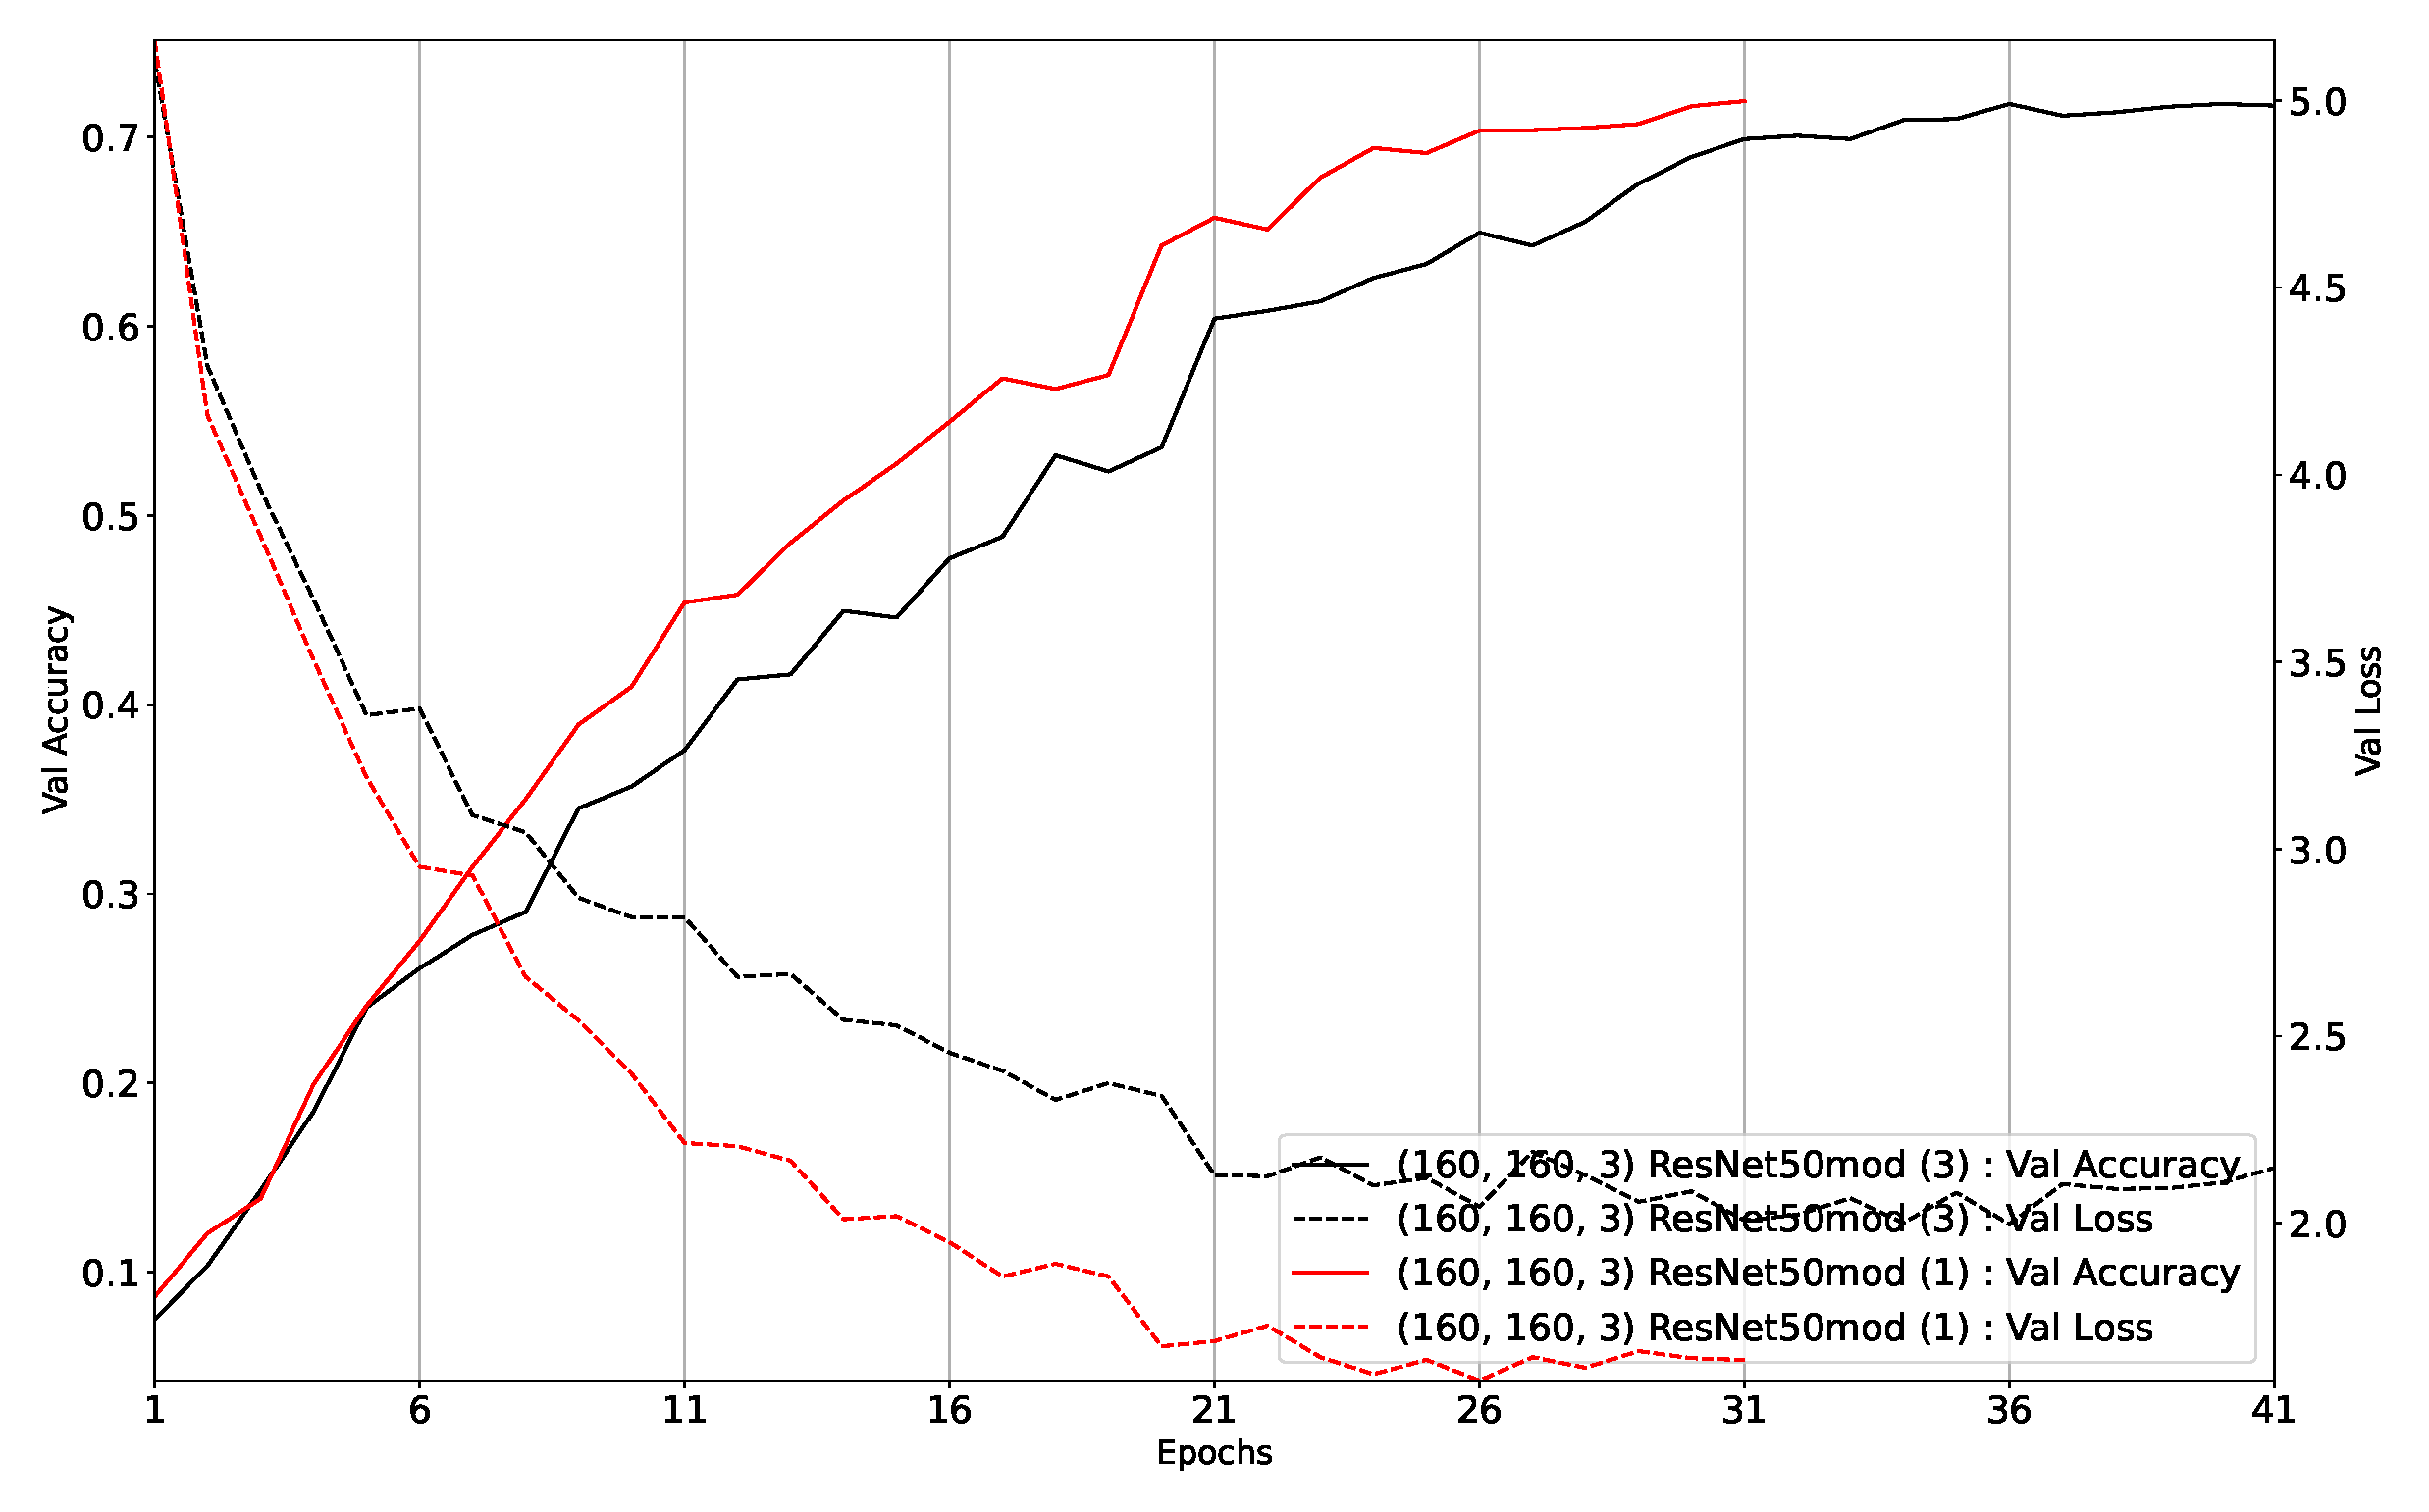
\includegraphics[width=\textwidth]{History_Compare_Regularizers_Validation.pdf}
\caption{Validation}
\label{image_regularizers_validation}
\end{subfigure}
\caption{Επίδραση χρήσης regularizer}
\label{Different_regularizer_same_architecture_fig}
\end{figure}

\subsubsection{Επιμέρους παράμετροι \& αριθμός επιπέδων προς εκπαίδευση}
Η χρήση διαφορετικών βελτιστοποιητών βρέθηκε πως δεν έχει σημαντική επίδραση στο τελικό αποτέλεσμα, αντίθετα με τον ρυθμό μάθησης (learning rate) και πιο συγκεκριμένα τον τρόπο με τον οποίο αυτός μειώνεται όταν το validation loss σταματάει να βελτιώνεται με το πέρασμα των εποχών εκπαίδευσης. 

Για να αυξήσουμε όσο το δυνατόν περισσότερο την ακρίβεια πρόβλεψης δοκιμάστηκε το ξεπάγωμα κάποιων επιπέδων στο προ-εκπαιδευμένο δίκτυο. Πρόκειται δηλαδή για την περίπτωση ResNet50mod (4), όπως αυτή αναφέρεται στους πίνακες \ref{Tuning_Architectures_table} και \ref{Different_sizes_same_architecture_table}. Στην περίπτωση του ξεπαγώματος επιπέδων όπως φαίνεται και στο σχήμα \ref{Unfreeze_Layers_fig} η αύξηση των επιπέδων προς εκπαίδευση οδηγεί σε βελτίωση της ακρίβειας το οποίο είναι αναμενόμενο από τη στιγμή που υπάρχουν περισσότερες προς εκπαίδευση παράμετροι. Πρόκειται για τη λογική που χρησιμοποιείται στο transfer learning.

\begin{figure}[H]
\centering
\begin{subfigure}[t]{0.49\textwidth}
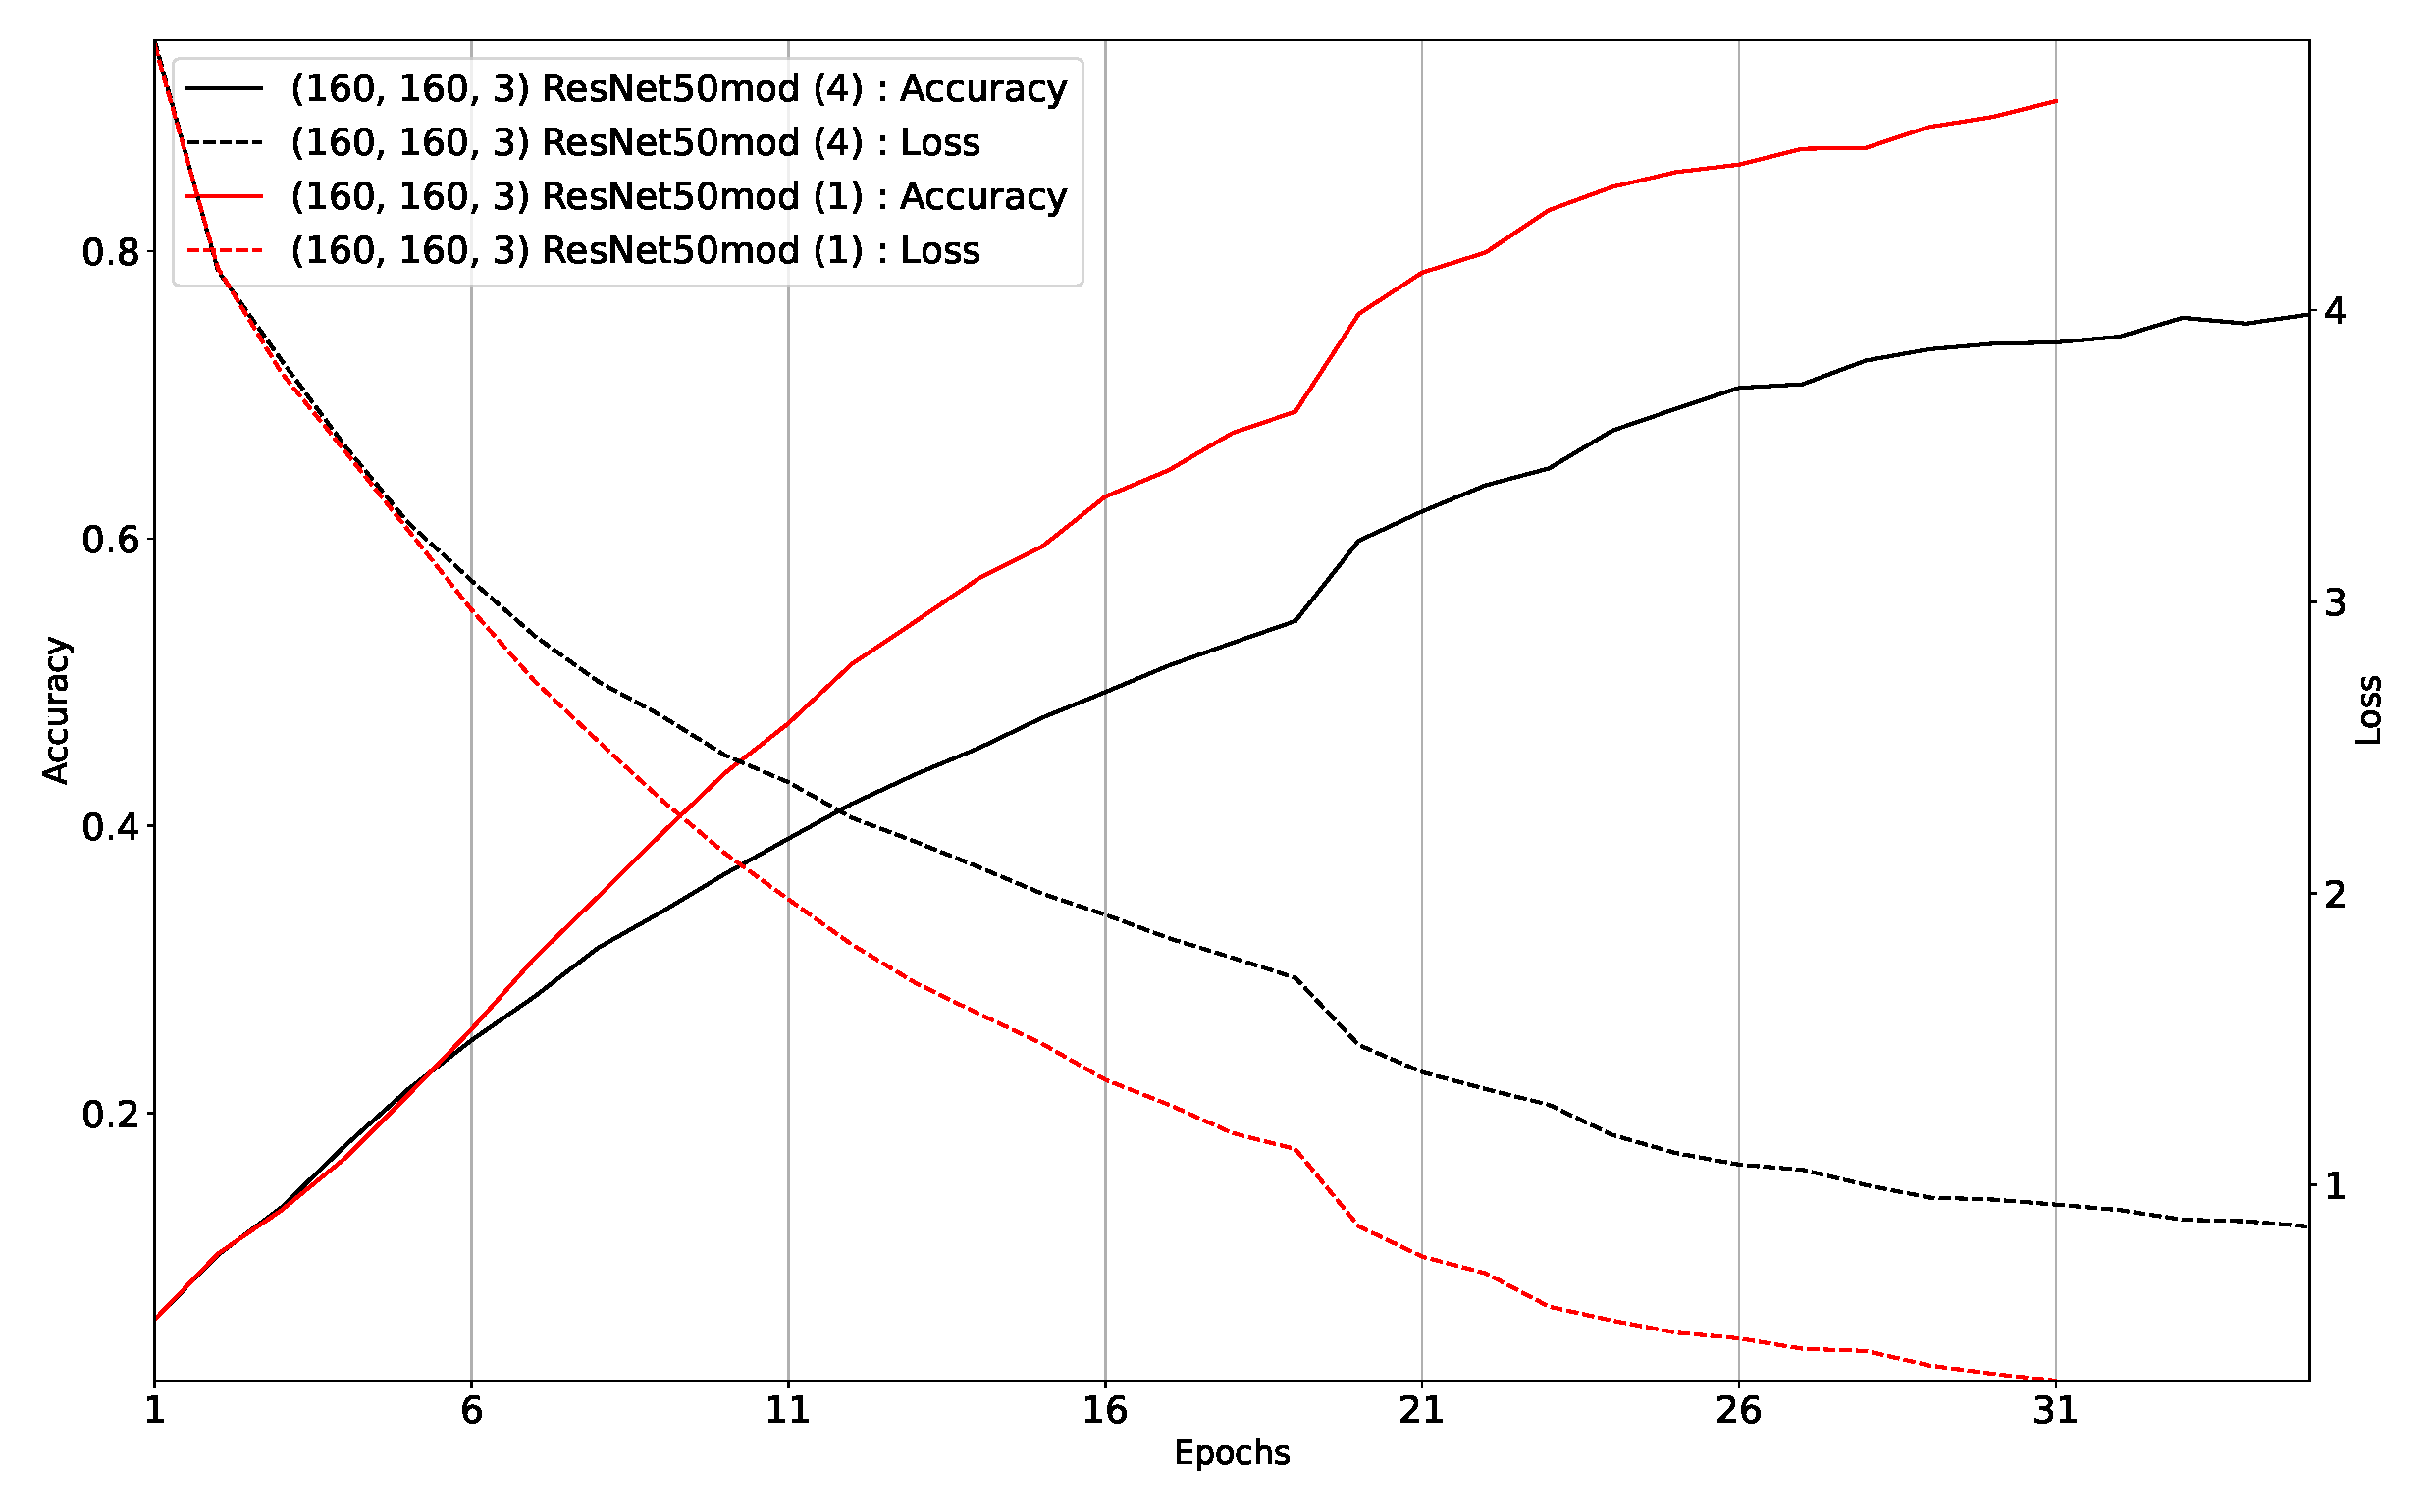
\includegraphics[width=\textwidth]{History_Compare_20unfrozen_0unfrozen_Training.pdf}
\caption{Training}
\label{image_unfrozen20_training}
\end{subfigure}
\begin{subfigure}[t]{0.49\textwidth}
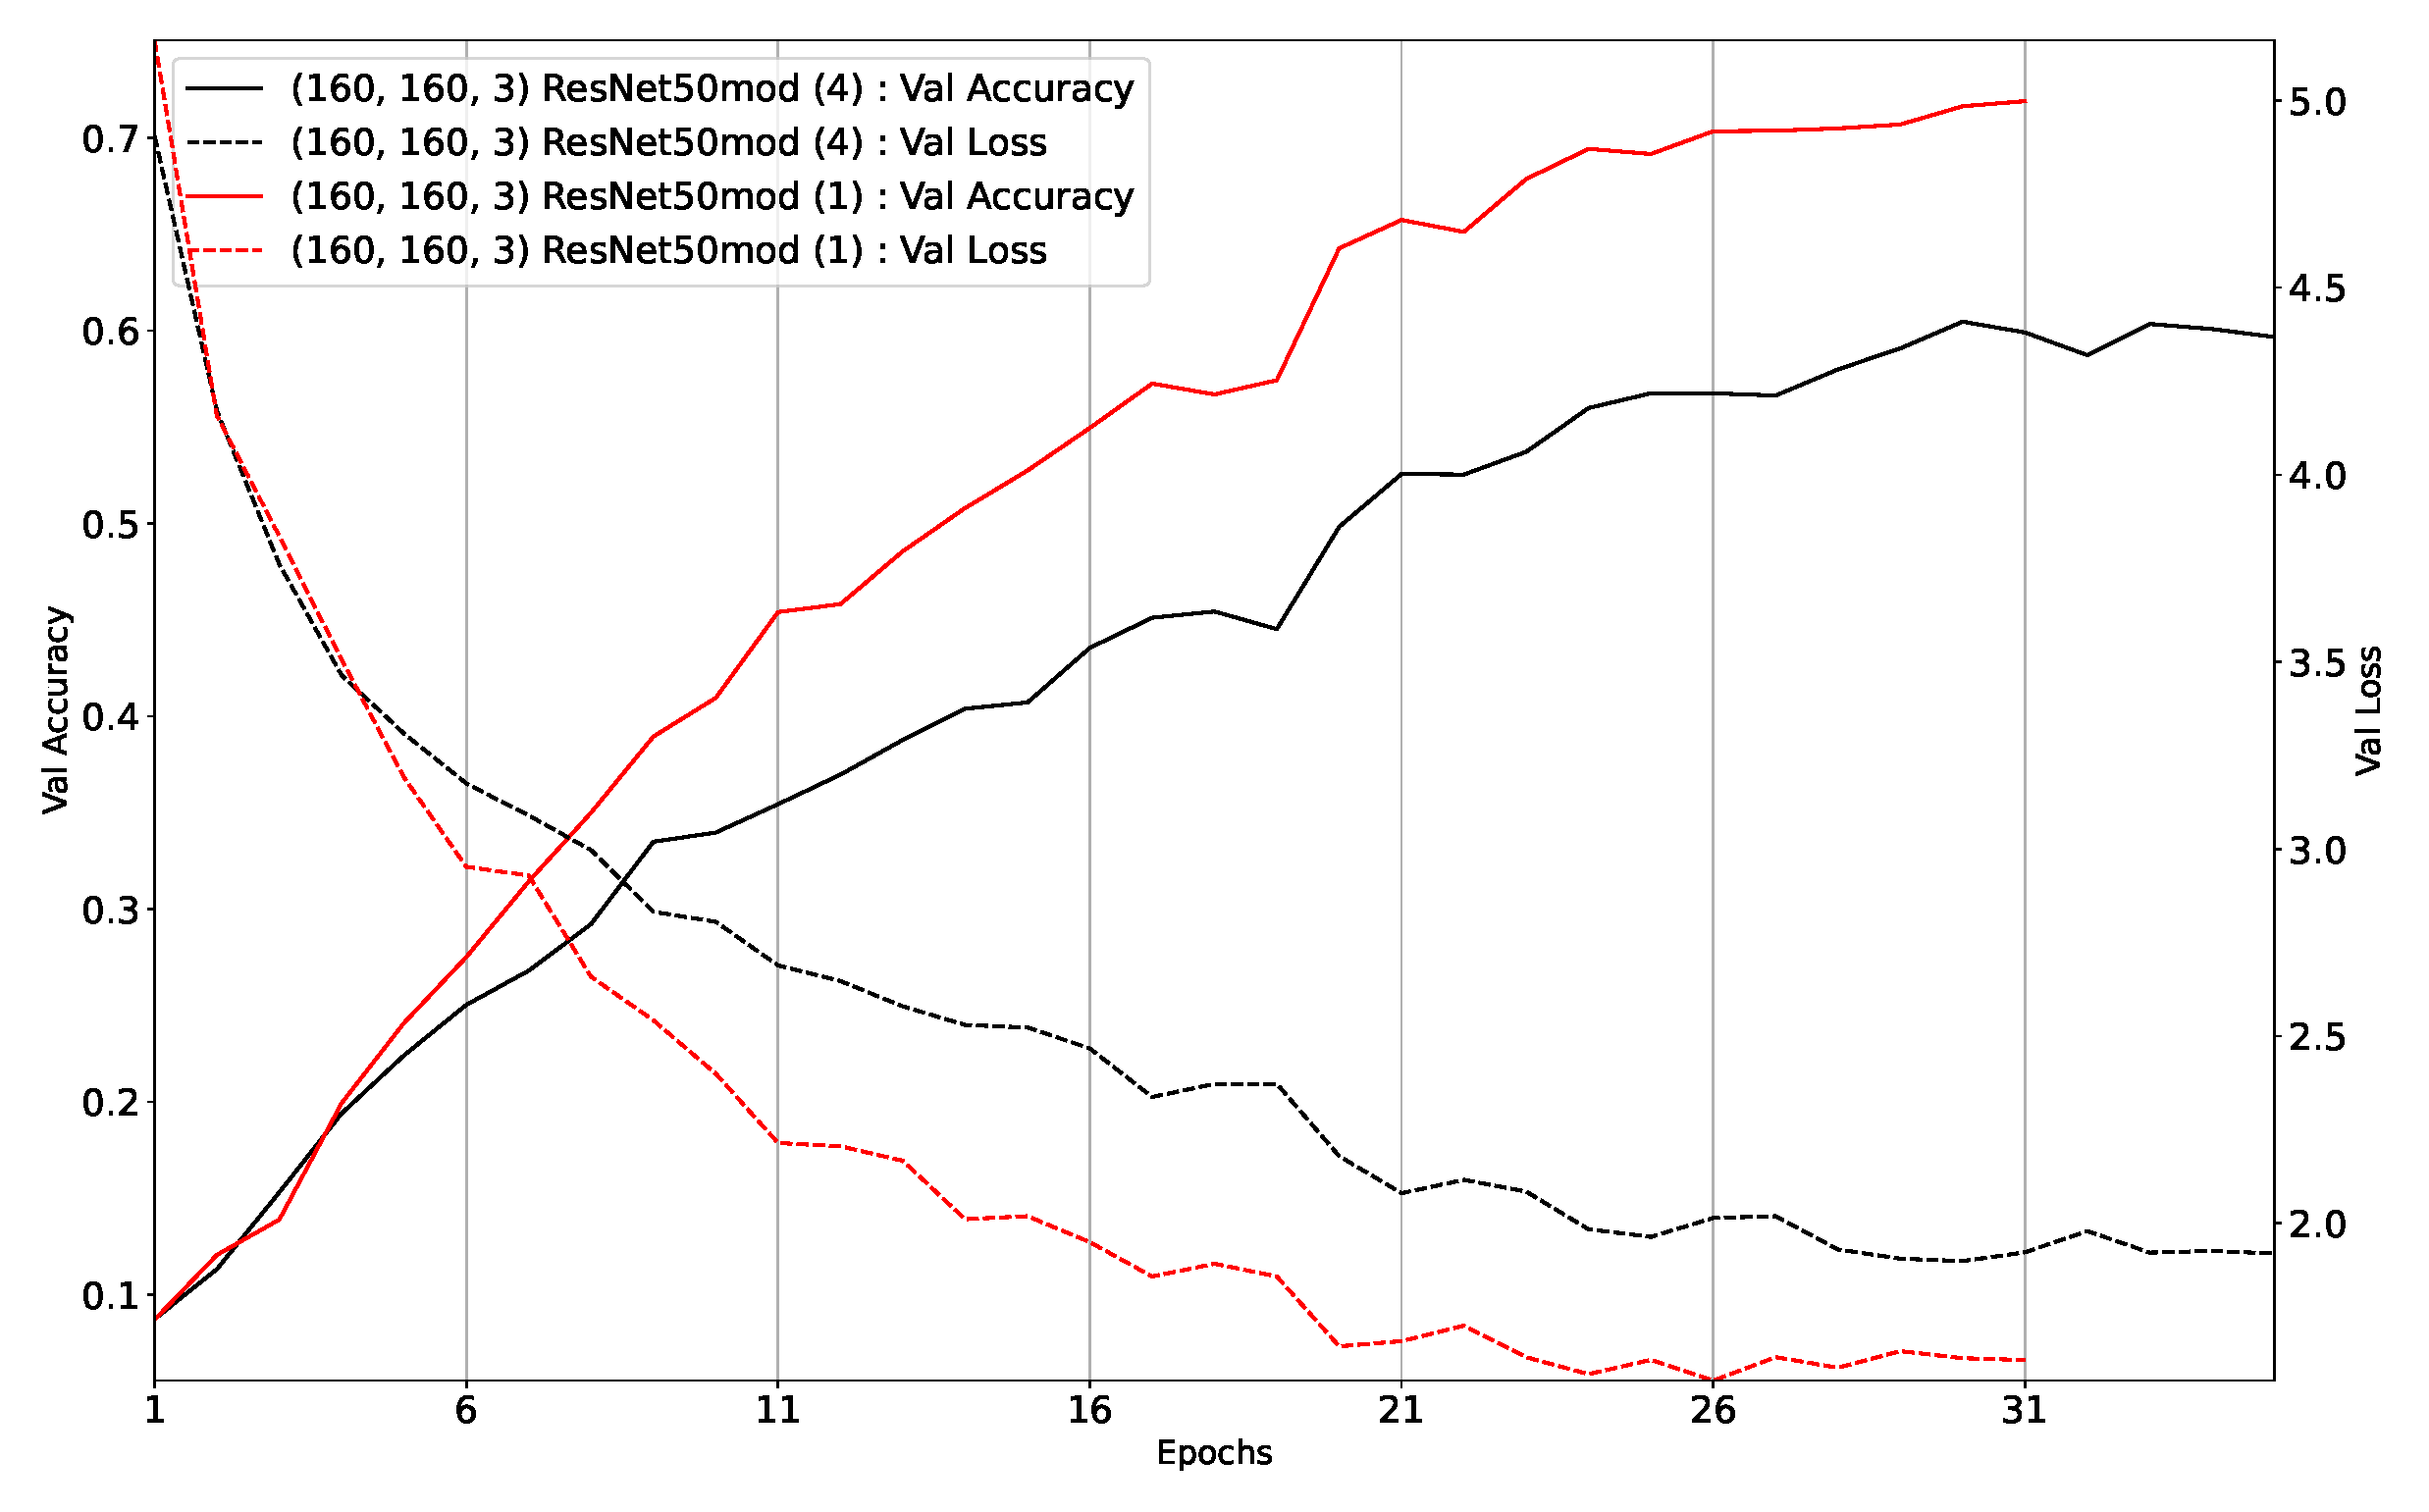
\includegraphics[width=\textwidth]{History_Compare_20unfrozen_0unfrozen_Validation.pdf}
\caption{Validation}
\label{image_unfrozen0_validation}
\end{subfigure}
\caption{Επίδραση ξεπαγώματος επιπέδων}
\label{Unfreeze_Layers_fig}
\end{figure}

\subsection{Επιλογή αρχιτεκτονικής}
\label{Architecture Selection}
Στις προηγούμενες παραγράφους παρουσιάστηκε η επίδραση που είχε στην εκπαίδευση μιας συγκεκριμένης αρχιτεκτονικής ένα πλήθος παραμέτρων όπως το μέγεθος των εικόνων, η χρήση image generator, καθώς και οι αποφάσεις που λήφθηκαν βασιζόμενοι σε αυτές τις δοκιμές. Η υπόθεση που έγινε ήταν ότι η συμπεριφορά που επιδείχθηκε στο τροποποιημένο μοντέλο ResNet50 θα ήταν ίδια και στα υπόλοιπα μοντέλα.

Έχοντας καταλήξει λοιπόν στο ποιο είναι το καταλληλότερο ResNet50mod παρουσιάζουμε στο σχήμα \ref{Training_History_Train} την εξέλιξη των τιμών ακρίβειας και της συνάρτησης κόστους για πέντε μοντέλα. Όπως γίνεται αντιληπτό το μοντέλο με την μεγαλύτερη ακρίβεια είναι το ResNet50mod για εικόνες (256, 256, 3) το οποίο και θα χρησιμοποιήσουμε στο επόμενο βήμα της εργασίας της μεταφοράς μάθησης. 


%\begin{figure}[H]
%\centering
%\begin{subfigure}[t]{1.0\textwidth}%
%\includegraphics[width=\textwidth]{History_Training.pdf}
%\end{subfigure}
%\caption{Ιστορία Εκπαίδευσης}
%\label{Training_History_Train}
%\end{figure}

\begin{figure}[H]
\centering
\begin{subfigure}[t]{1.0\textwidth}
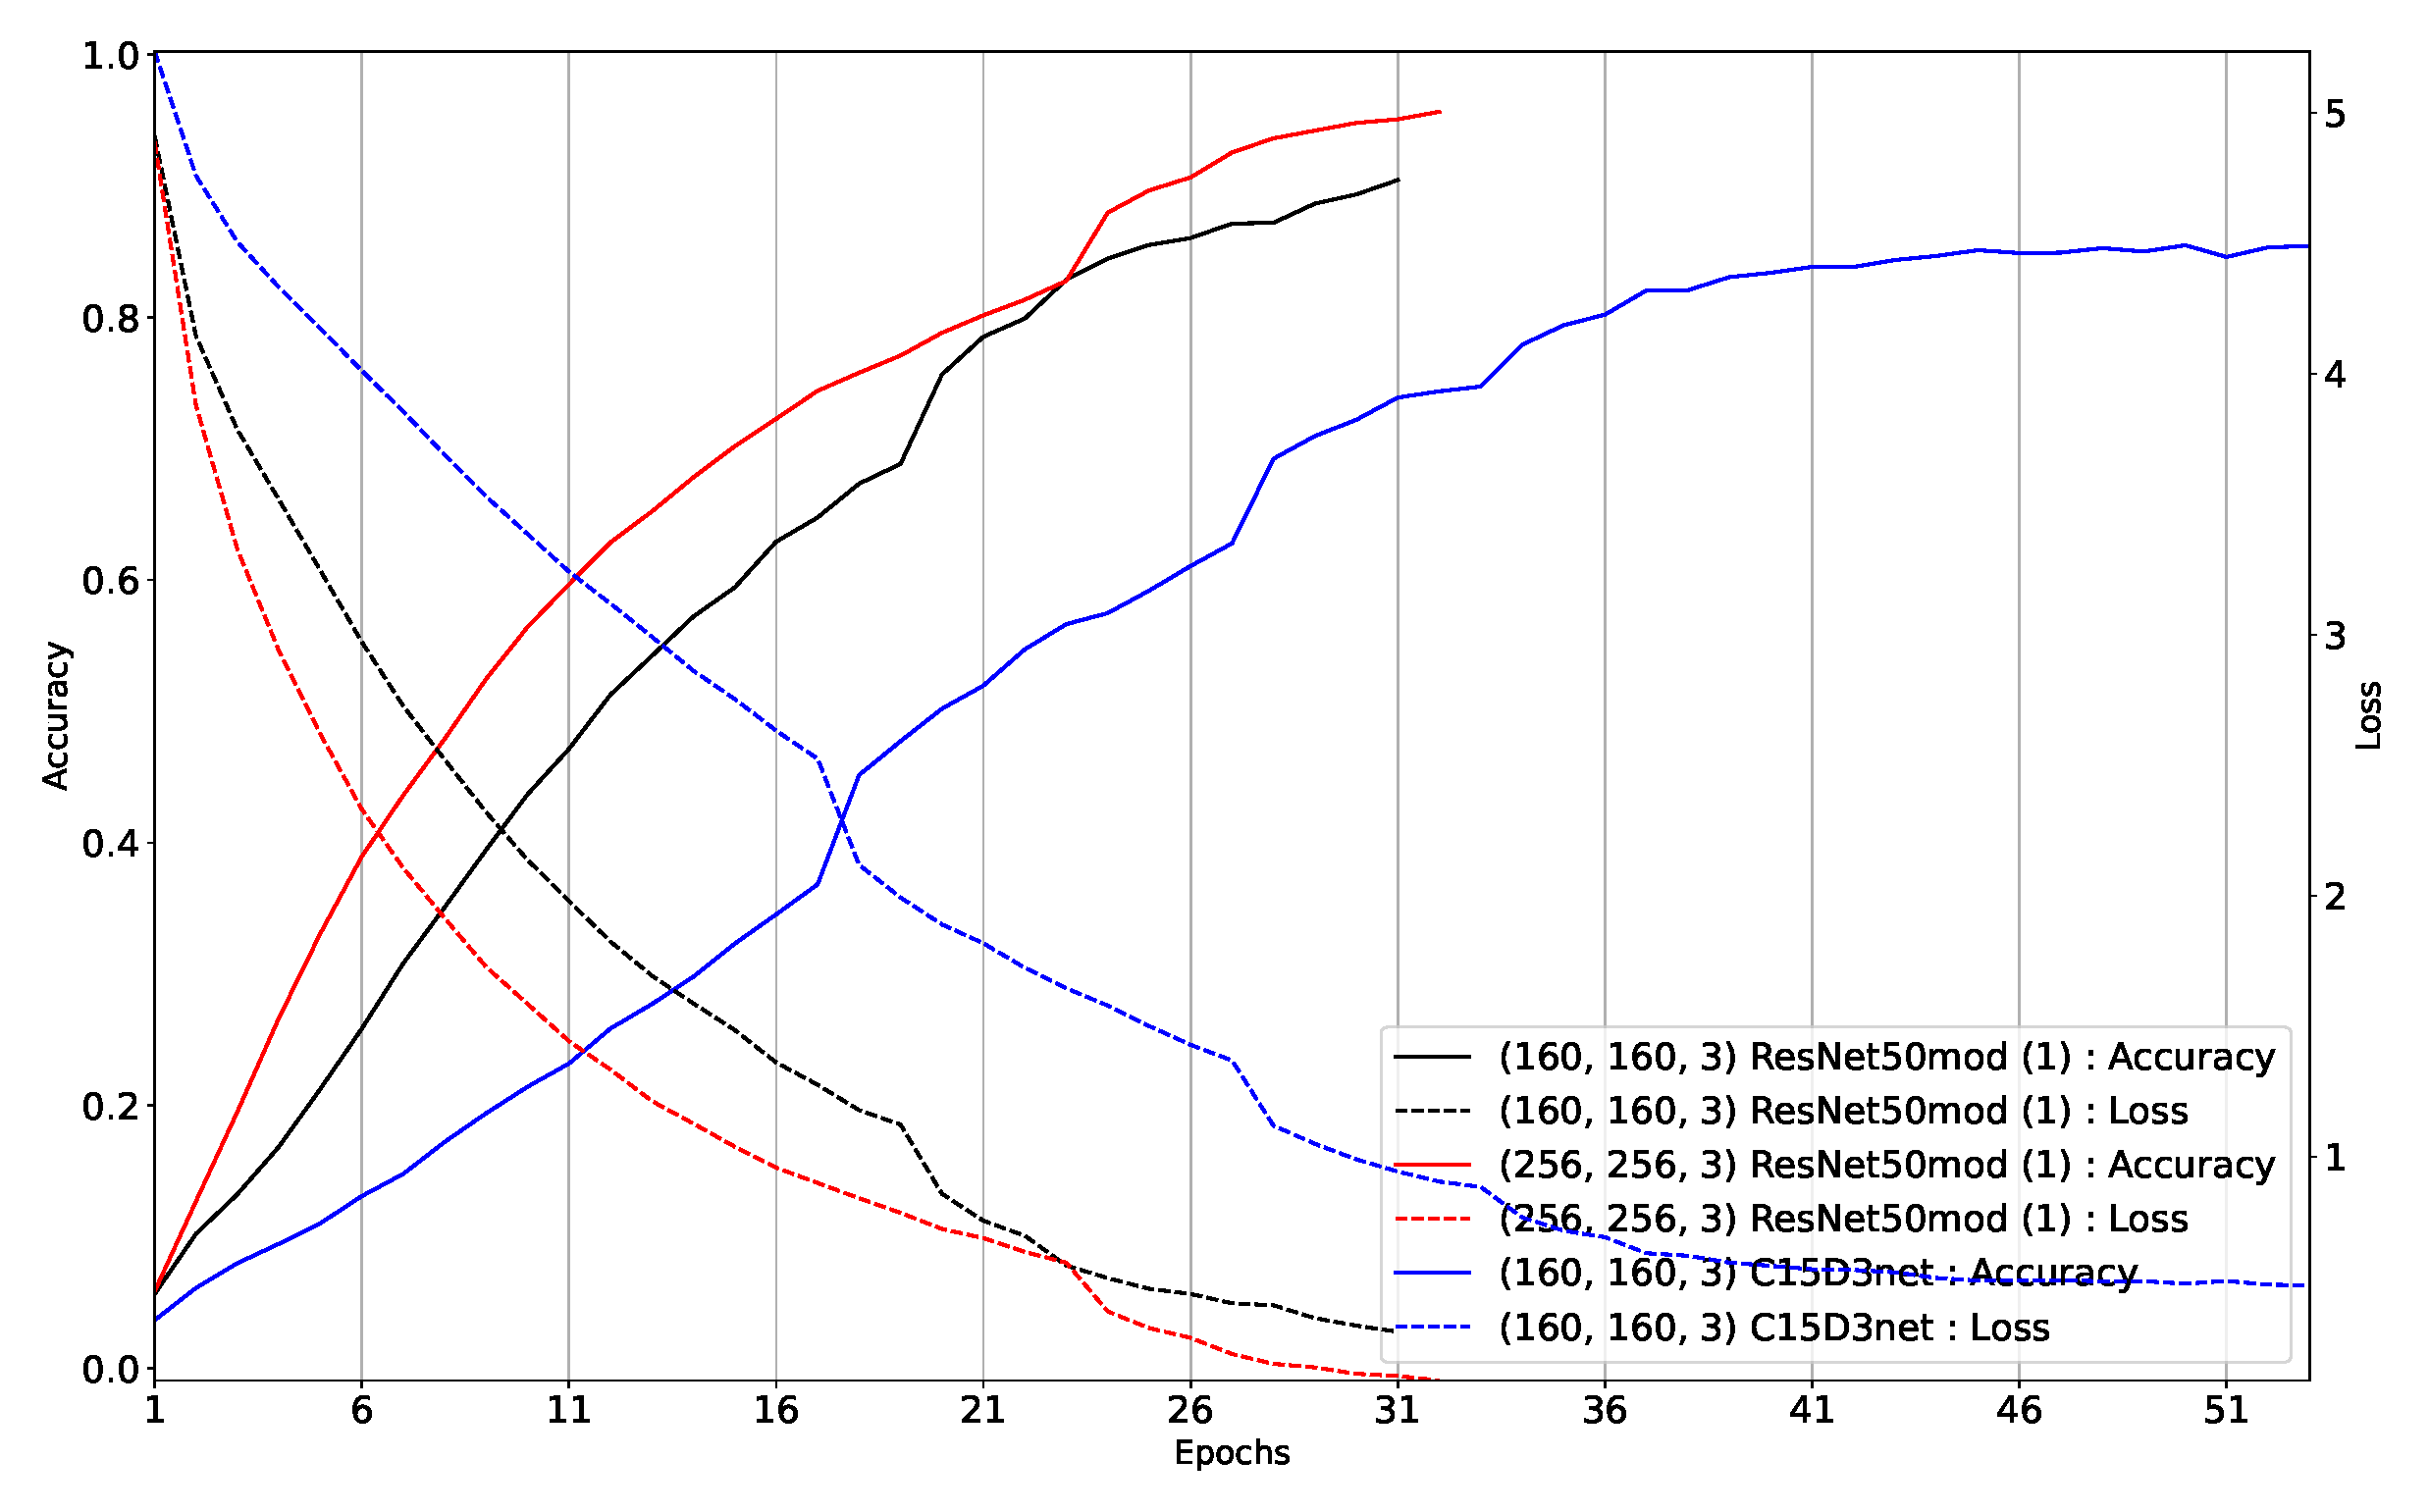
\includegraphics[width=\textwidth]{History_Compare_Models_160_Training.pdf}
\caption{Training}
\label{image_unfrozen20_training}
\end{subfigure}
\begin{subfigure}[t]{1.0\textwidth}
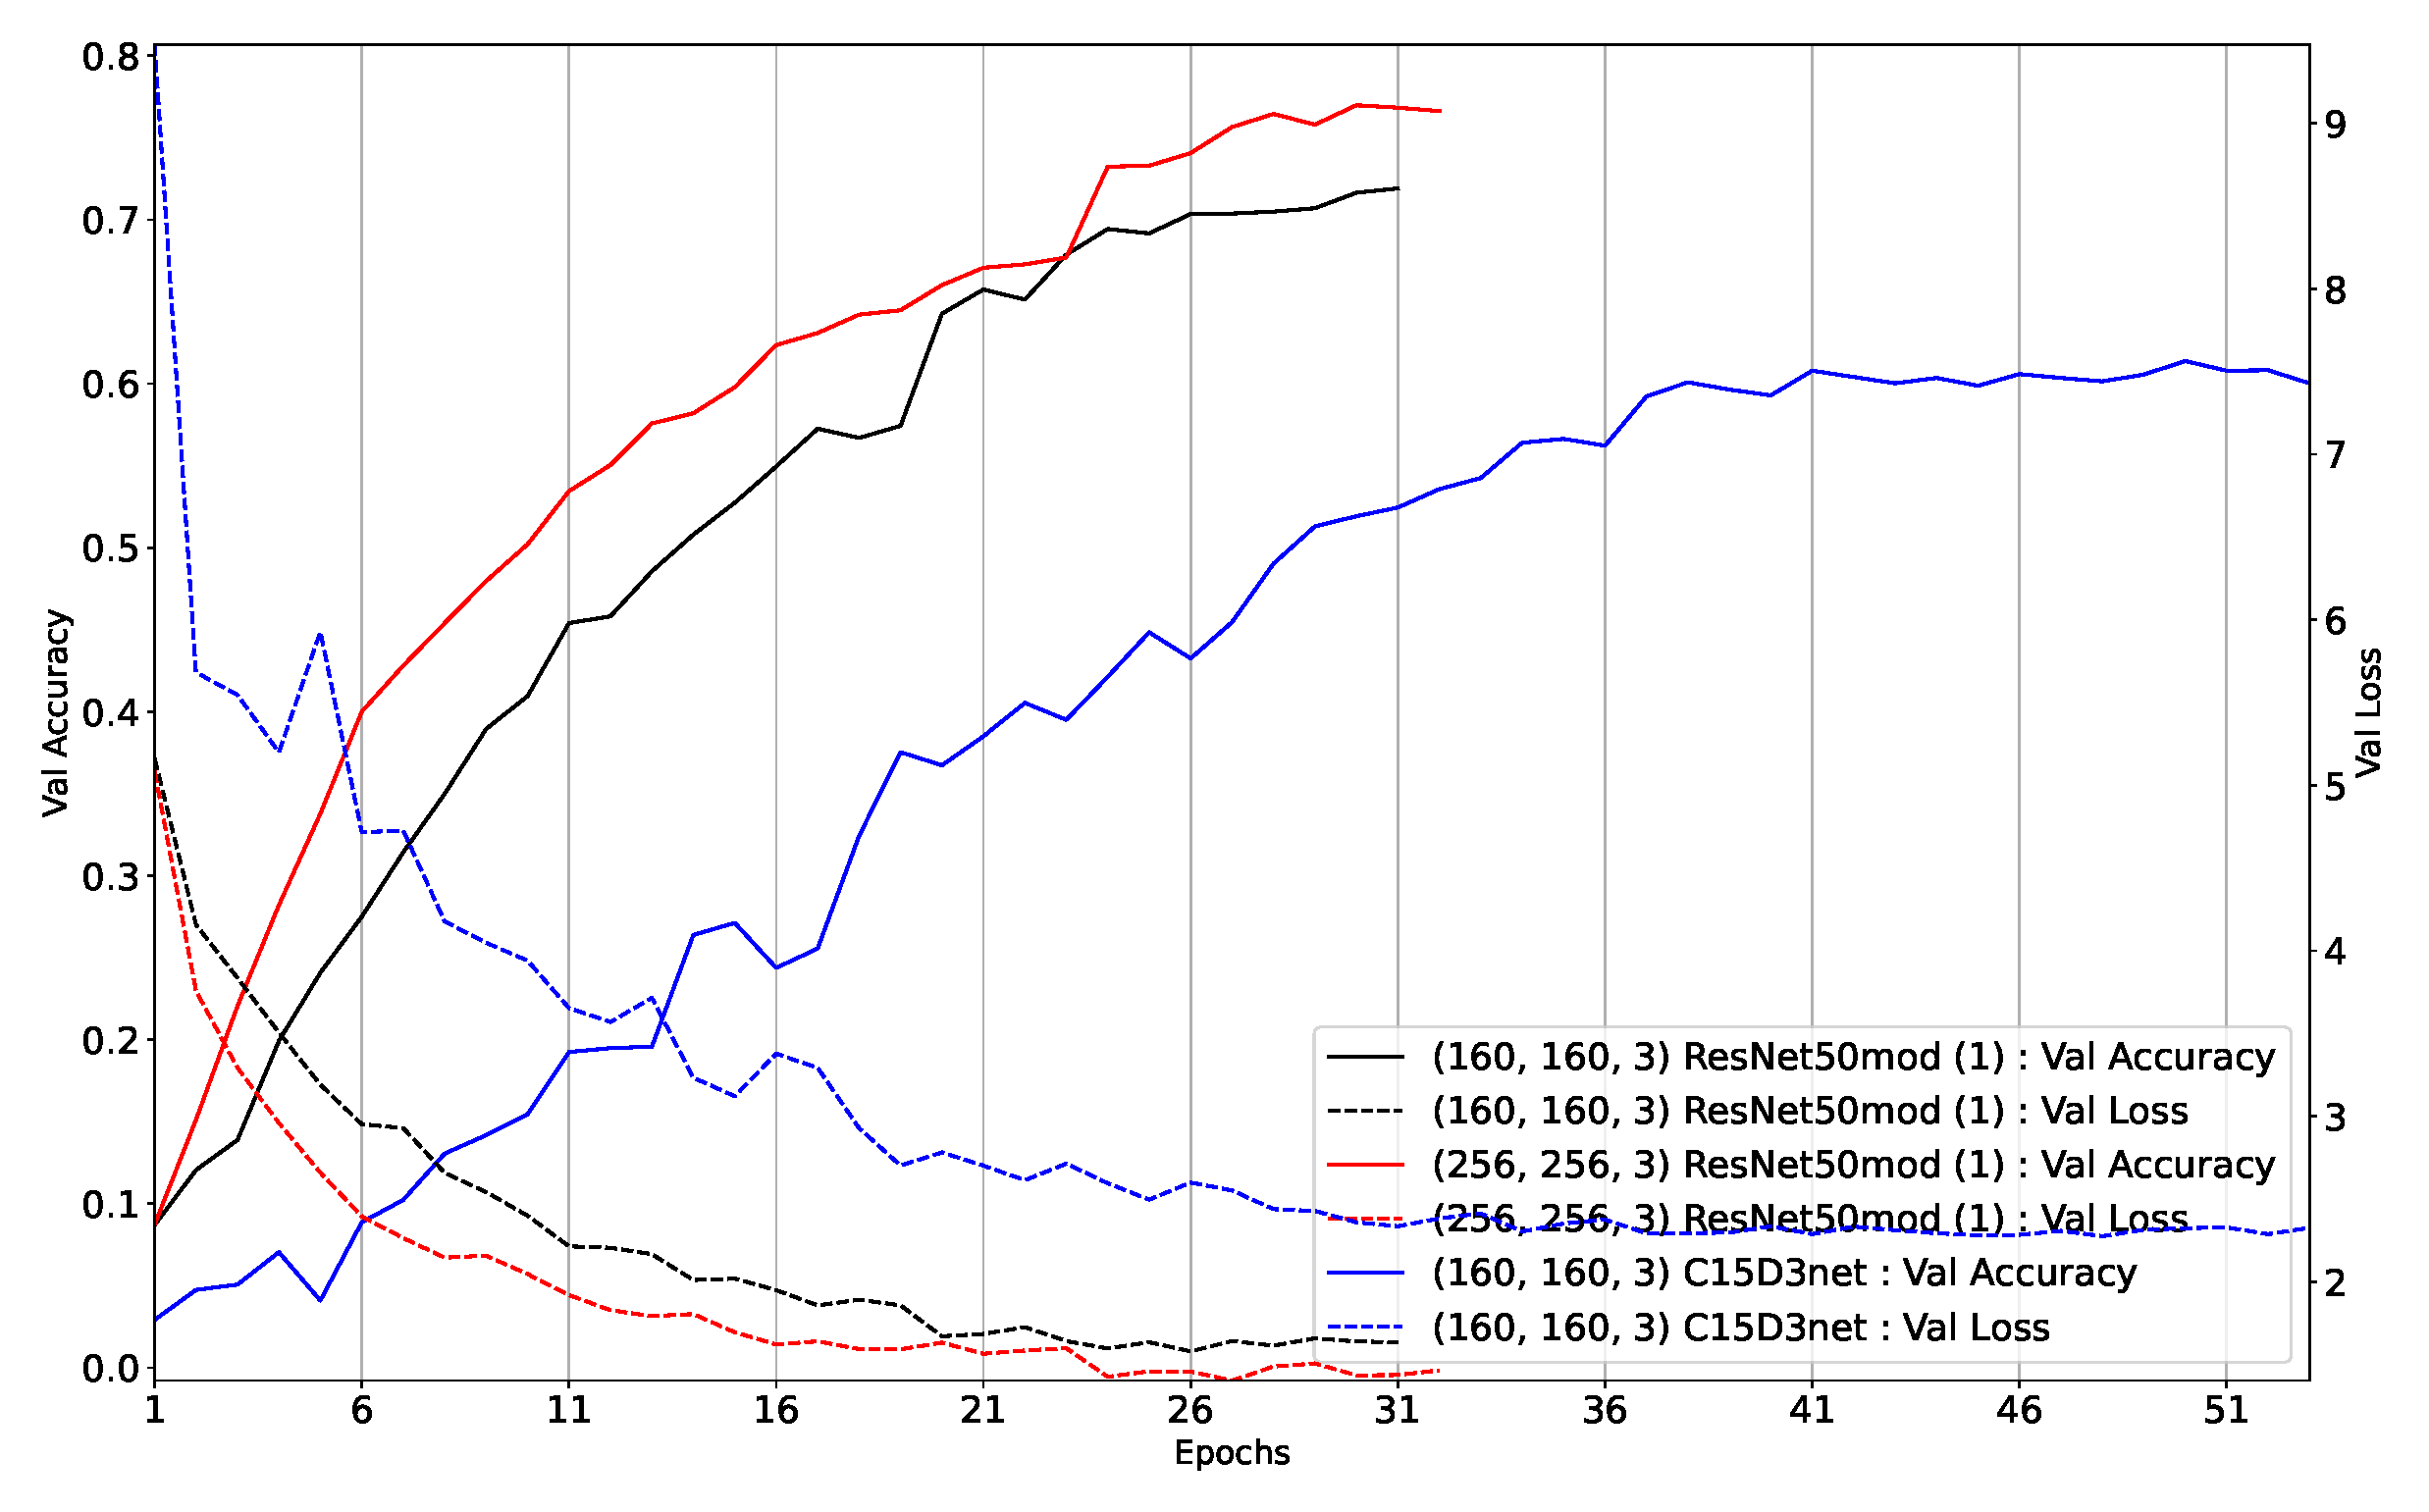
\includegraphics[width=\textwidth]{History_Compare_Models_160_Validation.pdf}
\caption{Validation}
\label{image_unfrozen0_validation}
\end{subfigure}
\caption{Ιστορία Εκπαίδευσης}
\label{Training_History_Train}
\end{figure}
\chapter{Μεταφορά μάθησης}
\thispagestyle{empty} % We remove page numbering
\vspace{-2em}
\section{Αρχιτεκτονική}
\label{ArchitectureUsed_transfer}

Όπως έχει ήδη αναφερθεί η εκπαίδευση του μοντέλου για την πρόβλεψη των εικόνων τροφής του συνόλου δεδομένων FOOD101 έγινε με τη χρήση της τεχνικής της μεταφοράς μάθησης. Για τον λόγο αυτό χρησιμοποιήθηκε το εκπαιδευμένο μοντέλο ResNet50mod για εικόνες εισόδου μεγέθους (256, 256, 3) και πάνω σε αυτό έγιναν οι αλλαγές που απαιτούνταν ώστε να προχωρήσει η εκπαίδευσή του.

Η μορφή της αρχιτεκτονικής αυτού του μοντέλου φαίνεται στο σχήμα \ref{transfer_learning_fig}, το οποίο μοιάζει πολύ με αυτό του σχήματος \ref{Pretrained_Architectures_fig} με ουσιαστικές όμως διαφορές που οπτικοποιούνται από τα διαφορετικά χρώματα των πλαισίων του σχήματος.  

Πιο αναλυτικά, με μαύρο χρώμα παριστάνονται τα τμήματα της αρχιτεκτονικής του δικτύου που μένουν ακριβώς ίδια όπως αυτά εκπαιδεύτηκαν κατά την ανάπτυξη του μοντέλου ResNet50mod. Με κόκκινο χρώμα φαίνονται τα τμήματα τα οποία αλλάζουν προαιρετικά και για τα οποία όπως φαίνεται στο σχήμα \ref{Training_History_Transfer} εκτελέστηκαν δοκιμές. Πρόκειται για το επιπλέον τμήμα συνελικτικών επιπέδων που είχε προστεθεί επί του προ-εκπαιδευμένου ResNet50. Τέλος, με μπλε χρώμα φαίνονται τα επίπεδα τα οποία είναι καινούρια και τα οποία πρακτικά αντικαθιστούν τα εξωτερικά πλήρως διασυνδεδεμένα επίπεδα της ResNet50mod.  

Με βάση λοιπόν αυτήν την αρχιτεκτονική εκτελέστηκαν τρεις διαφορετικές αξιολογήσεις οι οποίες συνοψίζονται παρακάτω, ενώ σχηματοποιούνται στο σχήμα \ref{Training_History_Transfer}.

\begin{enumerate}
\item ResNet50mod\_transfer (1) : 0 ξεπαγωμένα layers σε σχέση με την αρχιτεκτονική ResNet50mod
\item ResNet50mod\_transfer (2) : Ξεπάγωμα των τριών εξωτερικών συνελικτικών layers σε σχέση με την αρχιτεκτονική ResNet50mod
\item ResNet50mod\_transfer (3) : Ξεπάγωμα και των έξι εξωτερικών συνελικτικών layers σε σχέση με την αρχιτεκτονική ResNet50mod
\end{enumerate}

Τέλος δίνεται και ο πίνακας \ref{parameters_transfer_table}, όπου φαίνεται ο αριθμός των προς εκπαίδευση παραμέτρων για κάθε μια από τις τρεις περιπτώσεις, η οποία εξηγεί και τον λόγο που το ξεπάγωμα των έξι συνελικτικών επιπέδων οδηγεί σε μεγαλύτερη ακρίβεια πρόβλεψης.

\begin{table}[H]
\centering
\begin{tabular}{|c|c|}
\hline
Περίπτωση                 & Αριθμός παραμέτρων προς εκπαίδευση \\ \hline
ResNet50mod\_transfer (1) & 570,469                            \\ \hline
ResNet50mod\_transfer (2) & 9,225,829                          \\ \hline
ResNet50mod\_transfer (3) & 23,386,213                         \\ \hline
\end{tabular}
\caption{Αριθμός προς εκπαίδευση παραμέτρων}
\label{parameters_transfer_table}
\end{table}


\begin{figure}[H]
\centering
\begin{subfigure}[t]{1.0\textwidth}%
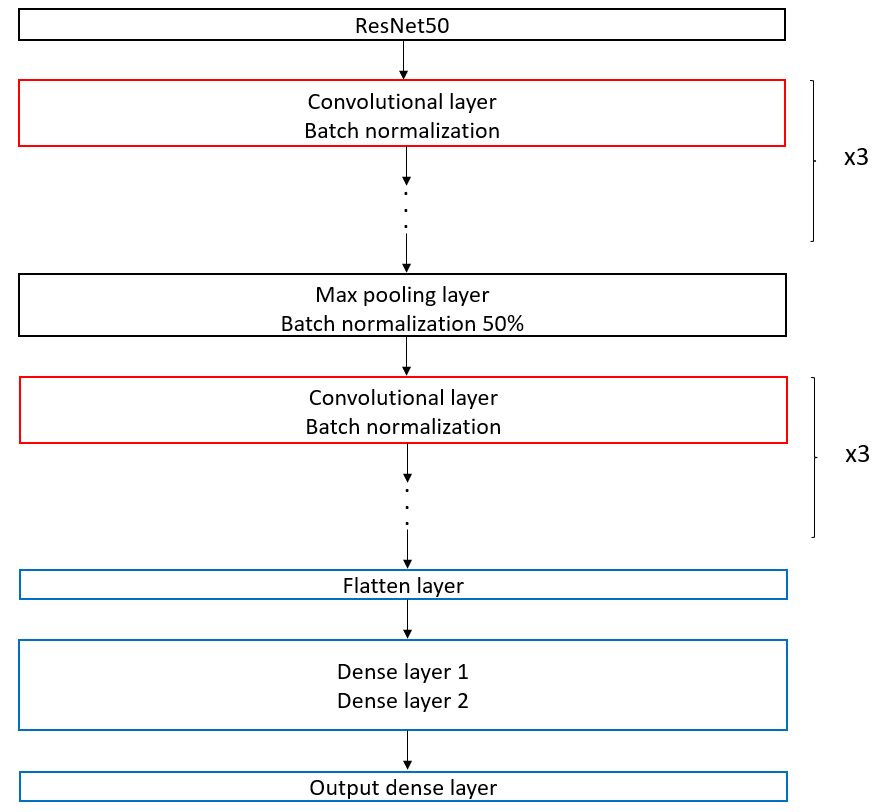
\includegraphics[width=\textwidth]{Transfer_Architecture.png}
\end{subfigure}
\caption{Αρχτιτεκτονική ResNet50mod (transfer learning)}
\label{transfer_learning_fig}
\end{figure}



\begin{figure}[H]
\centering
\begin{subfigure}[t]{1.0\textwidth}
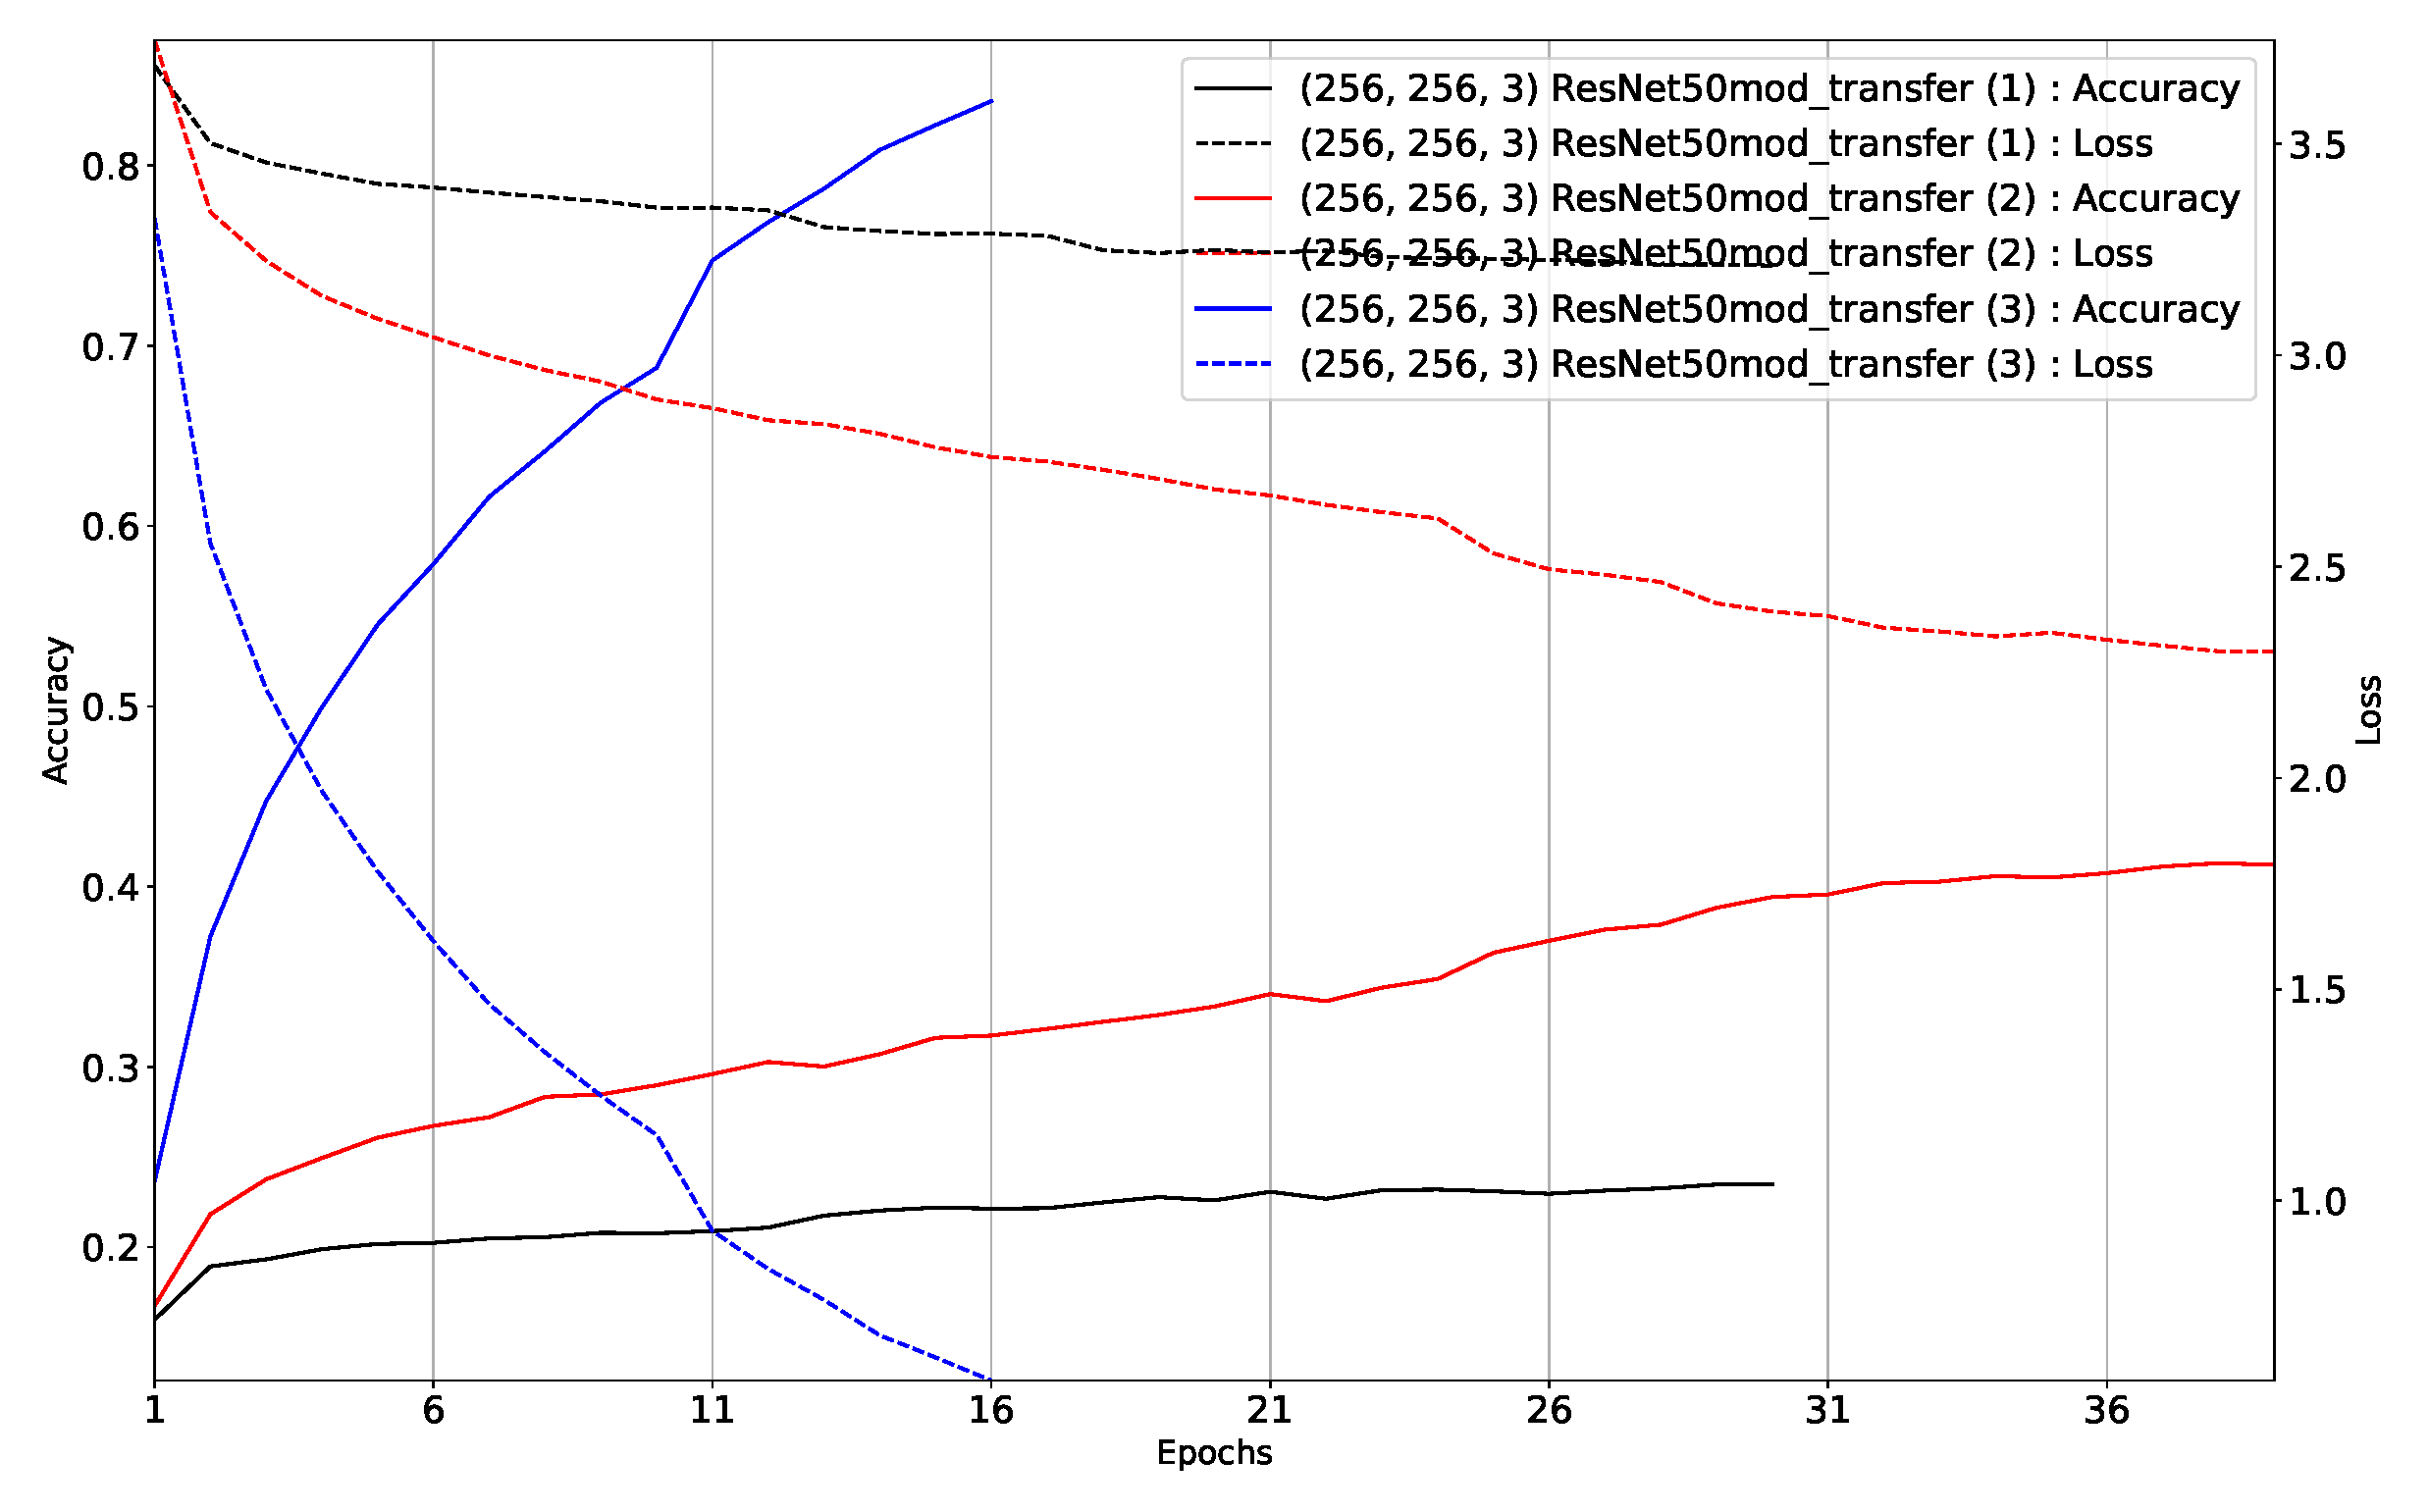
\includegraphics[width=\textwidth]{History_Transfer_Learning_Training.pdf}
\caption{Training}
\label{image_transfer_training}
\end{subfigure}
\begin{subfigure}[t]{1.0\textwidth}
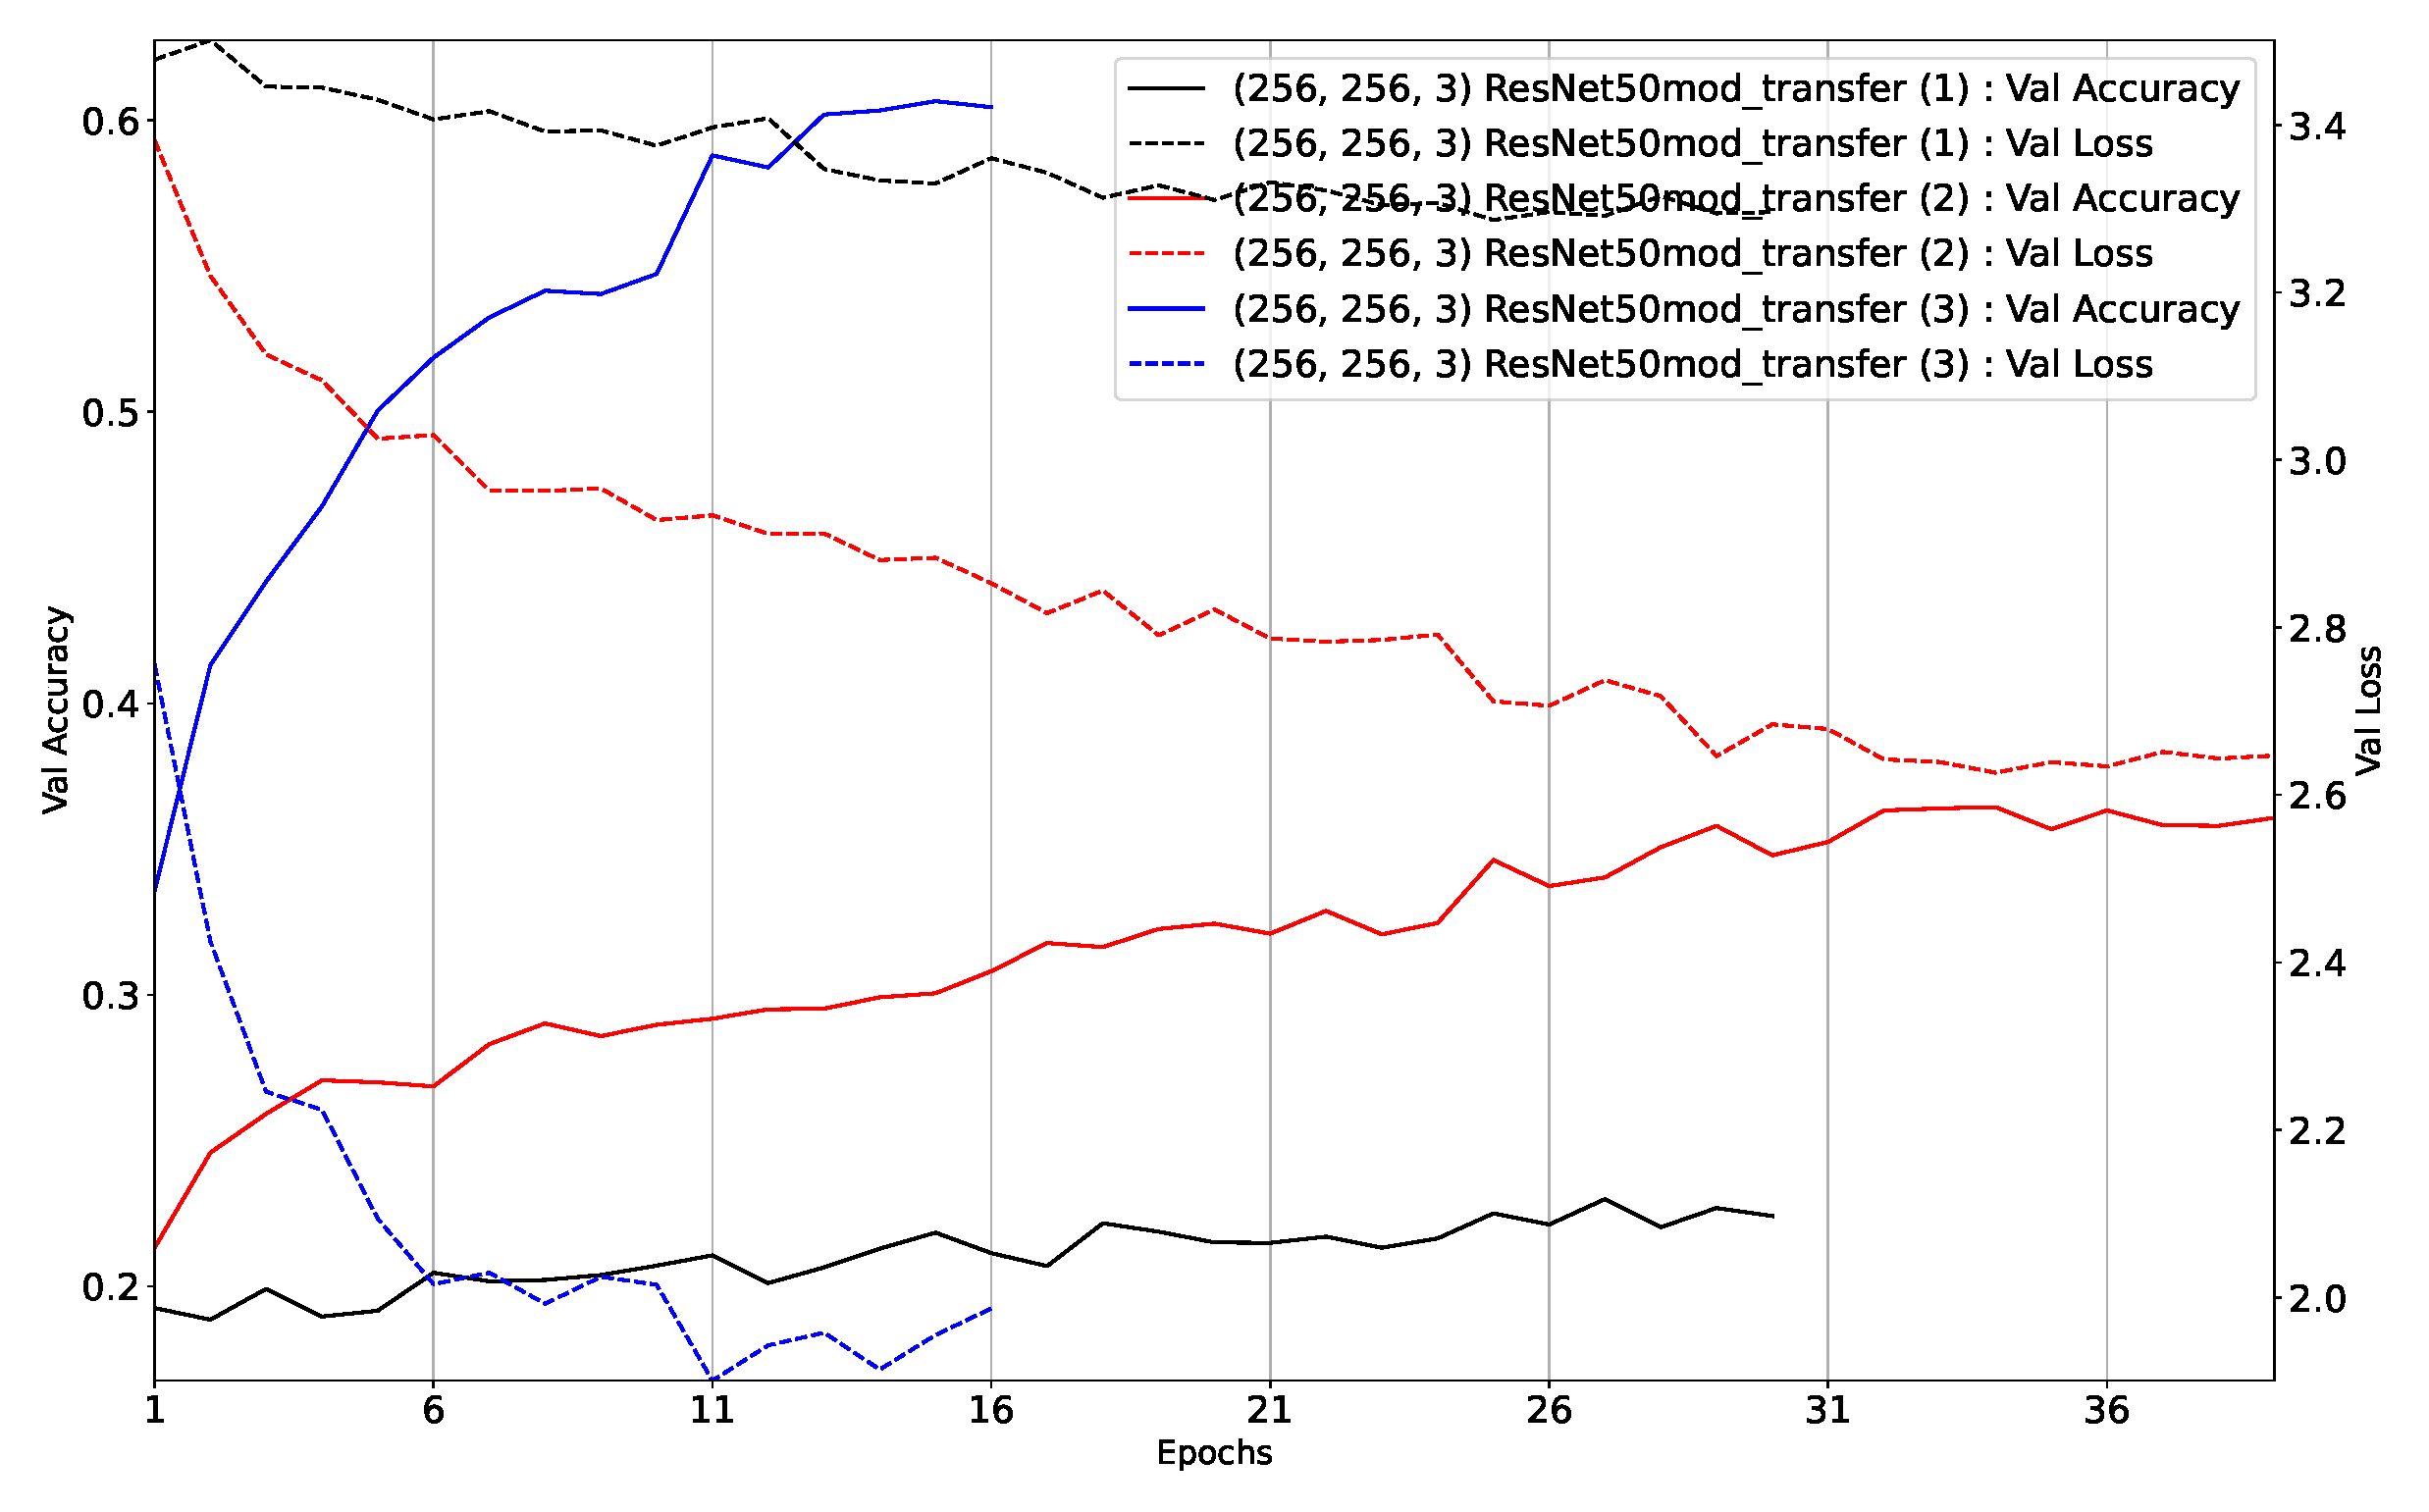
\includegraphics[width=\textwidth]{History_Transfer_Learning_Validation.pdf}
\caption{Validation}
\label{image_transfer_validation}
\end{subfigure}
\caption{Ιστορία εκπαίδευσης transfer learning}
\label{Training_History_Transfer}
\end{figure}




\chapter{Αποτελέσματα}
\thispagestyle{empty} % We remove page numbering
\vspace{-2em}
\section{Αποτελέσματα}
\label{Final_Results}

Στα τρία προηγούμενα κεφάλαια παρουσιάστηκε η διαδικασία εκπαίδευσης δύο νευρωνικών δικτύων ικανών να διακρίνουν και να ταξινομήσουν διαφορετικά είδη τροφών με τη χρήση εικόνων. Όπως αναφέρθηκε τα μοντέλα που επιλέξαμε ήταν το ResNet50mod (1) και το ResNet50mod\_transfer (3). 

Στον παρακάτω πίνακα \ref{final_results_table}
φαίνονται τα αποτελέσματα για την ακρίβεια, λεπτομέρεια (precision), ευαισθησία (recall) και την ακρίβεια top-5 για τα δύο μοντέλα. Επιπλέον στον ίδιο πίνακα αναγράφεται και η ακρίβεια αναφοράς (baseline accuracy) , η οποία ορίζεται ως η ακρίβεια που θα επιτύγχανε ένας αλγόριθμος που θα απέδιδε σε όλες τις παρατηρήσεις την πιο συχνά εμφανιζόμενη κατά την εκπαίδευση κλάση.  Σαν δεδομένα ελέγχου χρησιμοποιήθηκαν αυτά του test συνόλου δεδομένων που δεν είχαν χρησιμοποιηθεί μέχρι αυτό το τελικό στάδιο. Οι τρεις πρώτοι δείκτες υπολογίζονται από τις σχέσεις \ref{eval_relations}.  

Πρέπει να σημειωθεί ότι ενώ η ακρίβεια μπορεί να υπολογιστεί απευθείας διαιρώντας τις σωστές προβλέψεις με το σύνολο των προς πρόβλεψη σημείων, ο υπολογισμός για τους άλλους δύο δείκτες δεν είναι τόσο απλός. Αυτό γιατί πρέπει να υπολογιστεί η λεπτομέρεια (ή ισοδύναμα η ευαισθησία) για κάθε κλάση και στη συνέχεια παίρνοντας τον σταθμισμένο μέσο όρο να υπολογιστεί για το σύνολο του προβλήματος. 

Αναφορικά με τον ορισμό της ακρίβειας top-5, χρησιμοποιείται το ακόλουθο. Ο αλγόριθμος πρόβλεψης επιστρέφει τις πιθανότητες η κάθε εικόνα του test να ανήκει σε κάποια από τις 256 για το πρώτο ή 101 για το δεύτερο πρόβλημα κλάσεις. Έτσι αν η σωστή απάντηση βρίσκεται σε κάποια από τις πέντε επικρατέστερες κλάσεις τότε η απάντηση θεωρείται σωστή. 

Κλείνοντας στο σχήμα δίνεται ο πίνακας σύγχυσης (confusion matrix) \ref{confusion_matrix_fig_1} για το πρώτο πρόβλημα και αντίστοιχα στο σχήμα \ref{confusion_matrix_fig_2} για το δεύτερο πρόβλημα.

\begin{subequations} \label{eval_relations}
\begin{gather}
ACC=\dfrac{TP+TN}{P+N} \label{accuracy} \tag{4.1.1a}\\
PPV_{class}=\dfrac{TP}{TP+FP} \label{precision_PPV} \tag{4.1.1b}\\
SEN_{class}=\dfrac{TP}{TP+FN} \label{recall} \tag{4.1.1c}\\
\begin{cases}
\begin{aligned}
TP : True \, Positive, \, FP : False \, Positive \\
TN : True \, Negative, \, FN : False \, Negative 
\end{aligned} \tag{4.1.1e}
\end{cases}
\end{gather}
\end{subequations}


\begin{table}[H]
\centering
\begin{tabular}{|cc|cc|}
\hline
\multicolumn{2}{|c|}{UECFOOD256}         & \multicolumn{2}{c|}{FOOD101}            \\ \hline
\multicolumn{1}{|c|}{Baseline Accuracy}  & 0.02186 & \multicolumn{1}{c|}{Baseline Accuracy}       & 0.01386 \\ \hline
\multicolumn{1}{|c|}{Accuracy}       & 0.76751 & \multicolumn{1}{c|}{Accuracy}       & 0.63415 \\ \hline
\multicolumn{1}{|c|}{Top-5 Accuracy} & 0.90764 & \multicolumn{1}{c|}{Top-5 Accuracy} & 0.82607 \\ \hline
\multicolumn{1}{|c|}{Precision}      & 0.78941 & \multicolumn{1}{c|}{Precision}      & 0.64691 \\ \hline
\multicolumn{1}{|c|}{Recall}         & 0.76751 & \multicolumn{1}{c|}{Recall}         & 0.63534 \\ \hline
\end{tabular}
\caption{Τελικά αποτελέσματα}
\label{final_results_table}
\end{table}


\begin{figure}[H]
\centering
\begin{subfigure}[t]{1.0\textwidth}%
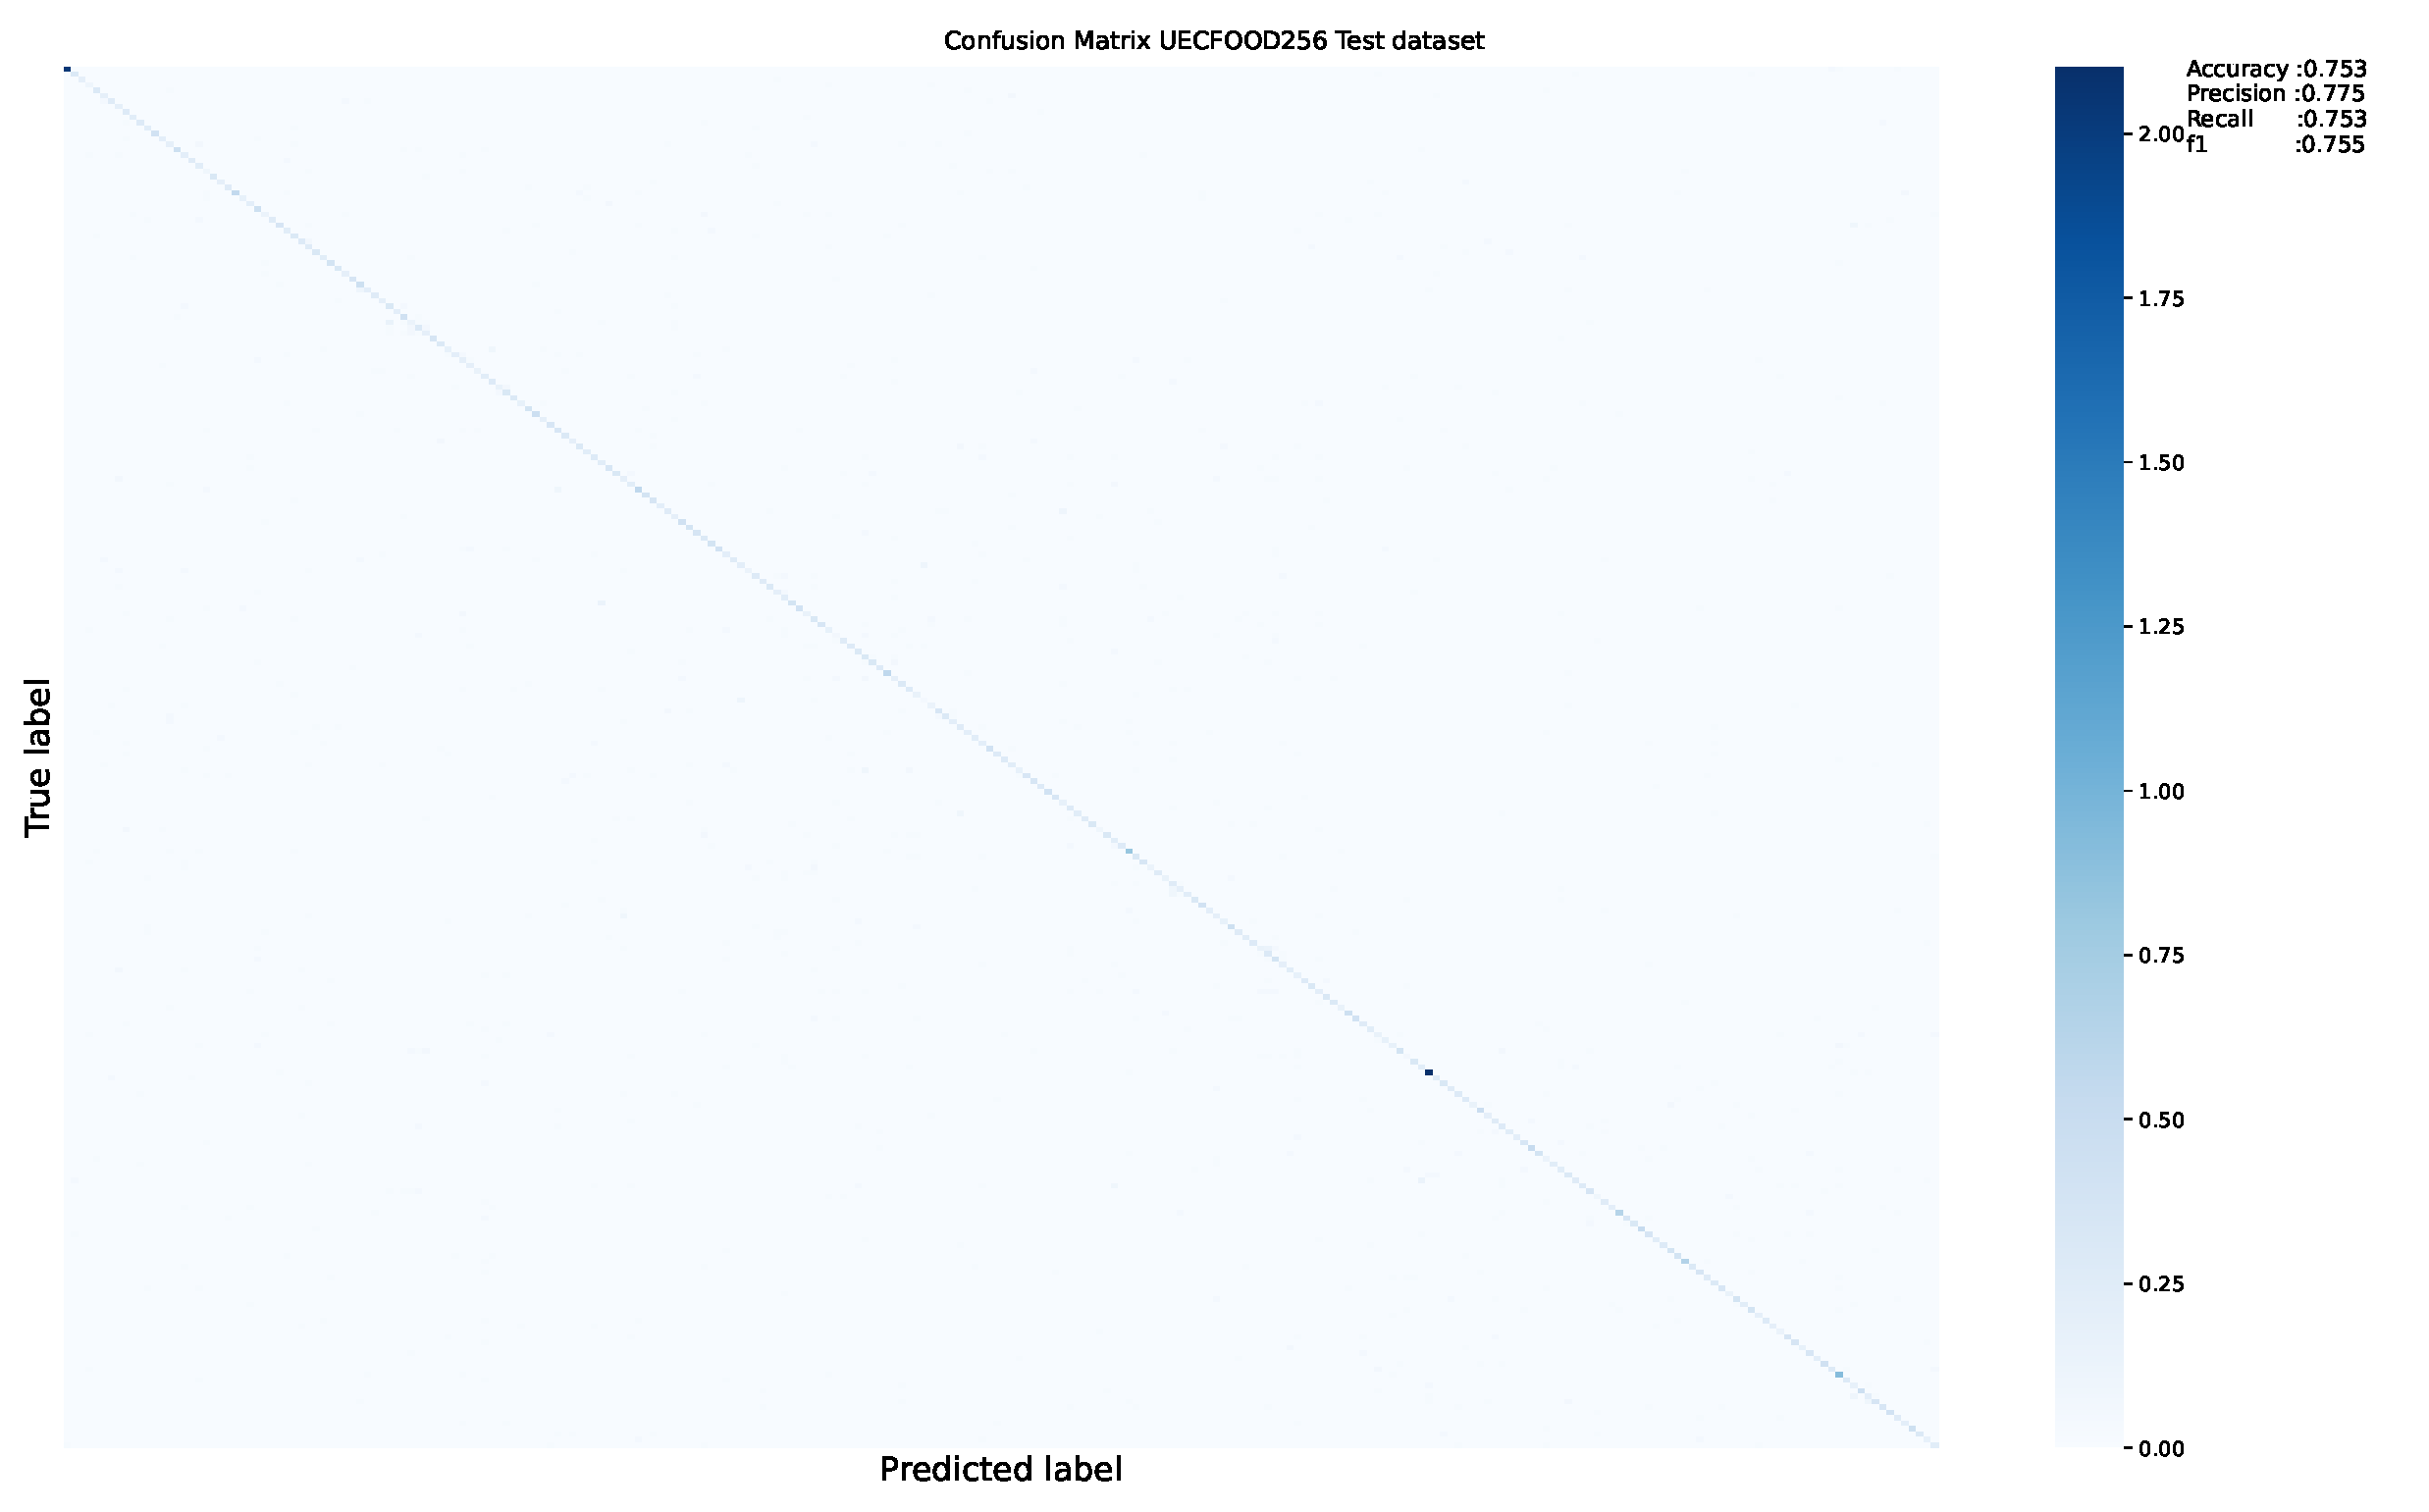
\includegraphics[width=\textwidth]{conf_matrix_dataset_1_(256, 256)_ResNet50mod_generator_2_regularizer_no_nlu1_20.pdf}
\end{subfigure}
\caption{Confusion matrix ResNet50mod}
\label{confusion_matrix_fig_1}
\end{figure}


\begin{figure}[H]
\centering
\begin{subfigure}[t]{1.0\textwidth}%
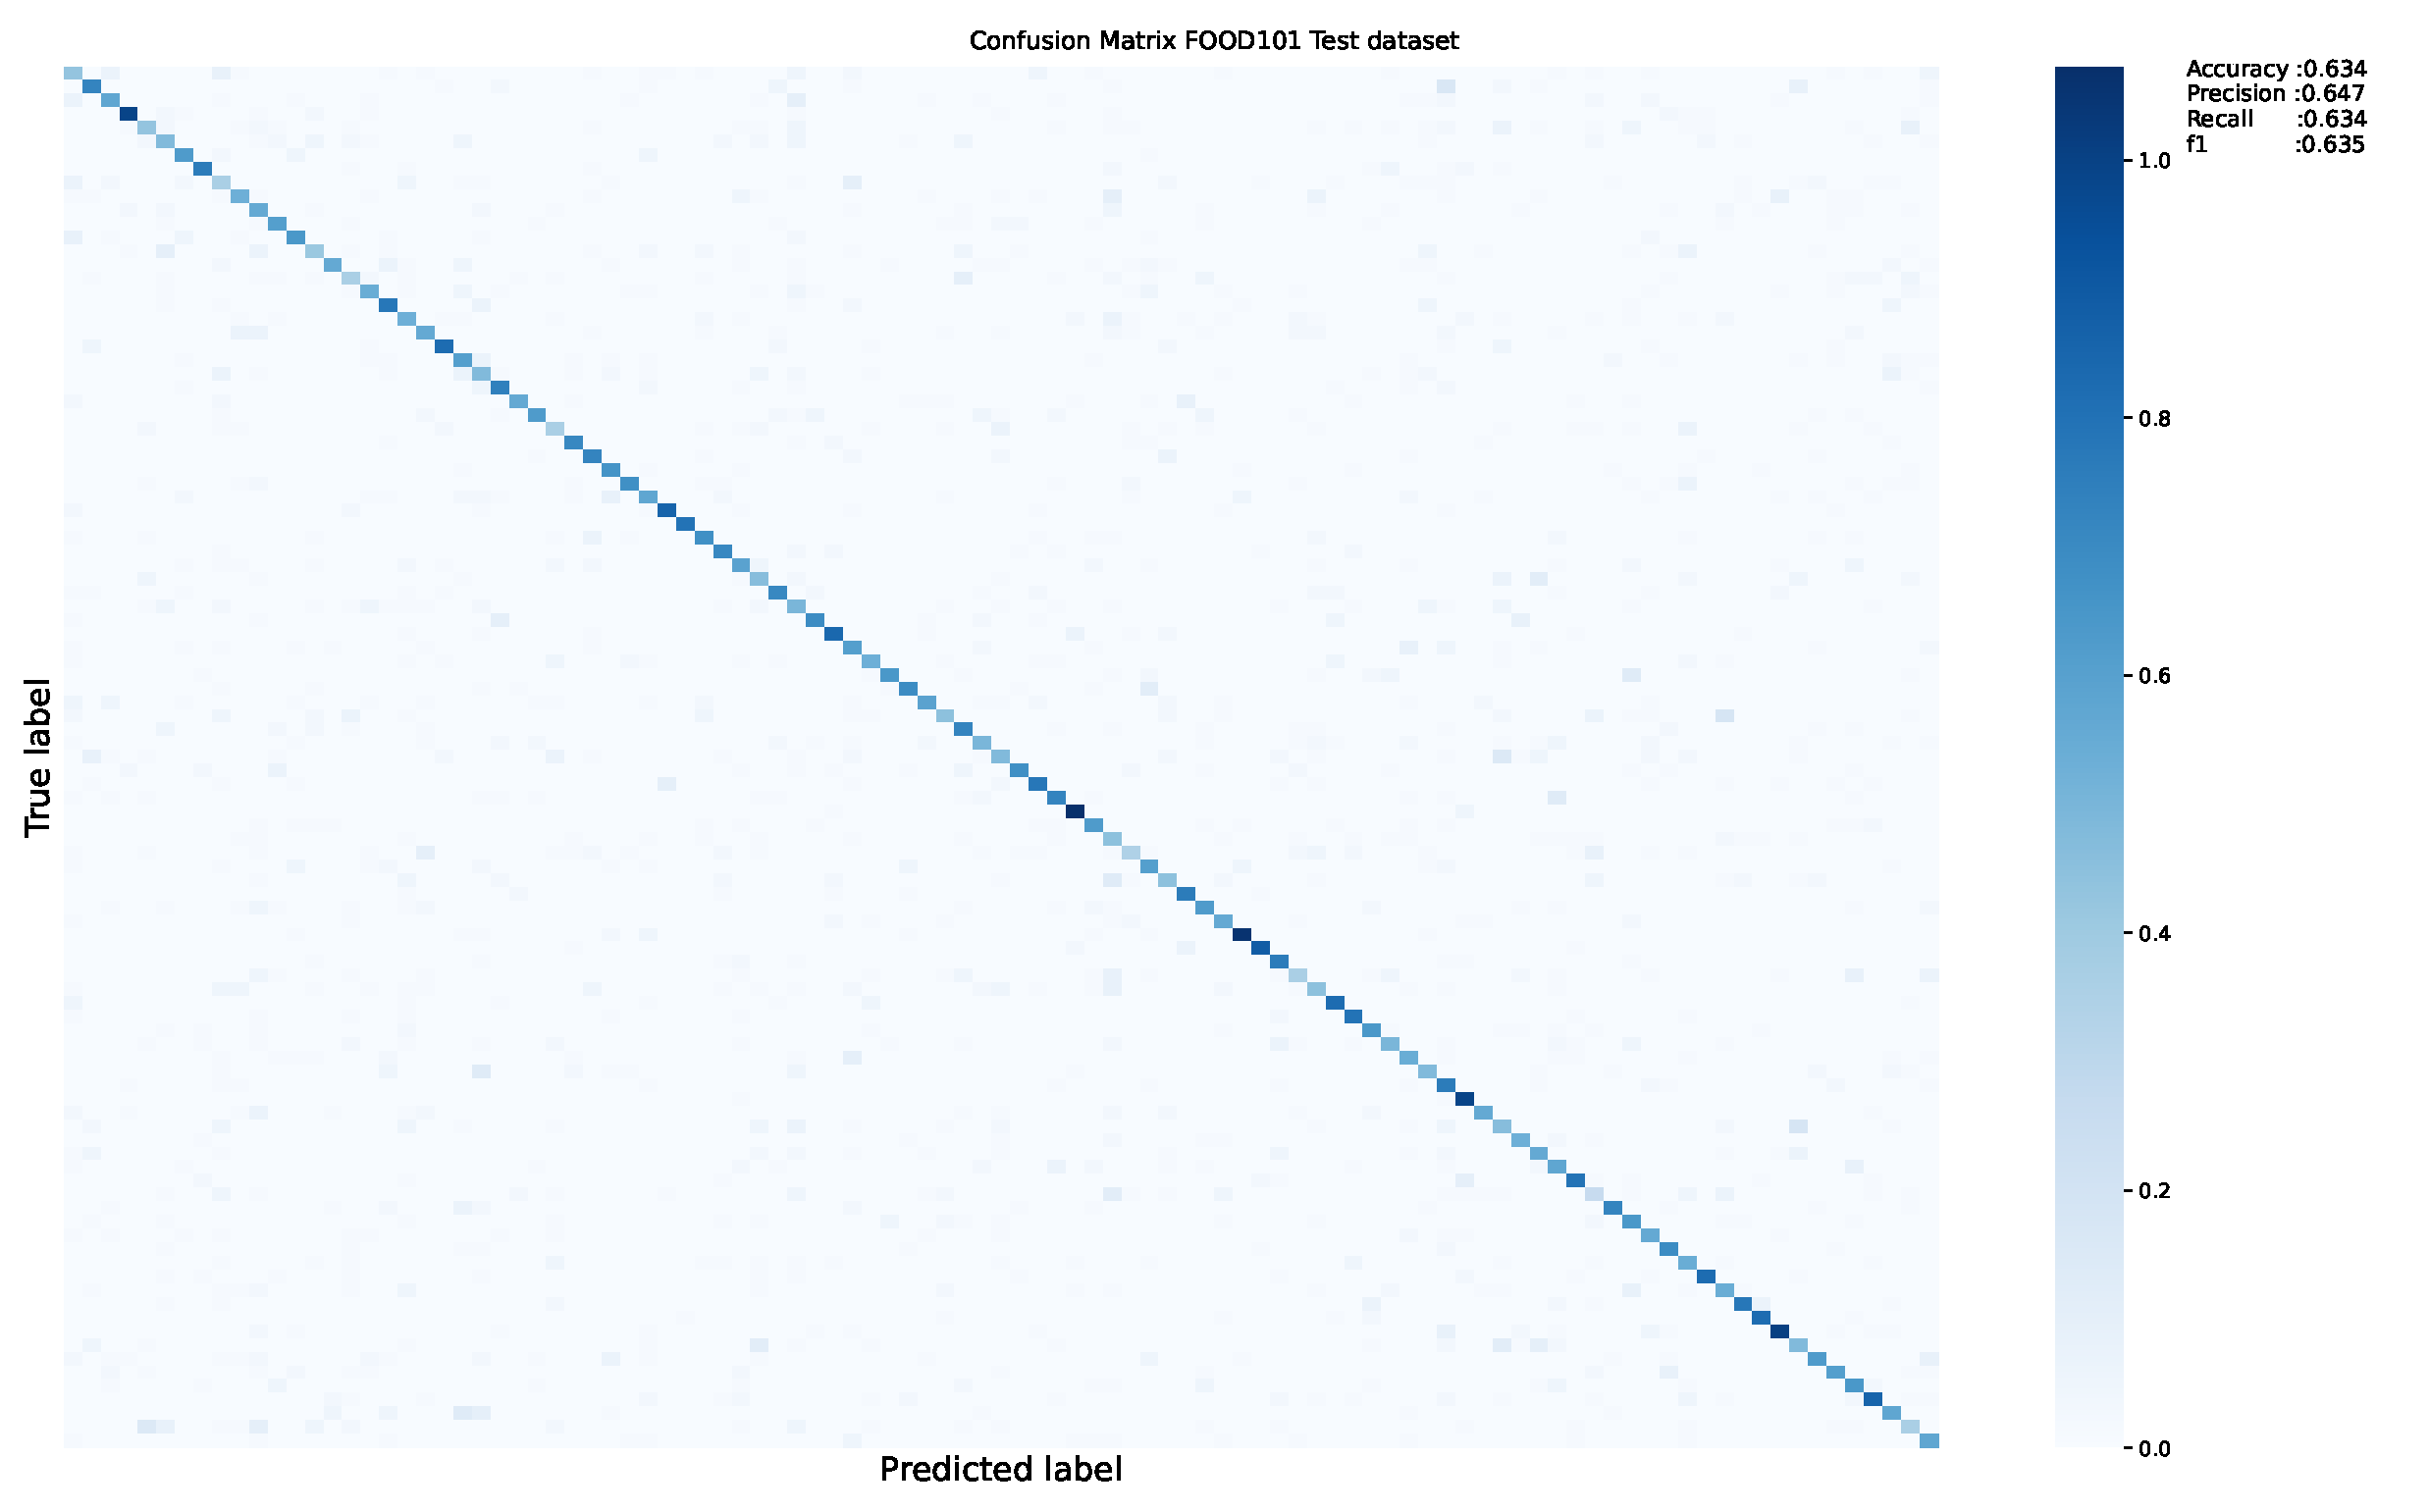
\includegraphics[width=\textwidth]{conf_matrix_dataset_2_(256, 256)_ResNet50mod_generator_2_regularizer_no_nlu1_20_nlu2_14.pdf}
\end{subfigure}
\caption{Confusion matrix ResNet50mod\_transfer}
\label{confusion_matrix_fig_2}
\end{figure}



\section{Συμπεράσματα}
\label{Conclusions}

Οι προκλήσεις που αντιμετωπίστηκαν κατά τη διάρκεια της εκπαίδευσης οφείλονταν σε μια σειρά παραμέτρων και περιγράφηκαν σε διάφορα σημεία της αναφοράς. Συνοπτικά μπορούν να κατηγοριοποιηθούν στις παρακάτω κατηγορίες.

\begin{enumerate}
\item Επάρκεια υπολογιστικών πόρων (μνήμης RAM) και χρόνου εκτέλεσης
\item Πλήθος υπερπαραμέτρων και εντοπισμός βέλτιστης λύσης 
\item Προλήματα overfitting και underfitting
\end{enumerate}


Αναλυτικότερα, η επάρκεια υπολογιστικών πόρων είναι σημαντική για όλα τα προβλήματα deep learning καθώς ο όγκος των δεδομένων είναι ιδιαίτερα μεγάλος με αποτέλεσμα ένας απλός οικιακός υπολογιστής να μην μπορεί να ανταπεξέλθει. Το πρόβλημα δεν αφορά μόνο την ταχύτητα επεξεργασίας των δεδομένων, αλλά επίσης και τις απαιτήσεις σε μνήμη RAM. Για τον λόγο αυτό, στην παρούσα εργασία ήταν αδύνατον να χρησιμοποιηθεί κάποιο υπάρχον διαδικτυακό μέσον που εκτελεί τον κώδικα παράλληλα, καθώς η RAM ξεπερνούσε τα 25-30 GB με αποτέλεσμα να μην μπορεί να εκτελεστεί. Έτσι καταφύγαμε στη λύση του οικιακού υπολογιστή με αποτέλεσμα να μην παραλληλοποιηθεί η διαδικασία μας.

Το πλήθος των υπερπαραμέτρων προς προσδιορισμό (tuning) είναι πολύ μεγάλο και όπως είδαμε λόγω και του αυξημένου χρόνου είναι αδύνατο να κάνουμε ακριβή προσδιορισμό του βέλτιστου συνδυασμού. Κατά συνέπεια, μελετήθηκαν κάποιες  ενδεικτικές περιπτώσεις, οπότε είναι πιθανό ότι μια πιο ενδελεχής δοκιμή υπερπαραμέτρων θα οδηγούσε σε ακόμη καλύτερα αποτελέσματα.

Τα προβλήματα overfitting και underfitting ήταν παρόντα σε διάφορες περιπτώσεις. Έτσι όταν δεν είχαμε πολλά layers προς εκπαίδευση δεν πετυχαίναμε επαρκή ακρίβεια, ενώ αντίθετα όσο αυξάναμε τα layers αύξανε η ακρίβεια αλλά υπήρχε overfitting. Για αυτό το λόγο, χρησιμοποιήσαμε dropout layers το οποίο φάνηκε να βοηθάει τα τελικά αποτελέσματα. Εκ νέου όμως το υπολογιστικό κόστος ήταν απαγορευτικό για μια βαθύτερη μελέτη.

%\backmatter
%------------The Bibliography I used-----------------------
\renewcommand{\thepage}{}
\bibliographystyle{plain}
\nocite{*}%With this command we put our references in Bibliography
\bibliography{Κεφάλαια/Βιβλιογραφία}
%---------------------------------------------------
\end{document}